\section{张量分解}\label{chapter:tensor-decomposition}
处理高阶张量的计算代价很高，因为元素个数随张量的阶呈指数增长。为应对这一问题，张量分解应运而生，成为有力而高效的工具。
与矩阵分解类似，张量分解把一个高阶张量拆成阶数更低、元素更少的若干小分量，从而使计算更易处理。但矩阵秩的概念可以以多种方式推广到张量，每种推广都对应一种不同的因子化/分解模型。
本章介绍最广为人知的几种张量分解模型。
\subsection{并行因子/CP 分解（CANDECOMP/PARAFAC~Decomposition）}\label{sec:cp-decomposition}
$N$ 阶张量 $\At\in\RR^{d_1\times\cdots\times d_N}$ 的 CP 分解~\citep{hitchcock1927expression}把 $\At$ 分解为有限个秩一张量之和。等价地，它是 $R$ 个秩一张量的线性组合，其中 $R$ 称为该分解的秩：
$$\At = \sum_{r=1}^R \ab^{(r)}_1\outprod\dots\outprod\ab^{(r)}_N ,$$
其中对每个 $n\in [N]$，都有 $\ab^{(1)}_n,\dots,\ab^{(R)}_n\in\RR^{d_n}$。

把所有向量 $\ab^{(r)}_n$ 排成因子矩阵，
\[\Ab_1 = {\begin{pmatrix}
\ab^{(1)}_1 & \dots & \ab^{(R)}_1 \\
\end{pmatrix}}{\in\RR^{d_1\times R}}, \dots ,\Ab_N = {\begin{pmatrix}
\ab^{(1)}_N & \dots & \ab^{(R)}_N \\
\end{pmatrix}}{\in\RR^{d_N\times R}}, \]
CP 分解可简洁地记作 $\At = \CP{\Ab_1,\cdots,\Ab_N}$。

在张量网络中，CP 分解 $\At = \CP{\Ab,\Bb,\Cb}$ 表示为
$$
\begin{tikzpicture}[baseline=\baseline]
    \tikzset{tensor/.style = {minimum size = 0.5cm,shape = circle,thick,draw=black,inner sep = 0pt}, edge/.style   = {thick,line width=.4mm},every loop/.style={}}
    \def\y{0}
    \def\x{0}
    \node[tensor,fill=green!50!red!50!white] (A) at (\x,\y){\scalebox{0.85}{$\At$}};
    \draw[edge] (\x+0.25,\y) -- (\x+0.6,\y)  node [midway,above] {\scalebox{0.7}{\dimcolor{$d_2$}}};
    \draw[edge] (\x-0.25,\y) -- (\x-0.6,\y)  node [midway,above] {\scalebox{0.7}{\dimcolor{$d_1$}}};
    \draw[edge] (\x,\y-0.25) -- (\x,\y-0.7)  node [midway,left] {\scalebox{0.7}{\dimcolor{$d_3$}}};
    \end{tikzpicture}
=
\begin{tikzpicture}[baseline=\baseline]
    \tikzset{tensor/.style = {minimum size = 0.5cm,shape = circle,thick,draw=black,inner sep = 0pt}, edge/.style   = {thick,line width=.4mm},every loop/.style={}}
    \def\y{0}
    \def\x{0}
  \node[tensor,fill=red!50!white] (A) at (\x,\y){\scalebox{0.85}{$\Ab$}};
  \node[tensor,fill=blue!50!white] (B) at (\x+1,\y){$\Bb$};
   \node[tensor,fill=blue!20!white] (C) at (\x+2,\y){$\Cb$};
    \draw  node[fill = black,circle,inner sep=0pt,minimum size=4pt] (m) at (\x+1,\y+0.7) {};
    \draw[edge] (A) -- (m);
    \node[draw=none] () at (\x+0.4,\y+0.5) {\scalebox{0.7}{\dimcolor{$R$}}};
    \draw[edge] (B) -- (m) node [midway,left=-0.09cm] {\scalebox{0.7}{\dimcolor{$R$}}};
    \draw[edge] (C) -- (m);
    \node[draw=none] () at (\x+1.6,\y+0.5) {\scalebox{0.7}{\dimcolor{$R$}}};
    \draw[edge](A) -- (\x,\y-0.7)node [midway,left] {\edgelabel{$d_1$}};
    \draw[edge](B) -- (\x+1,\y-0.7)node [midway,left] {\edgelabel{$d_2$}};
    \draw[edge](C) -- (\x+2,\y-0.7)node [midway,left] {\edgelabel{$d_3$}};
\end{tikzpicture},
$$
其中黑点是第~\ref{sec:copy-tensor}~节引入的三阶复制张量。事实上，有
\begin{align*}
    \left(\begin{tikzpicture}[baseline=\baseline]
    \tikzset{tensor/.style = {minimum size = 0.5cm,shape = circle,thick,draw=black,inner sep = 0pt}, edge/.style   = {thick,line width=.4mm},every loop/.style={}}
    \def\y{0}
    \def\x{0}
  \node[tensor,fill=red!50!white] (A) at (\x,\y){\scalebox{0.85}{$\Ab$}};
  \node[tensor,fill=blue!50!white] (B) at (\x+1,\y){$\Bb$};
   \node[tensor,fill=blue!20!white] (C) at (\x+2,\y){$\Cb$};
    \draw  node[fill = black,circle,inner sep=0pt,minimum size=4pt] (m) at (\x+1,\y+0.7) {};
    \draw[edge] (A) -- (m);
    \node[draw=none] () at (\x+0.4,\y+0.5) {\scalebox{0.7}{\dimcolor{$R$}}};
    \draw[edge] (B) -- (m) node [midway,left=-0.09cm] {\scalebox{0.7}{\dimcolor{$R$}}};
    \draw[edge] (C) -- (m);
    \node[draw=none] () at (\x+1.6,\y+0.5) {\scalebox{0.7}{\dimcolor{$R$}}};
    \draw[edge](A) -- (\x,\y-0.7);
    \draw[edge](B) -- (\x+1,\y-0.7);
    \draw[edge](C) -- (\x+2,\y-0.7);
\end{tikzpicture}\right)_{ijk} 
&= \sum_{r_1=1}^R\sum_{r_2=1}^R\sum_{r_3=1}^R\delta_{r_1r_2r_3}\Ab_{ir_1}\Bb_{jr_2}\Cb_{kr_3}
=
\sum_{r=1}^R\Ab_{ir}\Bb_{jr}\Cb_{kr}\\
&=
\sum_{r=1}^R(\ab_r)_i(\bb_r)_j(\cbb_r)_k 
=
\sum_{r=1}^R(\ab_r\outprod\bb_r\outprod\cbb_r)_{ijk}\\
&=
\left(\sum_{r=1}^R\ab_r\outprod\bb_r\outprod\cbb_r\right)_{ijk}
\end{align*}
\paragraph{张量的 CP 秩}
张量秩最基本也是最早的概念是 CP 秩，最早由~\citep{hitchcock1927expression}提出。张量的 CP 秩定义为：把该张量表示为若干秩一张量之和所需的最少项数。\footnote{注意本文术语中「CP 分解的秩」与「张量的 CP 秩」有一细微差别：前者的秩指形如 $\At = \sum_{r=1}^R \ab^{(r)}_1\outprod\dots\outprod\ab^{(r)}_N$ 的分解中求和项的个数，而张量 $\At$ 的 CP 秩是使这样的分解存在的最小的 $R$。因此，若 $\At$ 有一个秩 $R$ 的 CP 分解，其 CP 秩至多为 $R$，也可能更小。}
尽管这一定义与矩阵秩的定义相似，张量秩的性质却与之大不相同。从计算的角度看，一个关键区别在于：与矩阵秩不同，不存在能在多项式时间内确定张量 CP 秩的算法。事实上，计算张量的秩是 NP 难问题~\citep{hillar2013most}。
张量秩还有若干变体，每个变体都与某种特定的张量分解相对应。随着本章的推进，我们会介绍其中几种不同的秩。


\begin{remark}
\newcommand*{\horzbar}{\rule[.5ex]{2.5ex}{0.5pt}}
这里列出 CP 秩与 CP 分解的一些有趣性质。
\begin{enumerate}
\item 
由定理~\ref{thm: matricization-rank}与命题~\ref{prop:copy.tensor}~（第 3 条）可知：若张量 $\At$ 存在秩 $R$ 的 CP 分解，则它的所有矩阵化的秩都不超过 $R$：
\begin{proposition}
    若 $\At = \CP{\Ab_1,\cdots, \Ab_N}$ 是 $\At$ 的一个秩 $R$ 的 CP 分解，则对任意 $I\subset [N]$ 都有 $\rank(\At_{(I)}) \leq R$。
\end{proposition}
下面的张量网络以四阶张量 $\At = \CP{\Ab_1,\Ab_2,\Ab_3, \Ab_N}$ 沿其前两个模的矩阵化为例，说明了这一结论。
\begin{align*}
    \left(
    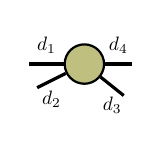
\begin{tikzpicture}[baseline=-0.5ex]
    \tikzset{tensor/.style = {minimum size = 0.5cm,shape = circle,thick,draw=black,inner sep = 0pt}, edge/.style = {thick,line width=.4mm},every loop/.style={}}
    \def\x{6}
    \def\y{0}   \node[tensor,fill=green!50!red!50!white] (T) at (\x+1,\y) {$\At$};
    \draw[edge] (T) -- (\x+0.3,0) node [midway,above] {\scalebox{0.7}{\dimcolor{$d_1$}}};
    \draw[edge] (T) -- (\x+1.6,0) node [midway,above] {\scalebox{0.7}{\dimcolor{$d_4$}}};;
    \draw[edge] (T) -- (\x+0.4,-0.3) node [midway, below] {\scalebox{0.7}{\dimcolor{$d_2$}}};
    \draw[edge] (T) -- (\x+1.5,-0.4)node [midway, below] {\scalebox{0.7}{\dimcolor{$d_3$}}};
\end{tikzpicture}\right)_{(\{1,2\})}
&=
\left(\begin{tikzpicture}[baseline=\baseline]
    \tikzset{tensor/.style = {minimum size = 0.5cm,shape = circle,thick,draw=black,inner sep = 0pt}, edge/.style   = {thick,line width=.4mm},every loop/.style={}}
    \def\y{0}
    \def\x{0}
  \node[tensor,fill=red!50!white] (A) at (\x,\y){\scalebox{0.85}{$\Ab_1$}};
  \node[tensor,fill=blue!50!white] (B) at (\x+1,\y){$\Ab_2$};
   \node[tensor,fill=red!20!white] (C) at (\x+2,\y){$\Ab_3$};
    \node[tensor,fill=blue!20!white] (D) at (\x+3,\y){$\Ab_4$};
    \draw  node[fill = black,circle,inner sep=0pt,minimum size=4pt] (m) at (\x+1.5,\y+0.7) {};
    \draw[edge] (A) -- (m)node [midway, above] {\scalebox{0.7}{\dimcolor{$R$}}} ;
    \draw[edge] (B) -- (m);
    \draw[edge] (C) -- (m);
    \draw[edge] (D) -- (m)node [midway, above] {\scalebox{0.7}{\dimcolor{$R$}}};
    \draw[edge](A) -- (\x,\y-0.7)node [midway,left] {\scalebox{0.7}{\dimcolor{$d_1$}}};
    \draw[edge](B) -- (\x+1,\y-0.7)node [midway,left] {\scalebox{0.7}{\dimcolor{$d_2$}}};
    \draw[edge](C) -- (\x+2,\y-0.7)node [midway,left] {\scalebox{0.7}{\dimcolor{$d_3$}}};
    \draw[edge](D) -- (\x+3,\y-0.7) node [midway,left] {\scalebox{0.7}{\dimcolor{$d_4$}}};
\end{tikzpicture}\right)_{(\{1,2\})}\\
&=
\begin{tikzpicture}[baseline=\baseline]
    \tikzset{tensor/.style = {minimum size = 0.5cm,shape = circle,thick,draw=black,inner sep = 0pt}, edge/.style   = {thick,line width=.4mm},every loop/.style={}}
    \def\y{0}
    \def\x{0}
  \node[tensor,fill=red!50!white] (A) at (\x,\y){\scalebox{0.85}{$\Ab_1$}};
  \node[tensor,fill=blue!50!white] (B) at (\x+1,\y){$\Ab_2$};
   \node[tensor,fill=red!20!white] (C) at (\x+2,\y){$\Ab_3$};
    \node[tensor,fill=blue!20!white] (D) at (\x+3,\y){$\Ab_4$};
    \draw  node[fill = black,circle,inner sep=0pt,minimum size=4pt] (m1) at (\x+0.5,\y+0.7) {};
    \draw  node[fill = black,circle,inner sep=0pt,minimum size=4pt] (m2) at (\x+2.5,\y+0.7) {};
    \draw[edge](A) -- (\x,\y-0.65) -- (\x+0.5,\y-0.65) -- (\x+0.5,\y-1);
    \draw[edge](B) -- (\x+1,\y-0.65) -- (\x+0.6,\y-0.65) -- (\x+0.6,\y-1);
    \draw[edge](C) -- (\x+2,\y-0.65) -- (\x+2.5,\y-0.65) -- (\x+2.5,\y-1);
    \draw[edge](D) -- (\x+3,\y-0.65) -- (\x+2.6,\y-0.65) -- (\x+2.6,\y-1);
    \node[draw=none] at (\x+0.55,\y-1.15){\scalebox{0.7}{\dimcolor{$d_1d_2$}}};
    \node[draw=none] at (\x+2.55,\y-1.15){\scalebox{0.7}{\dimcolor{$d_3d_4$}}};
    \draw[dotted] (\x+1.5,\y+1.5) -- (\x+1.5,\y-0.7);
    \draw[edge](A) -- (m1)node [midway,left] {\scalebox{0.7}{\dimcolor{$R$}}};;
    \draw[edge](B) -- (m1)node [midway,right] {\scalebox{0.7}{\dimcolor{$R$}}};
    \draw[edge](C) -- (m2)node [midway,left] {\scalebox{0.7}{\dimcolor{$R$}}};
    \draw[edge](D) -- (m2)node [midway,right] {\scalebox{0.7}{\dimcolor{$R$}}};
    \draw[edge](m1)--(m2)node [near start, above] {\scalebox{0.7}{\dimcolor{$R$}}};
\end{tikzpicture}.
\end{align*}
\item  张量 $\At \in \RR^{d_1\times \cdots \times d_N}$ 的 CP 秩有一个容易得到的上界~\citep{kolda2009tensor}
$$\cprank(\At)\leq \min_{n\in [N]} \prod_{i\neq n} d_i.$$
\item 对二阶张量 $\Ab\in\RR^{d_1\times d_2}$，CP 秩恰好对应经典的矩阵秩概念。
\item CP 分解 $\At = \CP{\Ab,\Bb,\Cb}$ 可用克罗内克 $\delta$ 写为
$$\At_{i,j,k} = \sum_{r_1,r_2,r_3}\delta_{r_1,r_2,r_3}\Ab_{i,r_1}\Bb_{j,r_2}\Cb_{k,r_3},$$
也可借助模 $n$ 乘积写成（见~\ref{par:mode-n-tensor-product}）
$$\At = \It\ttm{1}\Ab\ttm{2}\Bb\ttm{3}\Cb$$
其中 $\It$ 为三阶复制张量。
\item 二阶张量（矩阵）的秩在域 $\RR$ 与 $\CC$ 上是相同的。但对高阶张量（阶数 $N\geq3$ 的 $N$ 阶张量），秩会随分解所用的域而改变~\citep{kruskal1989rank}。
\item 对一个 $N$ 阶、每维长度均为 $d$ 的张量（$d_1 = \dots = d_N = d$），其 CP 分解的参数个数为 $NdR$，而完整张量需要 $d^N$ 个参数。若 $R$ 很小，参数个数便可大幅减少。
\end{enumerate}
\end{remark}
下面的命题说明：张量 CP 分解的模 $n$ 矩阵化可以用 Khatri-Rao 积来表达。
\begin{proposition}
设 $\At\in\RR^{d_1\times d_2\times\dots\times d_N}$。若 $\At=\CP{\Ab_1,\Ab_2,\dots,\Ab_N}$，则
$$\At_{(n)}=\Ab_n\left(\Ab_1\krao\dots\krao\Ab_{(n-1)}\krao\Ab_{(n+1)}\krao\dots\krao\Ab_N\right)^\ts.$$
\begin{proof}
取 $N=3$ 且 $n=1$，
\begin{align*}
\At_{(1)}
&=
\left(\begin{tikzpicture}[baseline=\baseline]
    \tikzset{tensor/.style = {minimum size = 0.5cm,shape = circle,thick,draw=black,inner sep = 0pt}, edge/.style  = {thick,line width=.4mm},every loop/.style={}}
    \def\y{0}
    \def\x{0}
    \node[tensor,fill=green!50!red!50!white] (At) at (\x,\y){\scalebox{0.85}{$\At$}};
    \draw[edge] (\x+0.25,\y) -- (\x+0.6,\y)  node [midway,above] {\scalebox{0.7}{\dimcolor{$d_2$}}};
    \draw[edge] (\x-0.25,\y) -- (\x-0.6,\y)  node [midway,above] {\scalebox{0.7}{\dimcolor{$d_1$}}};
    \draw[edge] (\x,\y-0.25) -- (\x,\y-0.7)  node [midway,left] {\scalebox{0.7}{\dimcolor{$d_3$}}};
    \end{tikzpicture}\right)_{(1)}
=
\left(\begin{tikzpicture}[baseline=\baseline]
    \tikzset{tensor/.style = {minimum size = 0.5cm,shape = circle,thick,draw=black,inner sep = 0pt}, edge/.style   = {thick,line width=.4mm},every loop/.style={}}
    \def\y{0}
    \def\x{0}
  \node[tensor,fill=red!50!white] (A1) at (\x,\y){\scalebox{0.85}{$\Ab_1$}};
  \node[tensor,fill=blue!50!white] (A2) at (\x+1,\y){$\Ab_2$};
   \node[tensor,fill=blue!20!white] (A3) at (\x+2,\y){$\Ab_3$};
    \draw  node[fill = black,circle,inner sep=0pt,minimum size=4pt] (m) at (\x+1,\y+1) {};
    \draw[edge] (A1) -- (m) node [midway,left] {\scalebox{0.7}{\dimcolor{$R$}}};
    \draw[edge] (A2) -- (m)node [midway,left=-0.05cm] {\scalebox{0.7}{\dimcolor{$R$}}};
    \draw[edge] (A3) -- (m)node [midway,right] {\scalebox{0.7}{\dimcolor{$R$}}};
    \draw[edge](A1) -- (\x,\y-0.7)node [midway,left] {\edgelabel{$d_1$}};
    \draw[edge](A2) -- (\x+1,\y-0.7)node [midway,left] {\edgelabel{$d_2$}};
    \draw[edge](A3) -- (\x+2,\y-0.7)node [midway,left] {\edgelabel{$d_3$}};
\end{tikzpicture}\right)_{(1)}\\
&=
\begin{tikzpicture}[baseline=\baseline]
    \tikzset{tensor/.style = {minimum size = 0.5cm,shape = circle,thick,draw=black,inner sep = 0pt}, edge/.style   = {thick,line width=.4mm},every loop/.style={}}
    \def\y{0}
    \def\x{0}
    \node[tensor,fill=green!50!red!50!white] (At) at (\x,\y){\scalebox{0.85}{$\At$}};
    \draw[edge] (\x-0.25,\y) -- (\x-0.6,\y)  node [midway,above] {\scalebox{0.7}{\dimcolor{$d_1$}}};
    \draw[edge] (\x+0.2,\y+0.15) -- (\x+0.5,\y+0.15)-- (\x+0.5,\y+0.05) -- (\x+1,\y+0.05) node [midway,above]
    {\scalebox{0.7}{\dimcolor{$d_2$}}};
    \draw[edge] (\x+0.2,\y-0.15) -- (\x+0.5,\y-0.15)-- (\x+0.5,\y-0.05)-- (\x+1,\y-0.05) node [midway,below]
    {\scalebox{0.7}{\dimcolor{$d_3$}}};
    \end{tikzpicture}
=
\begin{tikzpicture}[baseline=\baseline]
    \tikzset{tensor/.style = {minimum size = 0.5cm,shape = circle,thick,draw=black,inner sep = 0pt}, edge/.style   = {thick,line width=.4mm},every loop/.style={}}
    \def\y{0}
    \def\x{0}
    \node[tensor,fill=red!50!white] (A1) at (\x,\y){\scalebox{0.85}{$\Ab_1$}};
    \node[tensor,fill=blue!50!white] (A2) at (\x+1.7,\y+0.7){$\Ab_2$};
    \node[tensor,fill=blue!20!white] (A3) at (\x+1.7,\y-0.7){$\Ab_3$};
    \draw  node[fill = black,circle,inner sep=0pt,minimum size=4pt] (m) at (\x+1,\y) {};
    \draw[edge] (A1) -- (m) node [very near end,above] {\scalebox{0.7}{\dimcolor{$R$}}};
    \draw[edge] (A2) -- (m);
    \draw[edge] (A3) -- (m);
    \draw[edge] (A1) -- (\x-0.7,\y) node [midway,above] {\scalebox{0.7}{\dimcolor{$d_1$}}};
    \draw[edge] (A2) -- (\x+2.5,\y+0.7) -- (\x+2.5,\y+0.05)-- (\x+3,\y+0.05) node [midway,above]
    {\scalebox{0.7}{\dimcolor{$d_2$}}};
    \draw[edge] (A3) -- (\x+2.5,\y-0.7) -- (\x+2.5,\y-0.05) -- (\x+3,\y-0.05) node [midway,below]
    {\scalebox{0.7}{\dimcolor{$d_3$}}};
    \end{tikzpicture}
=
\Ab_1(\Ab_2\krao\Ab_3)^\ts.
\end{align*}
\end{proof}
\end{proposition}


\subsection{Tucker 分解}
Tucker 分解 \cite{tucker1966some} 将一个 $N$ 阶张量
分解为较小的张量与因子矩阵。在这种分解中，较小的张量称为
\emph{核心张量}（core tensor）。Tucker 分解由核心张量与因子矩阵之间的
$N$ 个模 $n$ 乘积构成
（例如参见第~\ref{sec:product}~节）。

设 $\Tt \in \RR^{d_1 \times \dots \times d_N}$。$\Tt$ 的一个 Tucker 分解
由下式给出
\[
    \Tt
    = \Gt \times_1 \Ub_1 \times_2 \Ub_2\times_3 \dots \times_N \Ub_N,
\]
其中 $\Gt \in \RR^{R_1 \times \dots \times R_N}$ 为核心张量，
而 $\Ub_i \in \RR^{d_i \times R_i}$（$i \in [N]$）为因子矩阵。
该 $N$ 元组 $(R_1,\dots,R_N)$ 称为此 Tucker
分解的\emph{秩}。

四阶张量 $\Tt\in\RR^{d_1\times\cdots \times d_4}$ 的 Tucker 分解可用张量网络记法表示如下。
$$
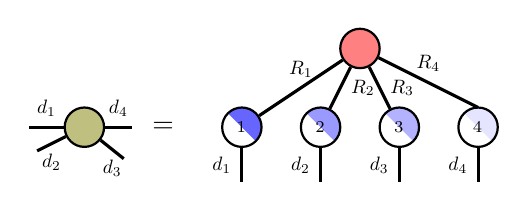
\begin{tikzpicture}[baseline=-0.5ex]
    \tikzset{tensor/.style = {minimum size = 0.5cm,shape = circle,thick,draw=black,inner sep = 0pt}, edge/.style = {thick,line width=.4mm},every loop/.style={}}
    \def\x{6}
    \def\y{0}   \node[tensor,fill=green!50!red!50!white] (T) at (\x+1,\y) {$\Tt$};
    \draw[edge] (T) -- (\x+0.3,0) node [midway,above] {\scalebox{0.7}{\dimcolor{$d_1$}}};
    \draw[edge] (T) -- (\x+1.6,0) node [midway,above] {\scalebox{0.7}{\dimcolor{$d_4$}}};;
    \draw[edge] (T) -- (\x+0.4,-0.3) node [midway, below] {\scalebox{0.7}{\dimcolor{$d_2$}}};
    \draw[edge] (T) -- (\x+1.5,-0.4)node [midway, below] {\scalebox{0.7}{\dimcolor{$d_3$}}};
    \node[draw = none] at (\x+2,0){$=$};
\node[tensor,fill=red!50!white] (G) at (\x+4.5,\y+1) {$\Gt$};
    \node[tensor, path picture={
    \fill[fill=blue!60!white](path picture bounding box.south east)
    -- 
    (path picture bounding box.north west) --
    (path picture bounding box.north east) -- cycle;
    }, shift={(\x+3,\y)}] (U_1) {\scalebox{0.85}{$\Ub_1$}};
    \node[tensor, path picture={
    \fill[fill=blue!40!white](path picture bounding box.south east)
    -- 
    (path picture bounding box.north west) --
    (path picture bounding box.north east) -- cycle;
    }, shift={(\x+4,\y)}] (U_2) {\scalebox{0.85}{$\Ub_2$}};
    \node[tensor, path picture={
    \fill[fill=blue!30!white](path picture bounding box.south east)
    -- 
    (path picture bounding box.north west) --
    (path picture bounding box.north east) -- cycle;
    }, shift={(\x+5,\y)}] (U_3) {\scalebox{0.85}{$\Ub_3$}};
    \node[tensor, path picture={
    \fill[fill=blue!10!white](path picture bounding box.south east)
    -- 
    (path picture bounding box.north west) --
    (path picture bounding box.north east) -- cycle;
    }, shift={(\x+6,\y)}] (U_4) {\scalebox{0.85}{$\Ub_4$}};
    \draw[edge] (G) -- (U_1) node [midway, above] {\scalebox{0.7}{\dimcolor{$R_1$}}};
    \draw[edge] (G) -- (U_2) node [midway, right] {\scalebox{0.7}{\dimcolor{$R_2$}}};
    \draw[edge] (G) -- (U_3) node [midway, right] {\scalebox{0.7}{\dimcolor{$R_3$}}};
    \draw[edge] (G) -- (\x+6,\y+0.25) node [midway, above] {\scalebox{0.7}{\dimcolor{$R_4$}}};
    \draw[edge] (U_1) -- (\x+3,\y-0.7) node [midway, left] {\scalebox{0.7}{\dimcolor{$d_1$}}};
    \draw[edge] (U_2) -- (\x+4,\y-0.7) node [midway, left] {\scalebox{0.7}{\dimcolor{$d_2$}}};
    \draw[edge] (U_3) -- (\x+5,\y-0.7) node [midway, left] {\scalebox{0.7}{\dimcolor{$d_3$}}};
    \draw[edge] (U_4) -- (\x+6,\y-0.7) node [midway, left] {\scalebox{0.7}{\dimcolor{$d_4$}}};
\end{tikzpicture}.
$$


不难证明，因子矩阵
$\Ub_i \in \RR^{d_i \times R_i}$ 总可以取为酉矩阵（见下方注记~\ref{rem:tuckers}
中的第~\ref{item:Tucker_orth}~条）。


\paragraph{多重线性秩（Multi-linear rank）} 张量 $\Tt$ 的\emph{多重线性（或 Tucker）秩}\footnote{注意区分 Tucker \emph{分解}的秩 $(R_1,\dots,R_n)$ 与
张量 $\Tt$ 的（Tucker）多重线性秩：前者由
$\Tt = \Gt \times_1 \Ub_1 \times_2 \dots \times_N \Ub_N$ 中核心张量 $\Gt$ 的尺寸给出，
后者定义为满足条件的最小元组。} 是使得
$\Tt$ 存在秩 $(R_1,\dots,R_N)$ 的分解的所有元组中最小的
$(R_1,\dots,R_N)$。由于整数元组上只有
偏序关系，人们会问这一秩的概念是否良定义。
下面的命题说明它确实是良定义的。

\begin{proposition}
设 $\Tt = \Gt \times_1 \Ub_1 \times_2 \Ub_2\times_3\dots \times_N \Ub_N$ 与
$\Tt = \tilde\Gt \times_1 \tilde\Ub_1 \times_2 \tilde\Ub_2\times_3 \dots \times_N \tilde\Ub_N$ 是同一
张量 $\Tt$ 的两个 Tucker 分解，其秩分别为 $(R_1,R_2,\dots, R_n)$ 与
$(\tilde R_1,\tilde R_2,\dots,\tilde R_n)$。则 $\Tt$ 存在秩为 $(\min(R_1,\tilde R_1), \min(R_2,\tilde R_2), \dots, \min(R_N,\tilde R_N))$ 的 Tucker 分解。
\end{proposition}
\begin{proof}
设 $N=3$。对 $\Tt$ 的两个 Tucker 分解分别应用模 $1$ 展开与定理~\ref{thm: matricization-rank}，可得下列结果：
\begin{align*}
    \rank\left(\begin{tikzpicture}[baseline=\baseline]
    \tikzset{tensor/.style = {minimum size = 0.5cm,shape = circle,thick,draw=black,inner sep = 0pt}, edge/.style  = {thick,line width=.4mm},every loop/.style={}}
    \def\y{0}
    \def\x{0}
    \node[tensor,fill=green!50!red!50!white] (Tt) at (\x,\y){\scalebox{0.85}{$\Tt$}};
    \draw[edge] (\x+0.25,\y) -- (\x+0.6,\y)  node [midway,above] {\scalebox{0.7}{\dimcolor{$d_2$}}};
    \draw[edge] (\x-0.25,\y) -- (\x-0.6,\y)  node [midway,above] {\scalebox{0.7}{\dimcolor{$d_1$}}};
    \draw[edge] (\x,\y-0.25) -- (\x,\y-0.7)  node [midway,left] {\scalebox{0.7}{\dimcolor{$d_3$}}};
    \end{tikzpicture}\right)_{(1)}
=
\rank(\begin{tikzpicture}[baseline=\baseline]
    \tikzset{tensor/.style = {minimum size = 0.5cm,shape = circle,thick,draw=black,inner sep = 0pt}, edge/.style  = {thick,line width=.4mm},every loop/.style={}}
    \def\y{0}
    \def\x{0}
    \node[tensor,fill=green!50!red!50!white] (Tt) at (\x,\y){\scalebox{0.85}{$\Tt$}};
    \draw[edge] (Tt) -- (\x-0.6,\y)  node [midway,above] {\scalebox{0.7}{\dimcolor{$d_1$}}};
    \draw[edge] (Tt) -- (\x+0.6,\y)  node [midway,above] {\scalebox{0.7}{\dimcolor{$d_2$}}};    \draw[edge] (Tt) -- (\x+0.6,\y)  node [midway,above] {\scalebox{0.7}{\dimcolor{$d_2$}}};
    \draw[edge] (\x+0.25,\y-0.1) -- (\x+0.6,\y-0.1)  node [midway,below] {\scalebox{0.7}{\dimcolor{$d_3$}}};
\end{tikzpicture})
=
\rank\left(\begin{tikzpicture}[baseline=\baseline]
    \tikzset{tensor/.style = {minimum size = 0.5cm,shape = circle,thick,draw=black,inner sep = 0pt}, edge/.style   = {thick,line width=.4mm},every loop/.style={}}
    \def\y{0}
    \def\x{0}
    \node[tensor,fill=blue!60!white] (U_1) at (\x,\y){\scalebox{0.85}{$\Ub_1$}};
    \node[tensor,fill=blue!30!white] (U_2) at (\x+2.7,\y+0.7){$\Ub_2$};
    \node[tensor,fill=blue!10!white] (U_3) at (\x+2.7,\y-0.7){$\Ub_3$};
    \node[tensor,fill=red!60!white] (m) at (\x+1,\y) {$\Gt$}; 
     \draw[edge] (\x+1.2,\y+0.15) -- (\x+1.5,\y+0.15)-- (\x+1.5,\y+0.05) -- (\x+2,\y+0.05) node [midway,above]
    {\scalebox{0.7}{\dimcolor{$R_2$}}};
    \draw[edge] (\x+1.2,\y-0.15) -- (\x+1.5,\y-0.15)-- (\x+1.5,\y-0.05)-- (\x+2,\y-0.05) node [midway,below]
    {\scalebox{0.7}{\dimcolor{$R_3$}}};
    \draw[edge] (U_1) -- (m) node [midway,above] {\scalebox{0.7}{\dimcolor{$R_1$}}};
    \draw[edge] (U_1) -- (\x-0.7,\y) node [midway,above] {\scalebox{0.7}{\dimcolor{$d_1$}}};
    \draw[edge](\x+2,\y-0.05) -- (\x+2,\y-0.7) -- (U_3);
    \draw[edge](\x+2,\y+0.05) -- (\x+2,\y+0.7) -- (U_2);
    \draw[edge] (U_2) -- (\x+3.5,\y+0.7) -- (\x+3.5,\y+0.05)-- (\x+4,\y+0.05) node [midway,above]
    {\scalebox{0.7}{\dimcolor{$d_2$}}};
    \draw[edge] (U_3) -- (\x+3.5,\y-0.7) -- (\x+3.5,\y-0.05) -- (\x+4,\y-0.05) node [midway,below]
    {\scalebox{0.7}{\dimcolor{$d_3$}}};
    \draw[dotted] (\x+0.45,\y+1) -- (\x+0.45,\y-1);
    \end{tikzpicture}\right)\leq R_1,
\end{align*}
同时又有
\begin{align*}
    \rank\left(\begin{tikzpicture}[baseline=\baseline]
    \tikzset{tensor/.style = {minimum size = 0.5cm,shape = circle,thick,draw=black,inner sep = 0pt}, edge/.style  = {thick,line width=.4mm},every loop/.style={}}
    \def\y{0}
    \def\x{0}
    \node[tensor,fill=green!50!red!50!white] (Tt) at (\x,\y){\scalebox{0.85}{$\Tt$}};
    \draw[edge] (\x+0.25,\y) -- (\x+0.6,\y)  node [midway,above] {\scalebox{0.7}{\dimcolor{$d_2$}}};
    \draw[edge] (\x-0.25,\y) -- (\x-0.6,\y)  node [midway,above] {\scalebox{0.7}{\dimcolor{$d_1$}}};
    \draw[edge] (\x,\y-0.25) -- (\x,\y-0.7)  node [midway,left] {\scalebox{0.7}{\dimcolor{$d_3$}}};
    \end{tikzpicture}\right)_{(1)}
=
\rank(\begin{tikzpicture}[baseline=\baseline]
    \tikzset{tensor/.style = {minimum size = 0.5cm,shape = circle,thick,draw=black,inner sep = 0pt}, edge/.style  = {thick,line width=.4mm},every loop/.style={}}
    \def\y{0}
    \def\x{0}
    \node[tensor,fill=green!50!red!50!white] (Tt) at (\x,\y){\scalebox{0.85}{$\Tt$}};
    \draw[edge] (Tt) -- (\x-0.6,\y)  node [midway,above] {\scalebox{0.7}{\dimcolor{$d_1$}}};
    \draw[edge] (Tt) -- (\x+0.6,\y)  node [midway,above] {\scalebox{0.7}{\dimcolor{$d_2$}}};    \draw[edge] (Tt) -- (\x+0.6,\y)  node [midway,above] {\scalebox{0.7}{\dimcolor{$d_2$}}};
    \draw[edge] (\x+0.25,\y-0.1) -- (\x+0.6,\y-0.1)  node [midway,below] {\scalebox{0.7}{\dimcolor{$d_3$}}};
\end{tikzpicture})
=
\rank\left(\begin{tikzpicture}[baseline=\baseline]
    \tikzset{tensor/.style = {minimum size = 0.5cm,shape = circle,thick,draw=black,inner sep = 0pt}, edge/.style   = {thick,line width=.4mm},every loop/.style={}}
    \def\y{0}
    \def\x{0}
    \node[tensor,fill=red!60!blue!20!white] (U_1) at (\x,\y){\scalebox{0.85}{$\tilde{\Ub}_1$}};
    \node[tensor,fill=red!30!blue!50!white] (U_2) at (\x+2.7,\y+0.7){$\tilde{\Ub}_2$};
    \node[tensor,fill=red!20!blue!40!white] (U_3) at (\x+2.7,\y-0.7){$\tilde{\Ub}_3$};
    \node[tensor,fill=red!40!white] (m) at (\x+1,\y) {$\tilde{\Gt}$}; 
     \draw[edge] (\x+1.2,\y+0.15) -- (\x+1.5,\y+0.15)-- (\x+1.5,\y+0.05) -- (\x+2,\y+0.05) node [midway,above]
    {\scalebox{0.7}{\dimcolor{$\tilde{R}_2$}}};
    \draw[edge] (\x+1.2,\y-0.15) -- (\x+1.5,\y-0.15)-- (\x+1.5,\y-0.05)-- (\x+2,\y-0.05) node [midway,below]
    {\scalebox{0.7}{\dimcolor{$\tilde{R}_3$}}};
    \draw[edge] (U_1) -- (m) node [midway,above] {\scalebox{0.7}{\dimcolor{$\tilde{R_1}$}}};
    \draw[edge] (U_1) -- (\x-0.7,\y) node [midway,above] {\scalebox{0.7}{\dimcolor{$d_1$}}};
    \draw[edge](\x+2,\y-0.05) -- (\x+2,\y-0.7) -- (U_3);
    \draw[edge](\x+2,\y+0.05) -- (\x+2,\y+0.7) -- (U_2);
    \draw[edge] (U_2) -- (\x+3.5,\y+0.7) -- (\x+3.5,\y+0.05)-- (\x+4,\y+0.05) node [midway,above]
    {\scalebox{0.7}{\dimcolor{$d_2$}}};
    \draw[edge] (U_3) -- (\x+3.5,\y-0.7) -- (\x+3.5,\y-0.05) -- (\x+4,\y-0.05) node [midway,below]
    {\scalebox{0.7}{\dimcolor{$d_3$}}};
    \draw[dotted] (\x+0.45,\y+1) -- (\x+0.45,\y-1);
    \end{tikzpicture}\right)\leq \tilde{R}_1,
\end{align*}
因此，$\rank\left(\begin{tikzpicture}[baseline=\baseline]
    \tikzset{tensor/.style = {minimum size = 0.5cm,shape = circle,thick,draw=black,inner sep = 0pt}, edge/.style  = {thick,line width=.4mm},every loop/.style={}}
    \def\y{0}
    \def\x{0}
    \node[tensor,fill=green!50!red!50!white] (Tt) at (\x,\y){\scalebox{0.85}{$\Tt$}};
    \draw[edge] (\x+0.25,\y) -- (\x+0.6,\y)  node [midway,above] {\scalebox{0.7}{\dimcolor{$d_2$}}};
    \draw[edge] (\x-0.25,\y) -- (\x-0.6,\y)  node [midway,above] {\scalebox{0.7}{\dimcolor{$d_1$}}};
    \draw[edge] (\x,\y-0.25) -- (\x,\y-0.7)  node [midway,left] {\scalebox{0.7}{\dimcolor{$d_3$}}};
\end{tikzpicture}\right)_{(1)}\leq\min(R_1,\tilde{R}_1)$。 
对 $n=2,3$ 同样推理即知，$\Tt$ 存在秩为 $(\min(R_1,\tilde{R}_1),\min(R_2,\tilde{R}_2),\min(R_3,\tilde{R}_3))$ 的 Tucker 分解。
\end{proof}

\paragraph{计算 Tucker 分解。} 与计算起来是 NP 难的 CP 分解不同，求出一个精确的 Tucker 分解（特别是具有最小多重线性秩的那个）可以在多项式时间内通过逐次 SVD 完成。 

Tucker 分解算法的基本思路，是在模 $n$ 上独立于其余各模，求出
$R_n$ 个主导的左奇异向量。该算法称为 \textit{高阶奇异值分解（Higher-Order SVD, HOSVD）}~\citep{de2000multilinear}，其流程画在下面。 为简单起见，我们以 $N=4$ 为例演示这一过程：
\begin{align*}
    &\begin{tikzpicture}[baseline=\baseline]
    \tikzset{tensor/.style = {minimum size = 0.5cm,shape = circle,thick,draw=black,inner sep = 0pt}, edge/.style = {thick,line width=.4mm},every loop/.style={}}
    \def\x{0}
    \def\y{0}
    \node[tensor,fill=green!50!red!50!white] (A) at (\x-5.5,\y){\scalebox{0.85}{$\Tt$}};
    \draw[edge] (A) -- (\x-5.5,\y+0.75) node [midway,left]
    {\scalebox{0.7}{\dimcolor{$d_1$}}};
    \draw[edge] (A) -- (\x-5.5,\y-0.75) node [midway,left]
    {\scalebox{0.7}{\dimcolor{$d_3$}}};
    \draw[edge] (\x-5.75,\y+0.05) -- (\x-6.2,\y-0.3) node [midway,above]
    {\scalebox{0.7}{\dimcolor{$d_2$}}};
    \draw[edge] (\x-5.25,\y+0.05) -- (\x-4.7,\y-0.3) node [midway,above]
    {\scalebox{0.7}{\dimcolor{$d_4$}}};
    \node[draw=none] at (\x-3,\y){$\underrightarrow{\text{mode-1 matricization}}$};
    \node[tensor,fill=green!50!red!50!white] (A) at (\x-0.5,\y){\scalebox{0.85}{$\Tb$}};
    \draw[edge] (\x-0.35,\y+0.2) -- (\x,\y+0.2) --(\x,\y+0.1) -- (\x
    +0.35,\y+0.1) node [midway,above]
    {\scalebox{0.7}{\dimcolor{$d_2$}}};
    \draw[edge] (\x-0.35,\y-0.2) -- (\x,\y-0.2) -- (\x,\y-0.1) -- (\x+0.35,\y-0.1) node [midway,below]
    {\scalebox{0.7}{\dimcolor{$d_4$}}};
     \draw[edge] (A) -- (\x+0.35,\y)node [right]
    {\scalebox{0.7}{\dimcolor{$d_3$}}};
     \draw[edge] (A) -- (\x-1.25,\y) node [midway,above]
    {\scalebox{0.7}{\dimcolor{$d_1$}}};
    \node[draw=none] at (\x+1,\y){$\rightarrow$};
    \node[tensor, path picture={
    \fill[fill=blue!50!white](path picture bounding box.south east)
        -- 
    (path picture bounding box.north west) --
    (path picture bounding box.north east) -- cycle;
    }, shift={(\x+1.5,\y)}] (U_1) {\scalebox{0.8}{$\Ub_1$}};
    \node[tensor,fill=red!50!white] (Sigma_1) at (\x+2.5,\y){\scalebox{0.85}{$\Sigmab_1$}};
    \node[tensor, path picture={
    \fill[fill=red!60!white](path picture bounding box.south west)
        -- 
    (path picture bounding box.north east) --
    (path picture bounding box.north west) -- cycle;
    }, shift={(\x+3.5,\y)}] (V_1) {\scalebox{0.8}{$\Vb_1$}};
    \draw[edge](V_1) -- (\x+4.5,\y) node [right]{\scalebox{0.7}{\textcolor{gray}{$d_3$}}};
    \draw[edge] (U_1) -- (Sigma_1)node [midway,above]
    {\scalebox{0.7}{\dimcolor{$R_1$}}};
    \draw[edge] (U_1) -- (\x+1.5,\y-0.7)node [midway,left]
    {\scalebox{0.7}{\dimcolor{$d_1$}}};
    \draw[edge] (Sigma_1) -- (V_1) node[midway,above]    {\scalebox{0.7}{\dimcolor{$R_1$}}};
    \draw[edge] (\x+3.7,\y+0.15) -- (\x+4,\y+0.15) --(\x+4,\y+0.1) -- (\x+4.5,\y+0.1) node [midway,above]
    {\scalebox{0.7}{\dimcolor{$d_2$}}};
    \draw[edge] (\x+3.65,\y-0.2) -- (\x+4,\y-0.2) -- (\x+4,\y-0.1) -- (\x+4.5,\y-0.1) node [midway,below]
    {\scalebox{0.7}{\dimcolor{$d_4$}}};
    \node[draw=none] at (\x+5.75,\y){\text{Keep $\Ub_1$}.};
\end{tikzpicture}\\
&\begin{tikzpicture}[baseline=\baseline]
    \tikzset{tensor/.style = {minimum size = 0.5cm,shape = circle,thick,draw=black,inner sep = 0pt}, edge/.style = {thick,line width=.4mm},every loop/.style={}}
    \def\y{0}
    \def\x{0}
    \node[tensor,fill=green!50!red!50!white] (A) at (\x-2.5,\y){\scalebox{0.85}{$\Tt$}};
    \draw[edge] (A) -- (\x-2.5,\y+0.75) node [midway,left]
    {\scalebox{0.7}{\dimcolor{$d_1$}}};
    \draw[edge] (A) -- (\x-2.5,\y-0.75) node [midway,left]
    {\scalebox{0.7}{\dimcolor{$d_3$}}};
    \draw[edge] (\x-2.75,\y+0.05) -- (\x-3.2,\y-0.3) node [midway,above]
    {\scalebox{0.7}{\dimcolor{$d_2$}}};
    \draw[edge] (\x-2.25,\y+0.05) -- (\x-1.7,\y-0.3) node [midway,above]
    {\scalebox{0.7}{\dimcolor{$d_4$}}};
    \node[draw=none] at (\x,\y){$\underrightarrow{\text{mode-2 matricization}}$};
    \node[tensor,fill=green!50!red!50!white] (A) at (\x+2.5,\y){\scalebox{0.85}{$\Tb$}};
    \draw[edge] (A) -- (\x+1.75,\y) node [midway,above]
    {\scalebox{0.7}{\dimcolor{$d_2$}}};
    \draw[edge] (A) -- (\x+3.35,\y)node [right]
    {\scalebox{0.7}{\dimcolor{$d_3$}}};
    \draw[edge] (\x+2.65,\y+0.2) -- (\x+3,\y+0.2) -- (\x+3,\y+0.1) -- (\x+3.35,\y+0.1)node [midway,above]
    {\scalebox{0.7}{\dimcolor{$d_1$}}};
    \draw[edge] (\x+2.65,\y-0.2) -- (\x+3,\y-0.2) -- (\x+3,\y-0.1) -- (\x+3.35,\y-0.1)node [midway,below]
    {\scalebox{0.7}{\dimcolor{$d_4$}}};
    \node[draw=none] at (\x+4,\y){$\rightarrow$};
    \node[tensor, path picture={
    \fill[fill=blue!40!white](path picture bounding box.south east)
        -- 
    (path picture bounding box.north west) --
    (path picture bounding box.north east) -- cycle;
    }, shift={(\x+4.5,\y)}] (U_2) {\scalebox{0.8}{$\Ub_2$}};
    \node[tensor,fill=red!40!white] (Sigma_2) at (\x+5.5,\y){\scalebox{0.85}{$\Sigmab_2$}};
    \node[tensor, path picture={
    \fill[fill=red!50!white](path picture bounding box.south west)
        -- 
    (path picture bounding box.north east) --
    (path picture bounding box.north west) -- cycle;
    }, shift={(\x+6.5,\y)}] (V_2) {\scalebox{0.8}{$\Vb_2$}};
    \draw[edge](V_2) -- (\x+7.5,\y) node [right]{\scalebox{0.7}{\dimcolor{$d_3$}}};
    \draw[edge] (U_2) -- (Sigma_2)node [midway,above]
    {\scalebox{0.7}{\dimcolor{$R_2$}}};
    \draw[edge] (U_2) -- (\x+4.5,\y-0.7)node [midway,left]
    {\scalebox{0.7}{\dimcolor{$d_2$}}};
    \draw[edge] (Sigma_2) -- (V_2) node[midway,above] {\scalebox{0.7}{\dimcolor{$R_2$}}};
    \draw[edge] (\x+6.71,\y+0.15) -- (\x+7,\y+0.15) --(\x+7,\y+0.1) -- (\x+7.5,\y+0.1) node [midway,above]
    {\scalebox{0.7}{\dimcolor{$d_1$}}};
    \draw[edge] (\x+6.65,\y-0.2) -- (\x+7,\y-0.2) -- (\x+7,\y-0.1) -- (\x+7.5,\y-0.1) node [midway,below]
    {\scalebox{0.7}{\dimcolor{$d_4$}}};
    \node[draw=none] at (\x+8.75,\y){\text{Keep $\Ub_2$}.};
\end{tikzpicture}\\
&\begin{tikzpicture}[baseline=\baseline]
    \tikzset{tensor/.style = {minimum size = 0.5cm,shape = circle,thick,draw=black,inner sep = 0pt}, edge/.style = {thick,line width=.4mm},every loop/.style={}}
    \def\y{0}
    \def\x{0}
    \node[tensor,fill=green!50!red!50!white] (A) at (\x-2.5,\y){\scalebox{0.85}{$\Tt$}};
    \draw[edge] (A) -- (\x-2.5,\y+0.75) node [midway,left]
    {\scalebox{0.7}{\dimcolor{$d_1$}}};
    \draw[edge] (A) -- (\x-2.5,\y-0.75) node [midway,left]
    {\scalebox{0.7}{\dimcolor{$d_3$}}};
    \draw[edge] (\x-2.75,\y+0.05) -- (\x-3.2,\y-0.3) node [midway,above]
    {\scalebox{0.7}{\dimcolor{$d_2$}}};
    \draw[edge] (\x-2.25,\y+0.05) -- (\x-1.7,\y-0.3) node [midway,above]
    {\scalebox{0.7}{\dimcolor{$d_4$}}};
    \node[draw=none] at (\x,\y){$\underrightarrow{\text{mode-3 matricization}}$};
    \node[tensor,fill=green!50!red!50!white] (A) at (\x+2.5,\y){\scalebox{0.85}{$\Tb$}};
    \draw[edge] (A) -- (\x+1.75,\y) node [midway,above]
    {\scalebox{0.7}{\dimcolor{$d_3$}}};
    \draw[edge] (A) -- (\x+3.35,\y)node [right]
    {\scalebox{0.7}{\dimcolor{$d_2$}}};
    \draw[edge] (\x+2.65,\y+0.2) -- (\x+3,\y+0.2) -- (\x+3,\y+0.1) -- (\x+3.35,\y+0.1)node [midway,above]
    {\scalebox{0.7}{\dimcolor{$d_1$}}};
    \draw[edge] (\x+2.65,\y-0.2) -- (\x+3,\y-0.2) -- (\x+3,\y-0.1) -- (\x+3.35,\y-0.1)node [midway,below]
    {\scalebox{0.7}{\dimcolor{$d_4$}}};
    \node[draw=none] at (\x+4,\y){$\rightarrow$};
    \node[tensor, path picture={
    \fill[fill=blue!30!white](path picture bounding box.south east)
        -- 
    (path picture bounding box.north west) --
    (path picture bounding box.north east) -- cycle;
    }, shift={(\x+4.5,\y)}] (U_3) {\scalebox{0.8}{$\Ub_3$}};
    \node[tensor,fill=red!30!white] (Sigma_3) at (\x+5.5,\y){\scalebox{0.85}{$\Sigmab_3$}};
    \node[tensor, path picture={
    \fill[fill=red!40!white](path picture bounding box.south west)
        -- 
    (path picture bounding box.north east) --
    (path picture bounding box.north west) -- cycle;
    }, shift={(\x+6.5,\y)}] (V_3) {\scalebox{0.8}{$\Vb_3$}};
    \draw[edge](V_3) -- (\x+7.5,\y) node [right]{\scalebox{0.7}{\dimcolor{$d_2$}}};
    \draw[edge] (U_3) -- (Sigma_3)node [midway,above]
    {\scalebox{0.7}{\dimcolor{$R_3$}}};
    \draw[edge] (U_3) -- (\x+4.5,\y-0.7)node [midway,left]
    {\scalebox{0.7}{\dimcolor{$d_3$}}};
    \draw[edge] (Sigma_3) -- (V_3) node[midway,above] {\scalebox{0.7}{\dimcolor{$R_3$}}};
    \draw[edge] (\x+6.71,\y+0.15) -- (\x+7,\y+0.15) --(\x+7,\y+0.1) -- (\x+7.5,\y+0.1) node [midway,above]
    {\scalebox{0.7}{\dimcolor{$d_1$}}};
    \draw[edge] (\x+6.65,\y-0.2) -- (\x+7,\y-0.2) -- (\x+7,\y-0.1) -- (\x+7.5,\y-0.1) node [midway,below]
    {\scalebox{0.7}{\dimcolor{$d_4$}}};
    \node[draw=none] at (\x+8.75,\y){\text{Keep $\Ub_3$.}};
\end{tikzpicture}\\
&\begin{tikzpicture}[baseline=\baseline]
    \tikzset{tensor/.style = {minimum size = 0.5cm,shape = circle,thick,draw=black,inner sep = 0pt}, edge/.style = {thick,line width=.4mm},every loop/.style={}}
    \def\y{0}
    \def\x{0}
    \node[tensor,fill=green!50!red!50!white] (A) at (\x-2.5,\y){\scalebox{0.85}{$\Tt$}};
    \draw[edge] (A) -- (\x-2.5,\y+0.75) node [midway,left]
    {\scalebox{0.7}{\dimcolor{$d_1$}}};
    \draw[edge] (A) -- (\x-2.5,\y-0.75) node [midway,left]
    {\scalebox{0.7}{\dimcolor{$d_3$}}};
    \draw[edge] (\x-2.75,\y+0.05) -- (\x-3.2,\y-0.3) node [midway,above]
    {\scalebox{0.7}{\dimcolor{$d_2$}}};
    \draw[edge] (\x-2.25,\y+0.05) -- (\x-1.7,\y-0.3) node [midway,above]
    {\scalebox{0.7}{\dimcolor{$d_4$}}};
    \node[draw=none] at (\x,\y){$\underrightarrow{\text{mode-4 matricization}}$};
    \node[tensor,fill=green!50!red!50!white] (A) at (\x+2.5,\y){\scalebox{0.85}{$\Tb$}};
    \draw[edge] (A) -- (\x+1.75,\y) node [midway,above]
    {\scalebox{0.7}{\dimcolor{$d_4$}}};
    \draw[edge] (A) -- (\x+3.35,\y)node [right]
    {\scalebox{0.7}{\dimcolor{$d_2$}}};
    \draw[edge] (\x+2.65,\y+0.2) -- (\x+3,\y+0.2) -- (\x+3,\y+0.1) -- (\x+3.35,\y+0.1)node [midway,above]
    {\scalebox{0.7}{\dimcolor{$d_1$}}};
    \draw[edge] (\x+2.65,\y-0.2) -- (\x+3,\y-0.2) -- (\x+3,\y-0.1) -- (\x+3.35,\y-0.1)node [midway,below]
    {\scalebox{0.7}{\dimcolor{$d_3$}}};
    \node[draw=none] at (\x+4,\y){$\rightarrow$};
    \node[tensor, path picture={
    \fill[fill=blue!20!white](path picture bounding box.south east)
        -- 
    (path picture bounding box.north west) --
    (path picture bounding box.north east) -- cycle;
    }, shift={(\x+4.5,\y)}] (U_4) {\scalebox{0.8}{$\Ub_4$}};
    \node[tensor,fill=red!20!white] (Sigma_4) at (\x+5.5,\y){\scalebox{0.85}{$\Sigmab_4$}};
    \node[tensor, path picture={
    \fill[fill=red!30!white](path picture bounding box.south west)
        -- 
    (path picture bounding box.north east) --
    (path picture bounding box.north west) -- cycle;
    }, shift={(\x+6.5,\y)}] (V_4) {\scalebox{0.8}{$\Vb_4$}};
    \draw[edge](V_4) -- (\x+7.5,\y) node [right]{\scalebox{0.7}{\dimcolor{$d_2$}}};
    \draw[edge] (U_4) -- (Sigma_4)node [midway,above]
    {\scalebox{0.7}{\dimcolor{$R_4$}}};
    \draw[edge] (U_4) -- (\x+4.5,\y-0.7)node [midway,left]
    {\scalebox{0.7}{\dimcolor{$d_4$}}};
    \draw[edge] (Sigma_4) -- (V_4) node[midway,above] {\scalebox{0.7}{\dimcolor{$R_4$}}};
    \draw[edge] (\x+6.71,\y+0.15) -- (\x+7,\y+0.15) --(\x+7,\y+0.1) -- (\x+7.5,\y+0.1) node [midway,above]
    {\scalebox{0.7}{\dimcolor{$d_1$}}};
    \draw[edge] (\x+6.65,\y-0.2) -- (\x+7,\y-0.2) -- (\x+7,\y-0.1) -- (\x+7.5,\y-0.1) node [midway,below]
    {\scalebox{0.7}{\dimcolor{$d_3$}}};
    \node[draw=none] at (\x+8.75,\y){\text{Keep $\Ub_4$.}};
\end{tikzpicture}
\end{align*}
若上述所有 SVD 都是精确的，即对每个 $n$ 有 $R_n = \rank(\Tt_{(n)})$，则对所有 $n$ 均有 $\Tt \times_n \Ub_n\Ub_n^\ts = \Tt$，从而 $\Tt = \Tt\times_1\Ub_1\Ub_1^\ts\times_2\cdots\times_N\Ub_N\Ub_N^\ts$。举例来说，当 $N=4$ 时有：
$$
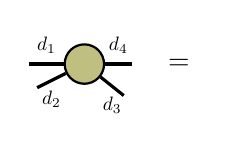
\begin{tikzpicture}[baseline=-0.5ex]
    \tikzset{tensor/.style = {minimum size = 0.5cm,shape = circle,thick,draw=black,inner sep = 0pt}, edge/.style = {thick,line width=.4mm},every loop/.style={}}
    \def\x{6}
    \def\y{0}   \node[tensor,fill=green!50!red!50!white] (T) at (\x+1,\y) {$\Tt$};
    \draw[edge] (T) -- (\x+0.3,0) node [midway,above] {\scalebox{0.7}{\dimcolor{$d_1$}}};
    \draw[edge] (T) -- (\x+1.6,0) node [midway,above] {\scalebox{0.7}{\dimcolor{$d_4$}}};;
    \draw[edge] (T) -- (\x+0.4,-0.3) node [midway, below] {\scalebox{0.7}{\dimcolor{$d_2$}}};
    \draw[edge] (T) -- (\x+1.5,-0.4)node [midway, below] {\scalebox{0.7}{\dimcolor{$d_3$}}};
    \node[draw = none] at (\x+2.2,0){$=$};
\end{tikzpicture}
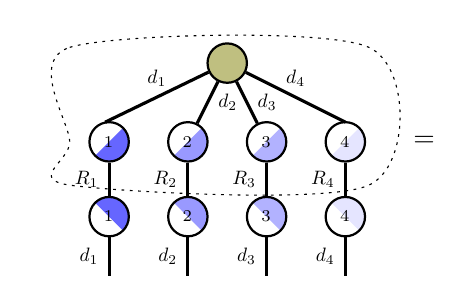
\begin{tikzpicture}[baseline=-0.5ex]
    \tikzset{tensor/.style = {minimum size = 0.5cm,shape = circle,thick,draw=black,inner sep = 0pt}, edge/.style = {thick,line width=.4mm},every loop/.style={}}
    \def\x{6}
    \def\y{0} 
    \node[tensor,fill=green!50!red!50!white] (T) at (\x+4.5,\y+1) {$\Tt$};
    \node[tensor, path picture={
    \fill[fill=blue!60!white](path picture bounding box.north east)
        -- 
    (path picture bounding box.south east) --
    (path picture bounding box.south west) -- cycle;
    }, shift={(\x+3,\y)}] (U_1) {\scalebox{0.85}{$\Ub_1$}};
    \node[tensor, path picture={
    \fill[fill=blue!60!white](path picture bounding box.south east)
        -- 
    (path picture bounding box.north east) --
    (path picture bounding box.north west) -- cycle;
    }, shift={(\x+3,\y-0.95)}] (Ut_1) {\scalebox{0.85}{$\Ub_1$}};
    \node[tensor, path picture={
    \fill[fill=blue!40!white](path picture bounding box.north east)
        -- 
    (path picture bounding box.south east) --
    (path picture bounding box.south west) -- cycle;
    }, shift={(\x+4,\y)}] (U_2) {\scalebox{0.85}{$\Ub_2$}};
    \node[tensor, path picture={
    \fill[fill=blue!40!white](path picture bounding box.south east)
        -- 
    (path picture bounding box.north east) --
    (path picture bounding box.north west) -- cycle;
    }, shift={(\x+4,\y-0.95)}] (Ut_2) {\scalebox{0.85}{$\Ub_2$}};
    \node[tensor, path picture={
    \fill[fill=blue!30!white](path picture bounding box.north east)
    -- 
    (path picture bounding box.south west) --
    (path picture bounding box.south east) -- cycle;
    }, shift={(\x+5,\y)}] (U_3) {\scalebox{0.85}{$\Ub_3$}};
    \node[tensor, path picture={
    \fill[fill=blue!30!white](path picture bounding box.south east)
        -- 
    (path picture bounding box.north east) --
    (path picture bounding box.north west) -- cycle;
    }, shift={(\x+5,\y-0.95)}] (Ut_3) {\scalebox{0.85}{$\Ub_3$}};
    \node[tensor, path picture={
    \fill[fill=blue!10!white](path picture bounding box.north east)
    -- 
    (path picture bounding box.south west) --
    (path picture bounding box.south east) -- cycle;
    }, shift={(\x+6,\y)}] (U_4) {\scalebox{0.85}{$\Ub_4$}};
    \node[tensor, path picture={
    \fill[fill=blue!10!white](path picture bounding box.south east)
        -- 
    (path picture bounding box.north east) --
    (path picture bounding box.north west) -- cycle;
    }, shift={(\x+6,\y-0.95)}] (Ut_4) {\scalebox{0.85}{$\Ub_4$}};
    \draw[edge] (T) -- (\x+2.95,\y+0.25) node [midway, above] {\scalebox{0.7}{\dimcolor{$d_1$}}};
    \draw[edge] (T) -- (U_2) node [midway, right] {\scalebox{0.7}{\dimcolor{$d_2$}}};
    \draw[edge] (T) -- (U_3) node [midway, right] {\scalebox{0.7}{\dimcolor{$d_3$}}};
    \draw[edge] (T) -- (\x+6,\y+0.25) node [midway, above] {\scalebox{0.7}{\dimcolor{$d_4$}}};
    \draw[edge] (U_1) -- (\x+3,\y-0.7) node [midway, left] {\scalebox{0.7}{\dimcolor{$R_1$}}};
    \draw[edge] (U_2) -- (\x+4,\y-0.7) node [midway, left] {\scalebox{0.7}{\dimcolor{$R_2$}}};
    \draw[edge] (U_3) -- (\x+5,\y-0.7) node [midway, left] {\scalebox{0.7}{\dimcolor{$R_3$}}};
    \draw[edge] (U_4) -- (\x+6,\y-0.7) node [midway, left] {\scalebox{0.7}{\dimcolor{$R_4$}}};
    \draw[edge] (Ut_1) -- (\x+3,\y-1.7) node [midway, left] {\scalebox{0.7}{\dimcolor{$d_1$}}};
    \draw[edge] (Ut_2) -- (\x+4,\y-1.7) node [midway, left] {\scalebox{0.7}{\dimcolor{$d_2$}}};
    \draw[edge] (Ut_3) -- (\x+5,\y-1.7) node [midway, left] {\scalebox{0.7}{\dimcolor{$d_3$}}};
    \draw[edge] (Ut_4) -- (\x+6,\y-1.7) node [midway, left] {\scalebox{0.7}{\dimcolor{$d_4$}}};
    \draw[dash pattern=on 1pt off 2pt] plot[smooth cycle] coordinates { 
    (\x+2.5,\y) 
    (\x+2.5, \y+1.2) (\x+6.3,\y+1.2) (\x+6.3, \y-0.55)  (\x+2.5,\y-0.55)};
    \node[draw = none] at (\x+7,0){$=$};
\end{tikzpicture}
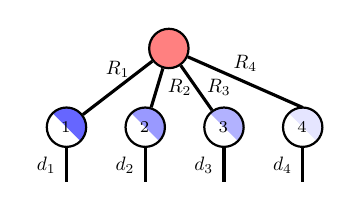
\begin{tikzpicture}[baseline=-0.5ex]
    \tikzset{tensor/.style = {minimum size = 0.5cm,shape = circle,thick,draw=black,inner sep = 0pt}, edge/.style = {thick,line width=.4mm},every loop/.style={}}
    \def\x{6}
    \def\y{0} 
    \node[tensor,fill=red!50!white] (G) at (\x+13.5,\y+1) {$\Gt$};
    \node[tensor, path picture={
    \fill[fill=blue!60!white](path picture bounding box.south east)
    -- 
    (path picture bounding box.north west) --
    (path picture bounding box.north east) -- cycle;
    }, shift={(\x+12.2,\y)}] (U_1)  {\scalebox{0.85}{$\Ub_1$}};  \node[tensor, path picture={
    \fill[fill=blue!40!white](path picture bounding box.south east)
    -- 
    (path picture bounding box.north west) --
    (path picture bounding box.north east) -- cycle;
    }, shift={(\x+13.2,\y)}] (U_2) {\scalebox{0.85}{$\Ub_2$}};
    \node[tensor, path picture={
    \fill[fill=blue!30!white](path picture bounding box.south east)
    -- 
    (path picture bounding box.north west) --
    (path picture bounding box.north east) -- cycle;
    }, shift={(\x+14.2,\y)}] (U_3) {\scalebox{0.85}{$\Ub_3$}};
        \node[tensor, path picture={
    \fill[fill=blue!10!white](path picture bounding box.south east)
    -- 
    (path picture bounding box.north west) --
    (path picture bounding box.north east) -- cycle;
    }, shift={(\x+15.2,\y)}] (U_4) {\scalebox{0.85}{$\Ub_4$}};
     \draw[edge] (U_1) -- (\x+12.2,\y-0.7) node [midway, left] {\scalebox{0.7}{\dimcolor{$d_1$}}};
    \draw[edge] (U_2) -- (\x+13.2,\y-0.7) node [midway, left] {\scalebox{0.7}{\dimcolor{$d_2$}}};
    \draw[edge] (U_3) -- (\x+14.2,\y-0.7) node [midway, left] {\scalebox{0.7}{\dimcolor{$d_3$}}};
    \draw[edge] (U_4) -- (\x+15.2,\y-0.7) node [midway, left] {\scalebox{0.7}{\dimcolor{$d_4$}}};
    \draw[edge](G) -- (U_1)node[midway,above]{\scalebox{0.7}{\dimcolor{$R_1$}}};
    \draw[edge](G) -- (U_2)node[midway,right]{\scalebox{0.7}{\dimcolor{$R_2$}}};
    \draw[edge](G) -- (U_3)node[midway,right]{\scalebox{0.7}{\dimcolor{$R_3$}}};
    \draw[edge](G) -- (\x+15.2,\y+0.25)node[midway,above]{\scalebox{0.7}{\dimcolor{$R_4$}}};
\end{tikzpicture}.
$$
其中张量 $\Gt = \Tt\ttm{1}\Ub_1^\ts\ttm{2}\dots\ttm{4}\Ub_4^\ts$。 

核心张量  $\Gt\in\RR^{R_1\times\dots\times R_4}$ 与因子矩阵 $\Ub_1,\dots,\Ub_4$ 一起构成张量 $\Tt$ 的一个 Tucker 分解。若 $\Tt$ 各矩阵化上的 SVD 全部精确，则所得的 Tucker 分解也是精确的。使用截断 SVD 时，Tucker 分解的整体逼近误差可表示为各截断 SVD 所引入误差的函数~(见~\citep{de2000multilinear})。

\paragraph{多重线性秩与矩阵化的秩}
上述算法表明：若对所有 $n$ 有 $\tilde R_n = \rank(\Tt_{(n)})$，则存在秩为 $(\tilde R_1,\dots, \tilde R_N)$ 的 Tucker 分解，这说明 $\Tt$ 的多重线性秩 $( R_1,\dots, R_N)$ 以矩阵化的秩为上界，即对所有 $n$ 有 $ R_n \leq \rank(\Tt_{(n)} )$。也容易证明，多重线性秩以矩阵化的秩为下界。事实上，设 $\T$ 的多重线性秩为 $(R_1,\dots, R_N)$，则存在秩 $(R_1,\dots, R_N)$ 的 Tucker 分解 $\Tt = \Gt\times_1\Ub_1\times_2 \dots \times_N \Ub_N$。由定理~\ref{thm: matricization-rank} 即可看出，这意味着对所有 $n$ 有 $\rank(\Tt_{(n)} )\leq  R_n$。
这就证明了如下定理。
\begin{theorem}
张量 $\Tt$ 的多重线性秩 $(R_1,R_2,\dots, R_N)$ 由其矩阵化的秩给出，即对 $n\in[N]$ 有 $R_n = \rank(\Tt_{(n)})$。
\end{theorem}


\begin{remark}\label{rem:tuckers}
这里列出 Tucker 分解以及用于计算它的高阶奇异值分解~(HOSVD) 算法的一些有趣性质。
\begin{enumerate}

\item  若 $\Tt = \Gt\ttm{1}\Ub_1\ttm{2}\dots\ttm{N-1}\Ub_{N-1}\ttm{N}\Ub_N$ 且所有 $\Ub_i$ 均正交，则 $\norm{\Tt}_F = \norm{\Gt}_F$，且 $\vectorize(\Gt) = (\Ub_1\kron\cdots\kron\Ub_N)\vectorize(\Tt)$。
事实上，当 $N=3$ 时有
\begin{align*}
(\Ub_1\kron\Ub_2\kron\Ub_3)\vectorize(\Tt) &= 
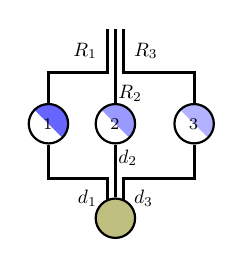
\begin{tikzpicture}[baseline=-0.5ex]
    \tikzset{tensor/.style = {minimum size = 0.5cm,shape = circle,thick,draw=black,inner sep = 0pt}, edge/.style = {thick,line width=.4mm},every loop/.style={}}
    \def\x{0}
    \def\y{0.5}   
    \node[tensor, path picture={
    \fill[fill=blue!60!white](path picture bounding box.south east)
        -- 
    (path picture bounding box.north west) --
    (path picture bounding box.north east) -- cycle;
    }, shift={(\x-0.85,\y-0.65)}] (U_1) {\scalebox{0.85}{$\Ub_1$}};
    \node[tensor, path picture={
    \fill[fill=blue!40!white](path picture bounding box.south east)
        -- 
    (path picture bounding box.north west) --
    (path picture bounding box.north east) -- cycle;
    }, shift={(\x,\y-0.65)}] (U_2) {\scalebox{0.85}{$\Ub_2$}};
    \node[tensor, path picture={
    \fill[fill=blue!30!white](path picture bounding box.south east)
        -- 
    (path picture bounding box.north west) --
    (path picture bounding box.north east) -- cycle;
    }, shift={(\x+1,\y-0.65)}] (U_3) {\scalebox{0.85}{$\Ub_3$}};
    \draw[edge] (U_1) -- (\x-0.85,\y-1.35) -- (\x-0.1,\y-1.35) -- (\x-0.1,\y-1.85) node [midway, left] {\scalebox{0.7}{\dimcolor{$d_1$}}};
    \draw[edge] (U_2) -- (\x,\y+0.55) node [very near start, right=-0.1cm] {\scalebox{0.7}{\dimcolor{$R_2$}}};
    \draw[edge] (U_3) -- (\x+1,\y-1.35) -- (\x+0.1,\y-1.35) -- (\x+0.1, \y-1.85) node [midway, right] {\scalebox{0.7}{\dimcolor{$d_3$}}};
    \draw[edge](U_1) -- (\x-0.85,\y) -- (\x-0.1,\y) -- (\x-0.1,\y+0.55)node [midway, left] {\scalebox{0.7}{\dimcolor{$R_1$}}};
    \draw[edge](U_3) -- (\x+1,\y) -- (\x+0.1,\y) -- (\x+0.1,\y+0.55)node [midway, right] {\scalebox{0.7}{\dimcolor{$R_3$}}};
    \node[tensor,fill=green!50!red!50!white](T) at (\x,\y-1.85) {$\Tt$};
    \draw[edge](U_2)--(T)node [near start, right=-0.1cm] {\scalebox{0.7}{\dimcolor{$d_2$}}};
\end{tikzpicture}
=
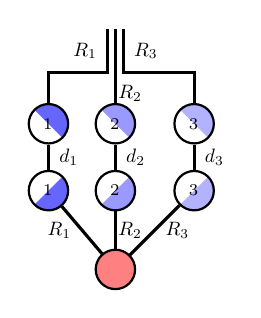
\begin{tikzpicture}[baseline=-0.5ex]
    \tikzset{tensor/.style = {minimum size = 0.5cm,shape = circle,thick,draw=black,inner sep = 0pt}, edge/.style = {thick,line width=.4mm},every loop/.style={}}
    \def\x{0}
    \def\y{1.25}   
    \node[tensor, path picture={
    \fill[fill=blue!60!white](path picture bounding box.south east)
        -- 
    (path picture bounding box.north west) --
    (path picture bounding box.north east) -- cycle;
    }, shift={(\x-0.85,\y-0.65)}] (U_1) {\scalebox{0.85}{$\Ub_1$}};
    \node[tensor, path picture={
    \fill[fill=blue!60!white](path picture bounding box.north east)
        -- 
    (path picture bounding box.south west) --
    (path picture bounding box.south east) -- cycle;
    }, shift={(\x-0.85,\y-1.5)}] (Ut_1) {\scalebox{0.85}{$\Ub_1$}};
    \node[tensor, path picture={
    \fill[fill=blue!40!white](path picture bounding box.south east)
        -- 
    (path picture bounding box.north west) --
    (path picture bounding box.north east) -- cycle;
    }, shift={(\x,\y-0.65)}] (U_2) {\scalebox{0.85}{$\Ub_2$}};
     \node[tensor, path picture={
    \fill[fill=blue!40!white](path picture bounding box.north east)
        -- 
    (path picture bounding box.south west) --
    (path picture bounding box.south east) -- cycle;
    }, shift={(\x,\y-1.5)}] (Ut_2) {\scalebox{0.85}{$\Ub_2$}};
    \node[tensor, path picture={
    \fill[fill=blue!30!white](path picture bounding box.south east)
        -- 
    (path picture bounding box.north west) --
    (path picture bounding box.north east) -- cycle;
    }, shift={(\x+1,\y-0.65)}] (U_3) {\scalebox{0.85}{$\Ub_3$}};
    \node[tensor, path picture={
    \fill[fill=blue!30!white](path picture bounding box.north east)
        -- 
    (path picture bounding box.south west) --
    (path picture bounding box.south east) -- cycle;
    }, shift={(\x+1,\y-1.5)}] (Ut_3) {\scalebox{0.85}{$\Ub_3$}};
    \draw[edge] (U_2) -- (\x,\y+0.55) node [very near start, right=-0.1cm] {\scalebox{0.7}{\dimcolor{$R_2$}}};
    \draw[edge](U_1) -- (\x-0.85,\y) -- (\x-0.1,\y) -- (\x-0.1,\y+0.55)node [midway, left] {\scalebox{0.7}{\dimcolor{$R_1$}}};
    \draw[edge](U_3) -- (\x+1,\y) -- (\x+0.1,\y) -- (\x+0.1,\y+0.55)node [midway, right] {\scalebox{0.7}{\dimcolor{$R_3$}}};
    \draw[edge](U_1)--(Ut_1)node [midway, right] {\scalebox{0.7}{\dimcolor{$d_1$}}};
    \draw[edge](U_2)--(Ut_2)node [midway, right] {\scalebox{0.7}{\dimcolor{$d_2$}}};
    \draw[edge](U_3)--(Ut_3)node [midway, right] {\scalebox{0.7}{\dimcolor{$d_3$}}};
    \node[tensor,fill=red!50!white] (G) at (\x,\y-2.5) {$\Gt$};
    \draw[edge](G)--(Ut_1)node [midway, left] {\scalebox{0.7}{\dimcolor{$R_1$}}};
    \draw[edge](G)--(Ut_2)node [midway, right=-0.1cm] {\scalebox{0.7}{\dimcolor{$R_2$}}};
    \draw[edge](G)--(Ut_3)node [midway, right] {\scalebox{0.7}{\dimcolor{$R_3$}}};
\end{tikzpicture}
=
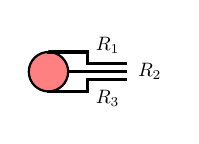
\begin{tikzpicture}[baseline=-0.5ex]
    \tikzset{tensor/.style = {minimum size = 0.5cm,shape = circle,thick,draw=black,inner sep = 0pt}, edge/.style = {thick,line width=.4mm},every loop/.style={}}
    \def\x{6}
    \def\y{0}
    \node[tensor,fill=red!50!white] (G) at (\x+4.5,\y) {$\Gt$};
    \draw[edge](G) -- (\x+5.5,\y) node [right] {\scalebox{0.7}{\dimcolor{$R_2$}}};
    \draw[edge](G) -- (\x+4.5,\y+0.25) -- (\x+5,\y+0.25) -- (\x+5,\y+0.1) -- (\x+5.5, \y+0.1) node [midway,above] {\scalebox{0.7}{\dimcolor{$R_1$}}};
    \draw[edge](G) -- (\x+4.5,\y-0.25) -- (\x+5,\y-0.25) -- (\x+5,\y-0.1) -- (\x+5.5, \y-0.1) node [midway,below] {\scalebox{0.7}{\dimcolor{$R_3$}}};
    \end{tikzpicture}
    =\vectorize(\Gt).
\end{align*}

注意到 $\Ub_1\kron\Ub_2\kron\Ub_3$ 是左正交矩阵，于是 
 $\norm{\Tt} = \norm{\vectorize(\Tt)} = \norm{(\Ub_1\kron\Ub_2\kron\Ub_3)\vectorize(\Tt)}= \norm{\vectorize(\Gt)} = \norm{\Gt}$.
    


    \item 若不对因子矩阵施加任何正交约束，并将核心张量固定为复制张量，
$
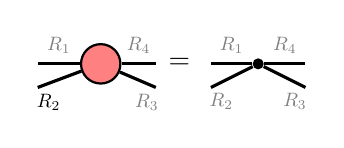
\begin{tikzpicture}[baseline=-0.5ex]
    \tikzset{tensor/.style = {minimum size = 0.5cm,shape = circle,thick,draw=black,inner sep = 0pt}, edge/.style = {thick,line width=.4mm},every loop/.style={}}
    \def\x{6}
    \def\y{0}
    \node[tensor,fill=red!50!white] (G) at (\x+4.5,\y) {$\Gt$};
    \draw[edge] (G) -- (\x+5.2,\y) node [midway, above] {\scalebox{0.7}{\textcolor{gray}{$R_4$}}};
    \draw[edge] (G) -- (\x+3.7,\y-0.3) node [below, near end] {\scalebox{0.7}{\dimcolor{$R_2$}}};
    \draw[edge] (G) -- (\x+5.2,\y-0.3) node [below, near end] {\scalebox{0.7}{\textcolor{gray}{$R_3$}}};
    \draw[edge] (G) -- (\x+3.7,\y) node [midway, above] {\scalebox{0.7}{\textcolor{gray}{$R_1$}}};
    \node[draw = none] at (\x+5.5,0){$=$};
    \draw  node[fill = black,circle,inner sep=0pt,minimum size=4pt] (m) at (\x+6.5,\y) {};
    \draw[edge] (m) -- (\x+7.1,\y) node [midway, above] {\scalebox{0.7}{\textcolor{gray}{$R_4$}}};
    \draw[edge] (m) -- (\x+5.9,\y-0.3) node [below, near end] {\scalebox{0.7}{\textcolor{gray}{$R_2$}}};
    \draw[edge] (m) -- (\x+7.1,\y-0.3) node [below, near end] {\scalebox{0.7}{\textcolor{gray}{$R_3$}}};
    \draw[edge] (m) -- (\x+5.9,\y) node [midway, above] {\scalebox{0.7}{\textcolor{gray}{$R_1$}}};
\end{tikzpicture},
$
便得到 CP 分解。 %
    \item \label{item:Tucker_orth} 若 $\Tt = \Gt\ttm{1}\Ab_1\ttm{2}\Ab_2\ttm{3}\Ab_3\ttm{4}\Ab_4$，其中 $\Ab_1,\Ab_2,\Ab_3$ 与 $\Ab_4$ 未必正交，则存在与 $\Gt$ 同尺寸的 $\Tilde{\Gt}$ 以及正交的 $\Qb_1,\Qb_2,\Qb_3$ 与 $\Qb_4$，使得 $\Tt = \Tilde{\Gt}\ttm{1}\Qb_1\ttm{2}\Qb_2\ttm{3}\Qb_3\ttm{4}\Qb_4$。
    \begin{proof}
对每个因子矩阵作 QR 分解，得到
\begin{align*}
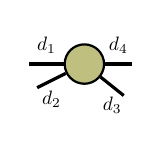
\begin{tikzpicture}[baseline=-0.5ex]
    \tikzset{tensor/.style = {minimum size = 0.5cm,shape = circle,thick,draw=black,inner sep = 0pt}, edge/.style = {thick,line width=.4mm},every loop/.style={}}
    \def\x{6}
    \def\y{0}   \node[tensor,fill=green!50!red!50!white] (T) at (\x+1,\y) {$\Tt$};
    \draw[edge] (T) -- (\x+0.3,0) node [midway,above] {\scalebox{0.7}{\dimcolor{$d_1$}}};
    \draw[edge] (T) -- (\x+1.6,0) node [midway,above] {\scalebox{0.7}{\dimcolor{$d_4$}}};;
    \draw[edge] (T) -- (\x+0.4,-0.3) node [midway, below] {\scalebox{0.7}{\dimcolor{$d_2$}}};
    \draw[edge] (T) -- (\x+1.5,-0.4)node [midway, below] {\scalebox{0.7}{\dimcolor{$d_3$}}};
\end{tikzpicture}
&=
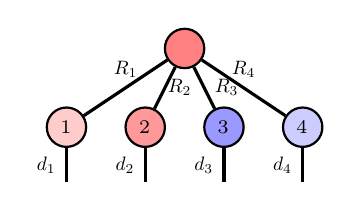
\begin{tikzpicture}[baseline=-0.5ex]
    \tikzset{tensor/.style = {minimum size = 0.5cm,shape = circle,thick,draw=black,inner sep = 0pt}, edge/.style = {thick,line width=.4mm},every loop/.style={}}
    \def\x{6}
    \def\y{0}   
    \node[tensor,fill=red!50!white] (G) at (\x+4.5,\y+1) {$\Gt$};
    \node[tensor,fill=red!20!white] (A_1) at (\x+3,\y){$\Ab_1$};
    \node[tensor,fill=red!40!white] (A_2) at (\x+4,\y){$\Ab_2$};
    \node[tensor, fill=blue!40!white] (A_3) at (\x+5,\y){$\Ab_3$};
    \node[tensor,fill=blue!20!white] (A_4) at (\x+6,\y){$\Ab_4$};
    \draw[edge] (G) -- (A_1) node [midway, above] {\scalebox{0.7}{\dimcolor{$R_1$}}};
    \draw[edge] (G) -- (A_2) node [midway, right=-0.1cm] {\scalebox{0.7}{\dimcolor{$R_2$}}};
    \draw[edge] (G) -- (A_3) node [midway, right=-0.05] {\scalebox{0.7}{\dimcolor{$R_3$}}};
    \draw[edge] (G) -- (A_4) node [midway, above] {\scalebox{0.7}{\dimcolor{$R_4$}}};
    \draw[edge] (A_1) -- (\x+3,\y-0.7) node [midway, left] {\scalebox{0.7}{\dimcolor{$d_1$}}};
    \draw[edge] (A_2) -- (\x+4,\y-0.7) node [midway, left] {\scalebox{0.7}{\dimcolor{$d_2$}}};
    \draw[edge] (A_3) -- (\x+5,\y-0.7) node [midway, left] {\scalebox{0.7}{\dimcolor{$d_3$}}};
    \draw[edge] (A_4) -- (\x+6,\y-0.7) node [midway, left] {\scalebox{0.7}{\dimcolor{$d_4$}}};
\end{tikzpicture}\\
&=
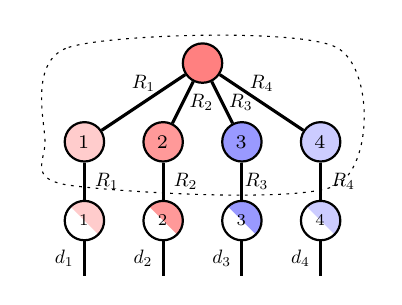
\begin{tikzpicture}[baseline=-0.5ex]
    \tikzset{tensor/.style = {minimum size = 0.5cm,shape = circle,thick,draw=black,inner sep = 0pt}, edge/.style = {thick,line width=.4mm},every loop/.style={}}
    \def\x{6}
    \def\y{0}   
   \node[tensor,fill=red!50!white] (G) at (\x+9,\y+1) {$\Gt$};
    \node[tensor,fill=red!20!white] (R_1) at (\x+7.5,\y){$\Rb_1$};
    \node[tensor,fill=red!40!white] (R_2) at (\x+8.5,\y){$\Rb_2$};
    \node[tensor, fill=blue!40!white] (R_3) at (\x+9.5,\y){$\Rb_3$};
    \node[tensor,fill=blue!20!white] (R_4) at (\x+10.5,\y){$\Rb_4$};
    \node[tensor, path picture={
    \fill[fill=red!20!white](path picture bounding box.south east)
    -- 
    (path picture bounding box.north west) --
    (path picture bounding box.north east) -- cycle;
    }, shift={(\x+7.5,\y-1)}] (Q_1)  {\scalebox{0.85}{$\Qb_1$}};  \node[tensor, path picture={
    \fill[fill=red!40!white](path picture bounding box.south east)
    -- 
    (path picture bounding box.north west) --
    (path picture bounding box.north east) -- cycle;
    }, shift={(\x+8.5,\y-1)}] (Q_2) {\scalebox{0.85}{$\Qb_2$}};
    \node[tensor, path picture={
    \fill[fill=blue!40!white](path picture bounding box.south east)
    -- 
    (path picture bounding box.north west) --
    (path picture bounding box.north east) -- cycle;
    }, shift={(\x+9.5,\y-1)}] (Q_3) {\scalebox{0.85}{$\Qb_3$}};
        \node[tensor, path picture={
    \fill[fill=blue!20!white](path picture bounding box.south east)
    -- 
    (path picture bounding box.north west) --
    (path picture bounding box.north east) -- cycle;
    }, shift={(\x+10.5,\y-1)}] (Q_4) {\scalebox{0.85}{$\Qb_4$}};
    \draw[edge] (G) -- (R_1) node [midway, above] {\scalebox{0.7}{\dimcolor{$R_1$}}};
    \draw[edge] (G) -- (R_2) node [midway, right=-0.05cm] {\scalebox{0.7}{\dimcolor{$R_2$}}};
    \draw[edge] (G) -- (R_3) node [midway, right=-0.05cm] {\scalebox{0.7}{\dimcolor{$R_3$}}};
    \draw[edge] (G) -- (R_4) node [midway, above] {\scalebox{0.7}{\dimcolor{$R_4$}}};
    \draw[edge] (R_1) -- (Q_1) node [midway, right] {\scalebox{0.7}{\dimcolor{$R_1$}}};
    \draw[edge] (R_2) -- (Q_2) node [midway, right] {\scalebox{0.7}{\dimcolor{$R_2$}}};
    \draw[edge] (R_3) -- (Q_3) node [midway, right=-0.1cm] {\scalebox{0.7}{\dimcolor{$R_3$}}};
    \draw[edge] (R_4) -- (Q_4) node [midway, right] {\scalebox{0.7}{\dimcolor{$R_4$}}};
    \draw[edge] (Q_1) -- (\x+7.5,\y-1.7) node [midway, left] {\scalebox{0.7}{\dimcolor{$d_1$}}};
    \draw[edge] (Q_2) -- (\x+8.5,\y-1.7) node [midway, left] {\scalebox{0.7}{\dimcolor{$d_2$}}};
    \draw[edge] (Q_3) -- (\x+9.5,\y-1.7) node [midway, left] {\scalebox{0.7}{\dimcolor{$d_3$}}};
    \draw[edge] (Q_4) -- (\x+10.5,\y-1.7) node [midway, left] {\scalebox{0.7}{\dimcolor{$d_4$}}};
    \draw[dash pattern=on 1pt off 2pt] plot[smooth cycle] coordinates { 
    (\x+7,\y) 
    (\x+7.3, \y+1.2) (\x+10.7,\y+1.2) (\x+10.7, \y-0.55)  (\x+7.3,\y-0.55)};
\end{tikzpicture}
=
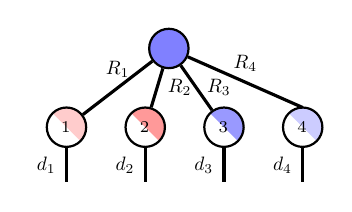
\begin{tikzpicture}[baseline=-0.5ex]
    \tikzset{tensor/.style = {minimum size = 0.5cm,shape = circle,thick,draw=black,inner sep = 0pt}, edge/.style = {thick,line width=.4mm},every loop/.style={}}
    \def\x{6}
    \def\y{0}   
    \node[tensor,fill=blue!50!white] (G) at (\x+13.5,\y+1) {$\Tilde{\Gt}$};
    \node[tensor, path picture={
    \fill[fill=red!20!white](path picture bounding box.south east)
    -- 
    (path picture bounding box.north west) --
    (path picture bounding box.north east) -- cycle;
    }, shift={(\x+12.2,\y)}] (Q_1)  {\scalebox{0.85}{$\Qb_1$}};  \node[tensor, path picture={
    \fill[fill=red!40!white](path picture bounding box.south east)
    -- 
    (path picture bounding box.north west) --
    (path picture bounding box.north east) -- cycle;
    }, shift={(\x+13.2,\y)}] (Q_2) {\scalebox{0.85}{$\Qb_2$}};
    \node[tensor, path picture={
    \fill[fill=blue!40!white](path picture bounding box.south east)
    -- 
    (path picture bounding box.north west) --
    (path picture bounding box.north east) -- cycle;
    }, shift={(\x+14.2,\y)}] (Q_3) {\scalebox{0.85}{$\Qb_3$}};
        \node[tensor, path picture={
    \fill[fill=blue!20!white](path picture bounding box.south east)
    -- 
    (path picture bounding box.north west) --
    (path picture bounding box.north east) -- cycle;
    }, shift={(\x+15.2,\y)}] (Q_4) {\scalebox{0.85}{$\Qb_4$}};
     \draw[edge] (Q_1) -- (\x+12.2,\y-0.7) node [midway, left] {\scalebox{0.7}{\dimcolor{$d_1$}}};
    \draw[edge] (Q_2) -- (\x+13.2,\y-0.7) node [midway, left] {\scalebox{0.7}{\dimcolor{$d_2$}}};
    \draw[edge] (Q_3) -- (\x+14.2,\y-0.7) node [midway, left] {\scalebox{0.7}{\dimcolor{$d_3$}}};
    \draw[edge] (Q_4) -- (\x+15.2,\y-0.7) node [midway, left] {\scalebox{0.7}{\dimcolor{$d_4$}}};
    \draw[edge](G) -- (Q_1)node[midway,above]{\scalebox{0.7}{\dimcolor{$R_1$}}};
    \draw[edge](G) -- (Q_2)node[midway,right]{\scalebox{0.7}{\dimcolor{$R_2$}}};
    \draw[edge](G) -- (Q_3)node[midway,right]{\scalebox{0.7}{\dimcolor{$R_3$}}};
    \draw[edge](G) -- (\x+15.2,\y+0.25)node[midway,above]{\scalebox{0.7}{\dimcolor{$R_4$}}};
\end{tikzpicture}.
\end{align*}
\end{proof}
\item 对于一个 $N$ 阶 $d$ 维张量，在假设 $R_1=\dots=R_N=R$ 之下，其 Tucker 分解的参数个数为 $\bigo(R^N+NdR)$。
\item
本节最后说明，张量的 Tucker 分解的模 $n$ 矩阵化如何用 Kronecker 积来表达。
\begin{proposition}\label{decomp:tucker-kron}
设 $\At\in\RR^{d_1\times d_2\times\dots\times d_N}$。若 $\At=\Gt\ttm{1}\Ub_1\ttm{2}\dots\ttm{N}\Ub_N$，则
$$\At_{(i)}=\Ub_i\Gt_{(i)}\left(\Ub_1\kron\dots\kron\Ub_{(i-1)}\kron\Ub_{(i+1)}\kron\dots\kron\Ub_N\right)^\ts.$$
\begin{proof}
设 $N=3$ 且 $n=1$，则有
\begin{align*}
\At_{(1)}
&=
\left(\begin{tikzpicture}[baseline=\baseline]
    \tikzset{tensor/.style = {minimum size = 0.5cm,shape = circle,thick,draw=black,inner sep = 0pt}, edge/.style  = {thick,line width=.4mm},every loop/.style={}}
    \def\y{0}
    \def\x{0}
    \node[tensor,fill=green!50!red!50!white] (At) at (\x,\y){\scalebox{0.85}{$\At$}};
    \draw[edge] (\x+0.25,\y) -- (\x+0.6,\y)  node [midway,above] {\scalebox{0.7}{\dimcolor{$d_2$}}};
    \draw[edge] (\x-0.25,\y) -- (\x-0.6,\y)  node [midway,above] {\scalebox{0.7}{\dimcolor{$d_1$}}};
    \draw[edge] (\x,\y-0.25) -- (\x,\y-0.7)  node [midway,left] {\scalebox{0.7}{\dimcolor{$d_3$}}};
    \end{tikzpicture}\right)_{(1)}
=
\left(\begin{tikzpicture}[baseline=\baseline]
    \tikzset{tensor/.style = {minimum size = 0.5cm,shape = circle,thick,draw=black,inner sep = 0pt}, edge/.style   = {thick,line width=.4mm},every loop/.style={}}
    \def\y{0}
    \def\x{0}
  \node[tensor,fill=red!50!white] (A1) at (\x,\y){\scalebox{0.85}{$\Ub_1$}};
  \node[tensor,fill=blue!50!white] (A2) at (\x+1,\y){$\Ub_2$};
   \node[tensor,fill=blue!20!white] (A3) at (\x+2,\y){$\Ub_3$};
   \node[tensor,fill=red!60!blue!20!white] (m) at (\x+1,\y+1) {$\Gt$};
    \draw[edge] (A1) -- (m)node [midway,left] {\scalebox{0.7}{\dimcolor{$R_1$}}};
    \draw[edge] (A2) -- (m)node [midway,right=-0.05cm] {\scalebox{0.7}{\dimcolor{$R_2$}}};
    \draw[edge] (A3) -- (m)node [midway,right] {\scalebox{0.7}{\dimcolor{$R_3$}}};
    \draw[edge](A1) -- (\x,\y-0.7)node [midway,left] {\edgelabel{$d_1$}};
    \draw[edge](A2) -- (\x+1,\y-0.7)node [midway,left] {\edgelabel{$d_2$}};
    \draw[edge](A3) -- (\x+2,\y-0.7)node [midway,left] {\edgelabel{$d_3$}};
\end{tikzpicture}\right)_{(1)}\\
&=
\begin{tikzpicture}[baseline=\baseline]
    \tikzset{tensor/.style = {minimum size = 0.5cm,shape = circle,thick,draw=black,inner sep = 0pt}, edge/.style   = {thick,line width=.4mm},every loop/.style={}}
    \def\y{0}
    \def\x{0}
    \node[tensor,fill=green!50!red!50!white] (At) at (\x,\y){\scalebox{0.85}{$\At$}};
    \draw[edge] (\x-0.25,\y) -- (\x-0.6,\y)  node [midway,above] {\scalebox{0.7}{\dimcolor{$d_1$}}};
    \draw[edge] (\x+0.2,\y+0.15) -- (\x+0.5,\y+0.15)-- (\x+0.5,\y+0.05) -- (\x+1,\y+0.05) node [midway,above]
    {\scalebox{0.7}{\dimcolor{$d_2$}}};
    \draw[edge] (\x+0.2,\y-0.15) -- (\x+0.5,\y-0.15)-- (\x+0.5,\y-0.05)-- (\x+1,\y-0.05) node [midway,below]
    {\scalebox{0.7}{\dimcolor{$d_3$}}};
    \end{tikzpicture}
=
\begin{tikzpicture}[baseline=\baseline]
    \tikzset{tensor/.style = {minimum size = 0.5cm,shape = circle,thick,draw=black,inner sep = 0pt}, edge/.style   = {thick,line width=.4mm},every loop/.style={}}
    \def\y{0}
    \def\x{0}
    \node[tensor,fill=red!50!white] (A1) at (\x,\y){\scalebox{0.85}{$\Ub_1$}};
    \node[tensor,fill=blue!50!white] (A2) at (\x+2.7,\y+0.7){$\Ub_2$};
    \node[tensor,fill=blue!20!white] (A3) at (\x+2.7,\y-0.7){$\Ub_3$};
    \node[tensor,fill=red!60!blue!20!white] (m) at (\x+1,\y) {$\Gt$}; 
     \draw[edge] (\x+1.2,\y+0.15) -- (\x+1.5,\y+0.15)-- (\x+1.5,\y+0.05) -- (\x+2,\y+0.05) node [midway,above]
    {\scalebox{0.7}{\dimcolor{$R_2$}}};
    \draw[edge] (\x+1.2,\y-0.15) -- (\x+1.5,\y-0.15)-- (\x+1.5,\y-0.05)-- (\x+2,\y-0.05) node [midway,below]
    {\scalebox{0.7}{\dimcolor{$R_3$}}};
    \draw[edge] (A1) -- (m) node [midway,above] {\scalebox{0.7}{\dimcolor{$R_1$}}};
    \draw[edge] (A1) -- (\x-0.7,\y) node [midway,above] {\scalebox{0.7}{\dimcolor{$d_1$}}};
    \draw[edge](\x+2,\y-0.05) -- (\x+2,\y-0.7) -- (A3);
    \draw[edge](\x+2,\y+0.05) -- (\x+2,\y+0.7) -- (A2);
    \draw[edge] (A2) -- (\x+3.5,\y+0.7) -- (\x+3.5,\y+0.05)-- (\x+4,\y+0.05) node [midway,above]
    {\scalebox{0.7}{\dimcolor{$d_2$}}};
    \draw[edge] (A3) -- (\x+3.5,\y-0.7) -- (\x+3.5,\y-0.05) -- (\x+4,\y-0.05) node [midway,below]
    {\scalebox{0.7}{\dimcolor{$d_3$}}};
    \end{tikzpicture}
=
\Ub_1\Gt_{(1)}(\Ub_2\kron\Ub_3)^\ts.
\end{align*}
\end{proof}
\end{proposition}
\end{enumerate}
\end{remark}
\subsection{张量列~(TT) 分解}\label{sec:tt-decomposition}
张量列~(TT) 分解~\citep{oseledets2010approximation} 是另一种流行的张量分解模型。它将一个 $N$ 阶张量分解为 $N$ 个较小的三阶张量。 
张量 $\St\in\RR^{d_1\times\cdots\times d_N}$ 的秩 $(R_1,\dots,R_{N-1})$ \textit{张量列分解}将其分解为 $N$ 个三阶张量之积\footnote{首尾两个核心可视为矩阵而非三阶张量，因为它们各含一个维数为 1 的模。不过，把它们看作三阶张量能简化一些记法。}，其中 $\Gt_n\in\RR^{R_{n-1}\times d_n\times R_n}$，$n\in [N]$，且 $R_0=R_N=1$：
$$\St_{i_1,\cdots,i_N}= \sum_{r_0=1}^{R_0}\sum_{r_1=1}^{R_1} \cdots \sum_{r_{N-1}=1}^{R_{N-1}}\sum_{r_N=1}^{R_N} \prod_{n=1}^N\Gt_n(r_{n-1},i_n,r_n) := \TT(({\Gt_n})_{n=1}^N),$$ 
对所有 $i_1\in[d_1],\cdots,i_N\in[d_N]$ 成立。  
$\St$ 的\emph{TT 秩}是满足如下条件的最小
$(R_1,R_2,\dots,R_{N-1})$：$\St$ 存在精确的秩 $(R_1,R_2,\dots,R_{N-1})$ 的 TT 分解 $\St=\TT(({\Gt_n})_{n=1}^N)$。
与 CP 分解和 Tucker 分解类似，这里的秩可视为控制 TT 分解表达能力的超参数。也就是说，只要秩足够大，TT 分解就能表示任意张量。下面的张量网络展示了四阶张量的秩 $(R_1,R_2,R_3)$ TT 分解：

$$
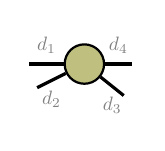
\begin{tikzpicture}[baseline=-0.5ex]
    \tikzset{tensor/.style = {minimum size = 0.5cm,shape = circle,thick,draw=black,inner sep = 0pt}, edge/.style = {thick,line width=.4mm},every loop/.style={}}
    \def\x{6}
    \def\y{0}
     \node[tensor,fill=green!50!red!50!white] (B) at (\x+1,\y) {$\St$};
    \draw[edge] (B) -- (\x+0.3,0) node [midway,above] {\scalebox{0.7}{\textcolor{gray}{$d_1$}}};
    \draw[edge] (B) -- (\x+1.6,0) node [midway,above] {\scalebox{0.7}{\textcolor{gray}{$d_4$}}};;
    \draw[edge] (B) -- (\x+0.4,-0.3) node [midway, below] {\scalebox{0.7}{\textcolor{gray}{$d_2$}}};;
    \draw[edge] (B) -- (\x+1.5,-0.4)node [midway, below] {\scalebox{0.7}{\textcolor{gray}{$d_3$}}};;
\end{tikzpicture}=
\begin{tikzpicture}[baseline=\baseline]
    \tikzset{tensor/.style = {minimum size = 0.5cm,shape = circle,thick,draw=black,inner sep = 0pt}, edge/.style   = {thick,line width=.4mm},every loop/.style={}}
    \def\y{0}
    \def\x{0}
  \node[tensor,fill=red!30!white] (D) at (\x-1,\y){$\Gt_1$};
  \node[tensor,fill=red!50!white] (A) at (\x,\y){\scalebox{0.85}{$\Gt_2$}};
  \node[tensor,fill=blue!50!white] (B) at (\x+1,\y){$\Gt_3$};
   \node[tensor,fill=blue!20!white] (C) at (\x+2,\y){$\Gt_4$};
    \draw[edge](A) -- (\x,\y-0.7)node [midway,left] {\edgelabel{$d_2$}};
    \draw[edge](B) -- (\x+1,\y-0.7)node [midway,left] {\edgelabel{$d_3$}};
    \draw[edge](C) -- (\x+2,\y-0.7)node [midway,left] {\edgelabel{$d_4$}};
     \draw[edge](D) -- (\x-1,\y-0.7)node [midway,left] {\edgelabel{$d_1$}};
    \draw[edge](D) -- (A) node [midway,above] {\edgelabel{$R_1$}};
    \draw[edge](A) -- (B) node [midway,above] {\edgelabel{$R_2$}};
    \draw[edge](B) -- (C) node [midway,above] {\edgelabel{$R_3$}};
\end{tikzpicture}.
$$
TT 分解最早在量子物理与凝聚态物理社区中以 \emph{矩阵乘积态}（Matrix Product States, MPS）之名提出。在这一语境下，内部边的维数被称为 \textit{键维数}，自由腿则称为 \textit{物理维数}。
接下来我们说明如何在多项式时间内，利用逐次奇异值分解（SVD）计算张量 $\St\in\RR^{d_1\times\dots\times d_N}$ 的精确 TT 分解。该算法被称为 TT-SVD 算法~\citep{oseledets2010approximation}，但更早由量子物理社区引入，并被称作 \textit{逐次 Schmidt 分解}~\citep{vidal2004efficient,mcculloch2007density}。
在给出 TT-SVD 算法之前，先介绍三阶张量的左正交与右正交概念。
\begin{definition}\label{def:left-right-ortho}若 $(\At_n)_{(3)}^\ts(\At_n)_{(3)}=\Ib_{R_n}$，则称 $n\in[N]$ 对应的核心张量 $\At_n\in\RR^{R_{n-1}\times d_n\times R_n}$ 左正交；若 $(\At_n)_{(1)}(\At_n)_{(1)}^\ts=\Ib_{R_{n-1}}$，则称其右正交。这可以用张量网络
图示如下：
\begin{align*}
\begin{tikzpicture}[baseline=\baseline]
    \tikzset{tensor/.style = {minimum size = 0.5cm,shape = circle,thick,draw=black,inner sep = 0pt}, edge/.style = {thick,line width=.4mm},every loop/.style={}}
    \def\y{0}
    \def\x{0}
    \node[tensor, path picture={
    \fill[fill=red!30!white](path picture bounding box.south east)
        -- 
    (path picture bounding box.north west) --
    (path picture bounding box.north east) -- cycle;
    }, shift={(\x,\y)}] (A) {\scalebox{0.85}{$\At_n$}};
    \draw[edge](A) -- (\x,\y-0.7)node [midway,left] {\scalebox{0.7}{\dimcolor{$d_n$}}};
    \draw[edge](A) -- (\x-0.85,\y)node [midway,above] {\scalebox{0.7}{\dimcolor{$R_{n-1}$}}};
    \draw[edge](A) -- (\x+0.85,\y)node [midway,above] {\scalebox{0.7}{\dimcolor{$R_n$}}};
\end{tikzpicture}\ \  \text{is left-orthogonal}
\iff
\begin{tikzpicture}[baseline=\baseline]
    \tikzset{tensor/.style = {minimum size = 0.5cm,shape = circle,thick,draw=black,inner sep = 0pt}, edge/.style = {thick,line width=.4mm},every loop/.style={}}
    \def\y{0}
    \def\x{0}
    \node[tensor, path picture={
    \fill[fill=red!30!white](path picture bounding box.south west)
        -- 
    (path picture bounding box.north east) --
    (path picture bounding box.north west) -- cycle;
    }, shift={(\x,\y)}] (A1) {\scalebox{0.85}{$\At_n$}};
    \node[tensor, path picture={
    \fill[fill=red!30!white](path picture bounding box.south east)
        -- 
    (path picture bounding box.north west) --
    (path picture bounding box.north east) -- cycle;
    }, shift={(\x+1,\y)}] (A2) {\scalebox{0.85}{$\At_n$}};
    \draw[edge](A1)--(A2)node [midway,above] {\scalebox{0.7}{\dimcolor{$R_{n-1}$}}};
    \draw[edge](\x+0.23,\y-0.1) -- (\x+0.77,\y-0.1) node [midway,below] {\scalebox{0.7}{\dimcolor{$d_n$}}};
    \draw[edge](A1) -- (\x-0.85,\y)node [midway,above] {\scalebox{0.7}{\dimcolor{$R_{n}$}}};
    \draw[edge](A2) -- (\x+1.85,\y)node [midway,above] {\scalebox{0.7}{\dimcolor{$R_{n}$}}};
\end{tikzpicture}
=
\begin{tikzpicture}[baseline=\baseline]
    \tikzset{tensor/.style = {minimum size = 0.5cm,shape = circle,thick,draw=black,inner sep = 0pt}, edge/.style = {thick,line width=.4mm},every loop/.style={}}
    \def\y{0}
    \def\x{0}
    \draw[edge](\x,\y) -- (\x+1.5,\y)node [midway,above] {\scalebox{0.7}{\dimcolor{$R_n$}}};
\end{tikzpicture}=\Ib_{R_n},
\end{align*}
类似地，
\begin{align*}
\begin{tikzpicture}[baseline=\baseline]
    \tikzset{tensor/.style = {minimum size = 0.5cm,shape = circle,thick,draw=black,inner sep = 0pt}, edge/.style = {thick,line width=.4mm},every loop/.style={}}
    \def\y{0}
    \def\x{0}
    \node[tensor, path picture={
    \fill[fill=blue!30!white](path picture bounding box.south west)
        -- 
    (path picture bounding box.north east) --
    (path picture bounding box.north west) -- cycle;
    }, shift={(\x,\y)}] (A) {\scalebox{0.85}{$\At_n$}};
    \draw[edge](A) -- (\x,\y-0.7)node [midway,left] {\scalebox{0.7}{\dimcolor{$d_n$}}};
    \draw[edge](A) -- (\x-0.85,\y)node [midway,above] {\scalebox{0.7}{\dimcolor{$R_{n-1}$}}};
    \draw[edge](A) -- (\x+0.85,\y)node [midway,above] {\scalebox{0.7}{\dimcolor{$R_n$}}};
\end{tikzpicture}\ \  \text{is right-orthogonal}
\iff
\begin{tikzpicture}[baseline=\baseline]
    \tikzset{tensor/.style = {minimum size = 0.5cm,shape = circle,thick,draw=black,inner sep = 0pt}, edge/.style = {thick,line width=.4mm},every loop/.style={}}
    \def\y{0}
    \def\x{0}
    \node[tensor, path picture={
    \fill[fill=blue!30!white](path picture bounding box.south west)
        -- 
    (path picture bounding box.north east) --
    (path picture bounding box.north west) -- cycle;
    }, shift={(\x,\y)}] (A1) {\scalebox{0.85}{$\At_n$}};
    \node[tensor, path picture={
    \fill[fill=blue!30!white](path picture bounding box.south east)
        -- 
    (path picture bounding box.north west) --
    (path picture bounding box.north east) -- cycle;
    }, shift={(\x+1,\y)}] (A2) {\scalebox{0.85}{$\At_n$}};
    \draw[edge](A1)--(A2)node [midway,above] {\scalebox{0.7}{\dimcolor{$R_{n}$}}};
    \draw[edge](A1) -- (\x-0.85,\y)node [midway,above] {\scalebox{0.7}{\dimcolor{$R_{n-1}$}}};
    \draw[edge](A2) -- (\x+1.85,\y)node [midway,above] {\scalebox{0.7}{\dimcolor{$R_{n-1}$}}};
    \draw[edge](\x+0.23,\y-0.1) -- (\x+0.77,\y-0.1) node [midway,below] {\scalebox{0.7}{\dimcolor{$d_n$}}};
\end{tikzpicture}
=
\begin{tikzpicture}[baseline=\baseline]
    \tikzset{tensor/.style = {minimum size = 0.5cm,shape = circle,thick,draw=black,inner sep = 0pt}, edge/.style = {thick,line width=.4mm},every loop/.style={}}
    \def\y{0}
    \def\x{0}
    \draw[edge](\x,\y) -- (\x+1.5,\y)node [midway,above] {\scalebox{0.7}{\dimcolor{$R_{n-1}$}}};
\end{tikzpicture}=\Ib_{R_{n-1}}.
\end{align*}
\end{definition}
下面的定理说明任意张量都存在最小的张量列（TT）分解，其证明是构造性的，给出了 TT-SVD 算法的流程。
\begin{theorem}(\textbf{计算（正交）张量列分解。})\label{thm:tt-decomposition}
对任意 $\St\in\RR^{d_1\times\dots\times d_N}$，设 $\St_{([n])}\in\RR^{d_1\dots d_n\times d_{n+1}\dots d_N}$ 为把 $\St$ 的前 $n$  个模映射到 $\St_{[n]}$ 的行上所得到的矩阵化。则 $\St$ 的 TT 秩 $(R_1,\cdots,R_{N-1})$ 由
    下式给出
    $R_n = \rank~(\St_{([n])})$ 对所有 $n\in[N-1]$ 成立。
\end{theorem}
\begin{proof}
    设 $R_n = \rank~(\St_{([n])})$。我们先说明如何用逐次 QR 分解构造出 $\St\in\RR^{d_1\times\cdots\times d_N}$ 的一个秩为 $(R_1,R_2,\cdots,R_{N-1})$ 的 TT 分解。为简单起见，只考虑 $N=4$ 的情形，但上述论证很容易推广。

我们先对 $\ten S$ 的第一模矩阵化做 QR 分解，该矩阵化的秩为 $R_1$：
\begin{align*}
    \begin{tikzpicture}[baseline=\baseline]
    \tikzset{tensor/.style = {minimum size = 0.5cm,shape = circle,thick,draw=black,inner sep = 0pt}, edge/.style = {thick,line width=.4mm},every loop/.style={}}
    \def\y{0}
    \def\x{0}
    \node[tensor,fill=green!50!red!50!white] (A) at (\x-5.5,\y){\scalebox{0.85}{$\St$}};
    \draw[edge] (A) -- (\x-5.5,\y+0.75) node [midway,left]
    {\scalebox{0.7}{\dimcolor{$d_1$}}};
    \draw[edge] (A) -- (\x-5.5,\y-0.75) node [midway,left]
    {\scalebox{0.7}{\dimcolor{$d_3$}}};
    \draw[edge] (\x-5.75,\y+0.05) -- (\x-6.2,\y-0.3) node [midway,above]
    {\scalebox{0.7}{\dimcolor{$d_2$}}};
    \draw[edge] (\x-5.25,\y+0.05) -- (\x-4.7,\y-0.3) node [midway,above]
    {\scalebox{0.7}{\dimcolor{$d_4$}}};
    \node[draw=none] at (\x-3,\y){$\underrightarrow{\text{mode-1 matricization}}$};
    %
    %
    %
    %
    \node[tensor,fill=green!50!red!50!white] (A) at (\x-0.5,\y){\scalebox{0.85}{$\St$}};
    \draw[edge] (\x-0.35,\y+0.2) -- (\x,\y+0.2) --(\x,\y+0.1) -- (\x
    +0.35,\y+0.1) node [midway,above]
    {\scalebox{0.7}{\dimcolor{$d_2$}}};
    \draw[edge] (\x-0.35,\y-0.2) -- (\x,\y-0.2) -- (\x,\y-0.1) -- (\x+0.35,\y-0.1) node [midway,below]
    {\scalebox{0.7}{\dimcolor{$d_4$}}};
     \draw[edge] (A) -- (\x+0.35,\y)node [right]
    {\scalebox{0.7}{\dimcolor{$d_3$}}};
     \draw[edge] (A) -- (\x-1.25,\y) node [midway,above]
    {\scalebox{0.7}{\dimcolor{$d_1$}}};
    \node[draw=none] at (\x+1.25,\y){$\underrightarrow{\text{QR}}$};
    %
    %
    %
    \node[tensor, path picture={
    \fill[fill=blue!50!white](path picture bounding box.south east)
        -- 
    (path picture bounding box.north west) --
    (path picture bounding box.north east) -- cycle;
    }, shift={(\x+2,\y)}] (Q_1) {\scalebox{0.8}{$\Qb_1$}};
    \node[tensor,fill=red!50!white] (R_1) at (\x+3,\y){\scalebox{0.85}{$\Rb_1$}};
    \draw[edge] (Q_1) -- (\x+2,\y-0.75) node [midway,left]
    {\scalebox{0.7}{\dimcolor{$d_1$}}};
    \draw[edge] (Q_1) -- (R_1) node [midway,above]
    {\scalebox{0.7}{\dimcolor{$R_1$}}};
    \draw[edge] (\x+3.15,\y+0.2) -- (\x+3.5,\y+0.2) --(\x+3.5,\y+0.1) -- (\x+4,\y+0.1) node [midway,above]
    {\scalebox{0.7}{\dimcolor{$d_2$}}};
    \draw[edge] (\x+3.15,\y-0.2) -- (\x+3.5,\y-0.2) -- (\x+3.5,\y-0.1) -- (\x+4,\y-0.1) node [midway,below]
    {\scalebox{0.7}{\dimcolor{$d_4$}}};
    \draw[edge] (R_1) -- (\x+4,\y) node [right]
    {\scalebox{0.7}{\dimcolor{$d_3$}}};
    \node[draw=none] at (\x+6.5,\y){\text{Keep $\Qb_1$, resume with $\Rb_1$.}};
    \end{tikzpicture}
\end{align*}
然后，我们对上一步得到的 $\mat R_1$ 再做一次 QR 分解：
\begin{align*}
    \begin{tikzpicture}[baseline=\baseline]
    \tikzset{tensor/.style = {minimum size = 0.5cm,shape = circle,thick,draw=black,inner sep = 0pt}, edge/.style = {thick,line width=.4mm},every loop/.style={}}
    \def\y{0}
    \def\x{0}
    \node[tensor,fill=red!50!white] (R_1) at (\x-5.5,\y){\scalebox{0.85}{$\Rb_1$}};
    \draw[edge] (R_1) -- (\x-6.5,\y) node [midway,above]
    {\scalebox{0.7}{\dimcolor{$R_1$}}};
    \draw[edge] (\x-5.35,\y+0.2) -- (\x-5,\y+0.2) -- (\x-5,\y+0.1) -- (\x-4.5,\y+0.1) node [midway,above]
    {\scalebox{0.7}{\dimcolor{$d_2$}}};
    \draw[edge] (\x-5.35,\y-0.2) -- (\x-5,\y-0.2) -- (\x-5,\y-0.1) -- (\x-4.5,\y-0.1) node [midway,below]
    {\scalebox{0.7}{\dimcolor{$d_4$}}};
    \draw[edge] (R_1) -- (\x-4.5,\y) node [right]
    {\scalebox{0.7}{\dimcolor{$d_3$}}};
    \node[draw=none] at (\x-3.25,\y){$\underrightarrow{\text{reshape}}$};
    \node[tensor,fill=red!50!white] (R_1) at (\x-1.25,\y){\scalebox{0.85}{$\Rb_1$}};
    \draw[edge] (R_1) -- (\x-2.25,\y) node [midway,above]
    {\scalebox{0.7}{\dimcolor{$R_1$}}};
    \draw[edge] (\x-1.5,\y-0.1) -- (\x-2.25,\y-0.1) node [midway,below]
    {\scalebox{0.7}{\dimcolor{$d_2$}}};
    \draw[edge] (\x-1.1,\y-0.2) -- (\x-0.7,\y-0.2) -- (\x-0.7,\y-0.1) -- (\x-0.35,\y-0.1) node [midway,below]
    {\scalebox{0.7}{\dimcolor{$d_4$}}};
    \draw[edge] (R_1) -- (\x-0.35,\y) node [right]
    {\scalebox{0.7}{\dimcolor{$d_3$}}};
    \node[draw=none] at (\x+0.5,\y){$\underrightarrow{\text{QR}}$};
    \node[tensor, path picture={
    \fill[fill=blue!30!white](path picture bounding box.south east)
        -- 
    (path picture bounding box.north west) --
    (path picture bounding box.north east) -- cycle;
    }, shift={(\x+1.5,\y)}] (Q_2) {\scalebox{0.8}{$\Qb_2$}};
    \node[tensor,fill=red!50!white] (R_2) at (\x+2.5,\y){\scalebox{0.85}{$\Rb_2$}};
    \draw[edge] (Q_2) -- (\x+1.5,\y-0.75) node [midway,left=0.1cm]
    {\scalebox{0.7}{\dimcolor{$d_2$}}};
    \draw[edge] (\x+1.38,\y-0.22) -- (\x+1.38,\y-0.75) node [midway,right=0.1cm]
    {\scalebox{0.7}{\dimcolor{$R_1$}}};
    \draw[edge] (Q_2) -- (R_2) node [midway,above]
    {\scalebox{0.7}{\dimcolor{$R_2$}}};
    \draw[edge] (\x+2.65,\y-0.2) -- (\x+3,\y-0.2) -- (\x+3,\y-0.1) -- (\x+3.45,\y-0.1) node [midway,below]
    {\scalebox{0.7}{\dimcolor{$d_4$}}};
    \draw[edge] (R_2) -- (\x+3.45,\y) node [right]
    {\scalebox{0.7}{\dimcolor{$d_3$}}};
    \node[draw=none] at (\x+6,\y){\text{Keep $\Qb_2$}, resume with $\Rb_2$.};
    \end{tikzpicture}
\end{align*}\\
要使这一精确 QR 分解的秩为 $R_2$，我们首先需要证明：
将 $\Rb_1$ 重排成 $R_1d_2 \times d_3d_4$ 矩阵后，其秩至多为 $R_2$。注意到，由于 $\rank(\St_{([2])}) = R_2$，
存在 $\Ab \in \RR^{d_1 d_2 \times R_2}$ 与
$\Bb \in \RR^{R_2 \times d_3 d_4}$ 使得 $\St_{([2])} = \Ab\Bb$，即
$$
\begin{tikzpicture}[baseline=\baseline]
\tikzset{
  tensor/.style = {minimum size = 0.5cm,shape = circle,thick,draw=black,inner sep = 0pt},
  edge/.style   = {thick,line width=.4mm},
  every loop/.style={}
}
\def\y{0}
\def\x{0}
\node[tensor,fill=green!50!red!50!white] (A) at (\x-5.5,\y){\scalebox{0.85}{$\St$}};
\draw[edge] (A) -- (\x-5.5,\y+0.75) node [midway,left]
{\scalebox{0.7}{\dimcolor{$d_1$}}};
\draw[edge] (A) -- (\x-5.5,\y-0.75) node [midway,left]
{\scalebox{0.7}{\dimcolor{$d_3$}}};
\draw[edge] (\x-5.75,\y+0.05) -- (\x-6.2,\y-0.3) node [midway,above]
{\scalebox{0.7}{\dimcolor{$d_2$}}};
\draw[edge] (\x-5.25,\y+0.05) -- (\x-4.7,\y-0.3) node [midway,above]
{\scalebox{0.7}{\dimcolor{$d_4$}}};
\end{tikzpicture}
\ \ \ \underrightarrow{\text{reshape}}\ \ \ 
\begin{tikzpicture}[baseline=\baseline]
\tikzset{
  tensor/.style = {minimum size = 0.5cm,shape = circle,thick,draw=black,inner sep = 0pt},
  edge/.style   = {thick,line width=.4mm},
  every loop/.style={}
}
\def\y{0}
\def\x{0}
\node[tensor,fill=green!50!red!50!white] (A) at (\x+0.5,\y){\scalebox{0.85}{$\St$}};
\draw[edge] (\x+0.25,\y+0.1) -- (\x-0.35,\y+0.1) node [midway,above]
{\scalebox{0.7}{\dimcolor{$d_1$}}};
\draw[edge] (\x+0.75,\y-0.1) -- (\x+1.35,\y-0.1) node [midway,below]
{\scalebox{0.7}{\dimcolor{$d_4$}}};
\draw[edge] (A) -- (\x+1.35,\y) node [midway,above]
{\scalebox{0.7}{\dimcolor{$d_3$}}};
\draw[edge] (A) -- (\x-0.35,\y) node [midway,below]
{\scalebox{0.7}{\dimcolor{$d_2$}}};
\end{tikzpicture}
\ \ \ =\ \ \ 
\begin{tikzpicture}[baseline=\baseline]
\tikzset{
  tensor/.style = {minimum size = 0.5cm,shape = circle,thick,draw=black,inner sep = 0pt},
  edge/.style   = {thick,line width=.4mm},
  every loop/.style={}
}
\def\y{-0.05}
\def\x{0}
\node[tensor,fill=blue!50!red!50!white] (B) at (\x+6.5,\y){\scalebox{0.85}{$\Ab$}};
\node[tensor,fill=blue!50!red!20!white] (C) at (\x+7.5,\y){\scalebox{0.85}{$\Bb$}};
\draw[edge] (B) -- (C) node [midway,above]
{\scalebox{0.7}{\dimcolor{$R_2$}}};
\draw[edge] (B) -- (\x+5.5,\y) node [midway,below]
{\scalebox{0.7}{\dimcolor{$d_2$}}};
\draw[edge] (\x+6.25,\y+0.1) -- (\x+5.5,\y+0.1) node [midway,above]
{\scalebox{0.7}{\dimcolor{$d_1$}}};
\draw[edge] (C) -- (\x+8.5,\y) node [midway,above]
{\scalebox{0.7}{\dimcolor{$d_3$}}};
\draw[edge] (\x+7.75,\y-0.1) -- (\x+8.5,\y-0.1) node [midway,below]
{\scalebox{0.7}{\dimcolor{$d_4$}}};
\end{tikzpicture}.
$$

将 $\Qb_1$ 与第一模矩阵化 $\Sb_{(1)}$ 收缩，并利用上面的分解式，可得
\begin{align}\label{eq:tt-qr-fac}
    \begin{tikzpicture}[baseline=\baseline]
    \tikzset{tensor/.style = {minimum size = 0.5cm,shape = circle,thick,draw=black,inner sep = 0pt}, edge/.style = {thick,line width=.4mm},every loop/.style={}}
    \def\y{0}
    \def\x{0}
    \node[tensor, path picture={
    \fill[fill=blue!50!white](path picture bounding box.south west)
        -- 
    (path picture bounding box.north east) --
    (path picture bounding box.north west) -- cycle;
    }, shift={(\x-5.5,\y)}] (Q_1) {\scalebox{0.8}{$\Qb_1$}};
    \node[tensor,fill=green!50!red!50!white] (S) at (\x-4.5,\y){\scalebox{0.85}{$\St$}};
    \draw[edge](Q_1) -- (S)node [midway,above]
    {\scalebox{0.7}{\dimcolor{$d_1$}}};
    \draw[edge](Q_1) -- (\x-6.5,\y)node [midway,above]
    {\scalebox{0.7}{\dimcolor{$R_1$}}};
    \draw[edge](S) -- (\x-3.5,\y)node [right]
    {\scalebox{0.7}{\dimcolor{$d_3$}}};
    \draw[edge](\x-4.25,\y-0.1) -- (\x-3.5,\y-0.1)node [midway,below]
    {\scalebox{0.7}{\dimcolor{$d_4$}}};
    \draw[edge](\x-4.25,\y+0.1) -- (\x-3.5,\y+0.1)node [midway,above]
    {\scalebox{0.7}{\dimcolor{$d_2$}}};
\end{tikzpicture}
=
\begin{tikzpicture}[baseline=\baseline]
    \tikzset{tensor/.style = {minimum size = 0.5cm,shape = circle,thick,draw=black,inner sep = 0pt}, edge/.style = {thick,line width=.4mm},every loop/.style={}}
    \def\y{0}
    \def\x{0}
    \node[tensor, path picture={
    \fill[fill=blue!50!white](path picture bounding box.south west)
        -- 
    (path picture bounding box.north east) --
    (path picture bounding box.north west) -- cycle;
    }, shift={(\x-5.5,\y)}] (Q_1) {\scalebox{0.8}{$\Qb_1$}};
    \node[tensor,fill=green!50!red!50!white] (S) at (\x-4.5,\y){\scalebox{0.85}{$\St$}};
    \draw[edge](Q_1) -- (S)node [midway,above]
    {\scalebox{0.7}{\dimcolor{$d_1$}}};
    \draw[edge](Q_1) -- (\x-6.5,\y)node [midway,above]
    {\scalebox{0.7}{\dimcolor{$R_1$}}};
    \draw[edge](S) -- (\x-3.5,\y)node [right]
    {\scalebox{0.7}{\dimcolor{$d_3$}}};
    \draw[edge](\x-4.25,\y-0.1) -- (\x-3.5,\y-0.1)node [midway,below]
    {\scalebox{0.7}{\dimcolor{$d_4$}}};
    \draw[edge](\x-4.5,\y-0.25) -- (\x-4.5,\y-0.45) -- (\x-5.8,\y-0.45)node [midway,below]
    {\scalebox{0.7}{\dimcolor{$d_2$}}} -- (\x-5.8,\y-0.1)-- (\x-6.5,\y-0.1);
\end{tikzpicture}
=
\begin{tikzpicture}
    [baseline=\baseline]
    \tikzset{tensor/.style = {minimum size = 0.5cm,shape = circle,thick,draw=black,inner sep = 0pt}, edge/.style = {thick,line width=.4mm},every loop/.style={}}
    \def\y{0}
    \def\x{0}    
    \node[tensor, path picture={
    \fill[fill=blue!50!white](path picture bounding box.south west)
        -- 
    (path picture bounding box.north east) --
    (path picture bounding box.north west) -- cycle;
    }, shift={(\x,\y)}] (Q_1) {\scalebox{0.8}{$\Qb_1$}};
    \node[tensor,fill=blue!50!red!50!white] (A) at (\x+1,\y){\scalebox{0.85}{$\Ab$}};
    \node[tensor,fill=blue!50!red!20!white] (B) at (\x+2.5,\y){\scalebox{0.85}{$\Bb$}};
    \draw[edge] (A) -- (B) node [midway,above]
    {\scalebox{0.7}{\dimcolor{$R_2$}}};
    \draw[edge] (Q_1) -- (A) node [midway,above]
    {\scalebox{0.7}{\dimcolor{$d_1$}}};
    \draw[edge] (Q_1) -- (\x-1,\y) node [midway,above]
    {\scalebox{0.7}{\dimcolor{$R_1$}}};
    \draw[edge] (\x+2.74,\y-0.1) -- (\x+3.5,\y-0.1) node [midway,below]
    {\scalebox{0.7}{\dimcolor{$d_4$}}};
    \draw[edge] (B) -- (\x+3.5,\y) node [midway,above]
    {\scalebox{0.7}{\dimcolor{$d_3$}}};
 \draw[edge](\x+1,\y-0.25) -- (\x+1,\y-0.45) -- (\x-0.3,\y-0.45)node [midway,below]
    {\scalebox{0.7}{\dimcolor{$d_2$}}} -- (\x-0.3,\y-0.1)-- (\x-1,\y-0.1);
\end{tikzpicture}.
\end{align}
此外，由于 $\Qb_1$ 正交且来自 $\Sb_{(1)}$ 的 QR 分解，故 $\Qb_1\Sb_{(1)}$ 等于 $\Rb_1$，于是：
\begin{align}\label{eq:tt-equal-r1}
    \begin{tikzpicture}[baseline=\baseline]
    \tikzset{tensor/.style = {minimum size = 0.5cm,shape = circle,thick,draw=black,inner sep = 0pt}, edge/.style = {thick,line width=.4mm},every loop/.style={}}
    \def\y{0}
    \def\x{0}
    \node[tensor, path picture={
    \fill[fill=blue!50!white](path picture bounding box.south west)
        -- 
    (path picture bounding box.north east) --
    (path picture bounding box.north west) -- cycle;
    }, shift={(\x-5.5,\y)}] (Q_1) {\scalebox{0.8}{$\Qb_1$}};
    \node[tensor,fill=green!50!red!50!white] (S) at (\x-4.5,\y){\scalebox{0.85}{$\St$}};
    \draw[edge](Q_1) -- (S)node [midway,above]
    {\scalebox{0.7}{\dimcolor{$d_1$}}};
    \draw[edge](Q_1) -- (\x-6.5,\y)node [midway,above]
    {\scalebox{0.7}{\dimcolor{$R_1$}}};
    \draw[edge](S) -- (\x-3.5,\y)node [right]
    {\scalebox{0.7}{\dimcolor{$d_3$}}};
    \draw[edge](\x-4.25,\y-0.1) -- (\x-3.5,\y-0.1)node [midway,below]
    {\scalebox{0.7}{\dimcolor{$d_4$}}};
    \draw[edge](\x-4.5,\y-0.25) -- (\x-4.5,\y-0.45) -- (\x-5.8,\y-0.45)node [midway,below]
    {\scalebox{0.7}{\dimcolor{$d_2$}}} -- (\x-5.8,\y-0.1)-- (\x-6.5,\y-0.1);
   \def\x{-3}
     \node[draw=none] at (\x+0.2,\y){$=$};
   \node[tensor, path picture={
    \fill[fill=blue!50!white](path picture bounding box.south west)
        -- 
    (path picture bounding box.north east) --
    (path picture bounding box.north west) -- cycle;
    }, shift={(\x+1.5,\y)}] (Q_1) {\scalebox{0.8}{$\Qb_1$}};
    \node[tensor, path picture={
    \fill[fill=blue!50!white](path picture bounding box.south east)
        -- 
    (path picture bounding box.north west) --
    (path picture bounding box.north east) -- cycle;
    }, shift={(\x+2.5,\y)}] (Q_1t) {\scalebox{0.8}{$\Qb_1$}};
    \node[tensor,fill=red!50!white] (R_1) at (\x+3.5,\y){\scalebox{0.85}{$\Rb_1$}};
    \draw[edge](Q_1) -- (\x+0.5,\y) node [midway,above]
    {\scalebox{0.7}{\dimcolor{$R_1$}}};
    \draw[edge](Q_1) -- (Q_1t) node [midway,above]
    {\scalebox{0.7}{\dimcolor{$d_1$}}};
 \draw[edge](\x+3.5,\y-0.25) -- (\x+3.5,\y-0.45) -- (\x+1.1,\y-0.45)node [midway,below]
    {\scalebox{0.7}{\dimcolor{$d_2$}}} -- (\x+1.1,\y-0.1)-- (\x+0.5,\y-0.1);
    \draw[edge] (\x+3.65,\y-0.2) -- (\x+4,\y-0.2) -- (\x+4,\y-0.1) -- (\x+4.5,\y-0.1) node [midway,below]
    {\scalebox{0.7}{\dimcolor{$d_4$}}};
    \draw[edge] (R_1) -- (\x+4.5,\y) node [right]
    {\scalebox{0.7}{\dimcolor{$d_3$}}};
    \draw[edge](Q_1t) -- (R_1) node [midway,above]
    {\scalebox{0.7}{\dimcolor{$R_1$}}};
    \node[draw=none] at (\x+5.25,\y){$=$};
    \node[tensor,fill=red!50!white] (R_1) at (\x+6.5,\y){\scalebox{0.85}{$\Rb_1$}};
    \draw[edge] (\x+6.28,\y-0.1) -- (\x+5.5, \y-0.1) node [midway,below]
    {\scalebox{0.7}{\dimcolor{$d_2$}}};
    \draw[edge] (\x+6.65,\y-0.2) -- (\x+7,\y-0.2) -- (\x+7,\y-0.1) -- (\x+7.5,\y-0.1) node [midway,below]
    {\scalebox{0.7}{\dimcolor{$d_4$}}};
    \draw[edge] (R_1) -- (\x+7.5,\y) node [midway,above]
    {\scalebox{0.7}{\dimcolor{$d_3$}}};
    \draw[edge] (R_1) -- (\x+5.5,\y) node [midway, above]
    {\scalebox{0.7}{\dimcolor{$R_1$}}};
\end{tikzpicture}.
\end{align}
结合恒等式~\eqref{eq:tt-qr-fac} 与~\eqref{eq:tt-equal-r1}，可得
$$
\begin{tikzpicture}[baseline=\baseline]
    \tikzset{tensor/.style = {minimum size = 0.5cm,shape = circle,thick,draw=black,inner sep = 0pt}, edge/.style = {thick,line width=.4mm},every loop/.style={}}
    \def\x{-6}
    \def\y{0}
    \node[tensor,fill=red!50!white] (R_1) at (\x+6.5,\y){\scalebox{0.85}{$\Rb_1$}};
    \draw[edge] (\x+6.28,\y-0.1) -- (\x+5.5, \y-0.1) node [midway,below]
    {\scalebox{0.7}{\dimcolor{$d_2$}}};
    \draw[edge] (\x+6.65,\y-0.2) -- (\x+7,\y-0.2) -- (\x+7,\y-0.1) -- (\x+7.5,\y-0.1) node [midway,below]
    {\scalebox{0.7}{\dimcolor{$d_4$}}};
    \draw[edge] (R_1) -- (\x+7.5,\y) node [midway,above]
    {\scalebox{0.7}{\dimcolor{$d_3$}}};
    \draw[edge] (R_1) -- (\x+5.5,\y) node [midway, above]
    {\scalebox{0.7}{\dimcolor{$R_1$}}};
\end{tikzpicture}
=
\begin{tikzpicture}
    [baseline=\baseline]
    \tikzset{tensor/.style = {minimum size = 0.5cm,shape = circle,thick,draw=black,inner sep = 0pt}, edge/.style = {thick,line width=.4mm},every loop/.style={}}
    \def\y{0}
    \def\x{0}    
    \node[tensor, path picture={
    \fill[fill=blue!50!white](path picture bounding box.south west)
        -- 
    (path picture bounding box.north east) --
    (path picture bounding box.north west) -- cycle;
    }, shift={(\x,\y)}] (Q_1) {\scalebox{0.8}{$\Qb_1$}};
    \node[tensor,fill=blue!50!red!50!white] (A) at (\x+1,\y){\scalebox{0.85}{$\Ab$}};
    \node[tensor,fill=blue!50!red!20!white] (B) at (\x+2.5,\y){\scalebox{0.85}{$\Bb$}};
    \draw[edge] (A) -- (B) node [midway,above]
    {\scalebox{0.7}{\dimcolor{$R_2$}}};
    \draw[edge] (Q_1) -- (A) node [midway,above]
    {\scalebox{0.7}{\dimcolor{$d_1$}}};
    \draw[edge] (Q_1) -- (\x-1,\y) node [midway,above]
    {\scalebox{0.7}{\dimcolor{$R_1$}}};
    \draw[edge] (\x+2.74,\y-0.1) -- (\x+3.5,\y-0.1) node [midway,below]
    {\scalebox{0.7}{\dimcolor{$d_4$}}};
    \draw[edge] (B) -- (\x+3.5,\y) node [midway,above]
    {\scalebox{0.7}{\dimcolor{$d_3$}}};
 \draw[edge](\x+1,\y-0.25) -- (\x+1,\y-0.45) -- (\x-0.3,\y-0.45)node [midway,below]
    {\scalebox{0.7}{\dimcolor{$d_2$}}} -- (\x-0.3,\y-0.1)-- (\x-1,\y-0.1);
    \draw[dotted](\x+1.5,\y+0.75) -- (\x+1.5,\y-0.75);
\end{tikzpicture}.
$$
利用定理~\ref{thm: matricization-rank}，上面的张量网络图表明：把 $\Rb_1$ 重排为 $R_1d_2\times d_3d_4$
矩阵后，所得矩阵的秩至多为 $R_2$。
对 $\Rb_2$ 重复上述步骤，最终得到秩为 $(R_1,R_2,R_3)$ 的 TT 分解，其中 $R_n = \rank{(\St_{([n])})}$ 对 $n\in [3]$ 成立，即
\begin{align}\label{eq:tt-format}
    \begin{tikzpicture}[baseline=\baseline]
    \tikzset{tensor/.style = {minimum size = 0.5cm,shape = circle,thick,draw=black,inner sep = 0pt}, edge/.style = {thick,line width=.4mm},every loop/.style={}}
    \def\y{0}
    \def\x{0}
    \node[tensor,fill=green!50!red!50!white] (S) at (\x,\y){\scalebox{0.85}{$\St$}};
    \draw[edge] (S) -- (\x,\y+0.75) node [midway,left]
    {\scalebox{0.7}{\dimcolor{$d_1$}}};
    \draw[edge] (S) -- (\x,\y-0.75) node [midway,left]
    {\scalebox{0.7}{\dimcolor{$d_3$}}};
    \draw[edge] (\x+0.25,\y+0.05) -- (\x+0.8,\y-0.3) node [midway,above]
    {\scalebox{0.7}{\dimcolor{$d_4$}}};
    \draw[edge] (\x-0.25,\y+0.05) -- (\x-0.8,\y-0.3) node [midway,above]
    {\scalebox{0.7}{\dimcolor{$d_2$}}};
\end{tikzpicture}
=
\begin{tikzpicture}[baseline=\baseline]
    \tikzset{tensor/.style = {minimum size = 0.5cm,shape = circle,thick,draw=black,inner sep = 0pt}, edge/.style = {thick,line width=.4mm},every loop/.style={}}
    \def\y{0}
    \def\x{0}
    \node[tensor, path picture={
    \fill[fill=blue!50!white](path picture bounding box.south east)
        -- 
    (path picture bounding box.north west) --
    (path picture bounding box.north east) -- cycle;
    }, shift={(\x,\y)}] (Q_1) {\scalebox{0.8}{$\Qt_1$}};
    \node[tensor, path picture={
    \fill[fill=blue!35!white](path picture bounding box.south east)
        -- 
    (path picture bounding box.north west) --
    (path picture bounding box.north east) -- cycle;
    }, shift={(\x+1,\y)}] (Q_2) {\scalebox{0.8}{$\Qt_2$}};
    \node[tensor, path picture={
    \fill[fill=blue!20!white](path picture bounding box.south east)
        -- 
    (path picture bounding box.north west) --
    (path picture bounding box.north east) -- cycle;
    }, shift={(\x+2,\y)}] (Q_3) {\scalebox{0.8}{$\Qt_3$}};
    \draw[edge](Q_1) -- (Q_2)node [midway,above]  {\scalebox{0.7}{\dimcolor{$R_1$}}};
    \draw[edge](Q_1) -- (\x,\y-0.85)node [midway,left]  {\scalebox{0.7}{\dimcolor{$d_1$}}};
    \draw[edge](Q_2) -- (\x+1,\y-0.85)node [midway,left]  {\scalebox{0.7}{\dimcolor{$d_2$}}};
    \draw[edge](Q_2) -- (Q_3)node [midway,above]  {\scalebox{0.7}{\dimcolor{$R_2$}}};
    \draw[edge](Q_3) -- (\x+2,\y-0.85)node [midway,left]  {\scalebox{0.7}{\dimcolor{$d_3$}}};
    \node[tensor,fill=red!50!white] (R_1) at (\x+3,\y){\scalebox{0.85}{$\Rb_3$}};
    \draw[edge](R_1) -- (\x+3,\y-0.85)node [midway,left]  {\scalebox{0.7}{\dimcolor{$d_4$}}};
    \draw[edge](Q_3) -- (R_1) node [midway, above]{\scalebox{0.7}{\dimcolor{$R_3$}}};
    \end{tikzpicture}.
    \end{align}
由此得到的 TT 分解中，除最后一个核心张量外，其余核心张量均是正交的。

上述算法表明，若对所有 $n$ 都有 $\tilde R_n = \rank(\St_{([n])})$，则存在一个秩为 $(\tilde R_1,\dots, \tilde R_{N-1})$ 的 TT 分解，这说明 $\St$ 的 TT 秩 $(R_1,\dots, R_{N-1})$ 以各矩阵化的秩为上界：对所有 $n$ 有 $ R_n \leq \rank(\St_{([n])} )$。也容易证明 TT 秩以各矩阵化的秩为下界。事实上，设 $\St$ 的 TT 秩为 $(R_1,\dots, R_{N-1})$，则存在一个秩为 $(R_1,\dots, R_{N-1})$ 的 TT 分解。利用定理~\ref{thm: matricization-rank}，容易看出这意味着对所有 $n$ 有 $\rank(\St_{([n])} )\leq  R_n$。
\end{proof}
尽管上面的证明用逐次 QR 分解构造出精确的 TT 分解，但通常被称为 TT-SVD 的算法是对逐次展开施行奇异值分解。在精确情形下，保留全部非零奇异值即得 TT 秩
$
R_n = \rank(\St_{([n])} )
$.
奇异值分解这一形式的优点在于，它直接给出了一个低秩近似算法：在每一步都可使用截断奇异值分解，或截到给定的 TT 秩，或按被舍弃奇异值不超过给定容差来截断~\citep{oseledets2010approximation,holtz2012manifolds}。

另一种被广泛使用的、把张量分解为张量列（tensor train, TT）格式的方法是交替最小二乘（Alternating Least Squares, ALS）算法。在介绍这一方法之前，我们先描述 TT 分解的标准形。
\begin{definition}\label{def:canonical-form}
   若所有 $n<j$ 的核心张量都是左正交的、所有 $n>j$ 的核心张量都是右正交的，则称 TT 分解 $\TT(({\At_n})_{n=1}^N)\in\RR^{d_1\times\dots\times d_N}$ 关于固定指标 $j\in [N]$ 处于标准形；例如，下面的 TT 分解就关于其第三个核心张量处于标准形：
$$
\begin{tikzpicture}[baseline=-0.5ex]
    \tikzset{tensor/.style = {minimum size = 0.5cm,shape = circle,thick,draw=black,inner sep = 0pt}, edge/.style = {thick,line width=.4mm},every loop/.style={}}
    \def\x{0}
    \def\y{0}
 \node[tensor, path picture={
        \fill[fill=red!30!white](path picture bounding box.south east)
        -- 
        (path picture bounding box.north west) --
        (path picture bounding box.north east) -- cycle;
        }, shift={(\x,\y)}] (A) {\scalebox{0.85}{$\At_1$}};
        \draw[edge](A) -- (\x,\y-0.7) node [midway,left] {\scalebox{0.7}{\dimcolor{$d_1$}}};
       \node[tensor, path picture={
        \fill[fill=red!50!white](path picture bounding box.south east)
        -- 
        (path picture bounding box.north west) --
        (path picture bounding box.north east) -- cycle;
        }, shift={(\x+1,\y)}] (B) {\scalebox{0.85}{$\At_2$}};
         \draw[edge](B) -- (\x+1,\y-0.7)node [midway,left] {\scalebox{0.7}{\dimcolor{$d_2$}}};
         \node[tensor,fill=blue!50!white] (C) at (\x+2,\y){$\At_3$};
          \draw[edge](C) -- (\x+2,\y-0.7)node [midway,left] {\scalebox{0.7}{\dimcolor{$d_3$}}};
          \node[tensor, path picture={
        \fill[fill=blue!60!red!50!](path picture bounding box.south west)
        -- 
        (path picture bounding box.north east) --
        (path picture bounding box.north west) -- cycle;
        }, shift={(\x+3,\y)}] (D) {\scalebox{0.85}{$\At_4$}};
         \draw[edge](D) -- (\x+3,\y-0.7)node [midway,left] {\scalebox{0.7}{\dimcolor{$d_4$}}};
           \node[tensor, path picture={
        \fill[fill=blue!20!white](path picture bounding box.south west)
        -- 
        (path picture bounding box.north east) --
        (path picture bounding box.north west) -- cycle;
        }, shift={(\x+4,\y)}] (E) {\scalebox{0.85}{$\At_5$}};
         \draw[edge](E) -- (\x+4,\y-0.7)node [midway,left] {\scalebox{0.7}{\dimcolor{$d_5$}}};
    \draw[edge](A) -- (B) node [midway,above] {\scalebox{0.7}{\dimcolor{$R_1$}}};
    \draw[edge](B) -- (C) node [midway,above] {\scalebox{0.7}{\dimcolor{$R_2$}}};
    \draw[edge](C) -- (D) node [midway,above] {\scalebox{0.7}{\dimcolor{$R_3$}}};
    \draw[edge](D) -- (E) node [midway,above] {\scalebox{0.7}{\dimcolor{$R_4$}}};
\end{tikzpicture}.
$$
$\At_3$ 左侧的核心张量都是左正交的，右侧的核心张量都是右正交的。核心张量 $\At_3$ 称为正交中心。注意，对核心张量施加一系列 QR 分解，就能把任意 TT 分解高效地转化为关于任意指标 $j\in [N]$ 的标准形~\citep{holtz2012alternating,evenbly2018gauge}。
\end{definition}
\paragraph{用交替最小二乘~(ALS) 计算 TT 分解} 单站点张量列交替最小二乘（TT-ALS）方法~\citep{holtz2012alternating} 从一个处于标准形的 TT 分解出发，该分解由一个粗略近似初始化~(例如用随机核心张量，或用 TT-SVD 得到)。
在第一步中，分解的核心张量 
$\At_1$ 是非正交的。在自左向右（相应地，自右向左）的扫描过程中，算法固定除第 $n$ 个核心张量 $\At_n$ 之外的所有核心张量，并对其加以优化，使其与目标张量之间的距离最小。由此得到的极小化问题是一个简单的最小二乘问题，故得名 ALS。  
更新 $\At_n$ 之后，施加一次 QR 分解以保证数值稳定性并维持标准形。非标准正交的因子随后被合并到左侧（或右侧，取决于扫描方向），这一步称为 \textit{核心张量正交化}。
\begin{figure}[h!]
    \centering
\begin{tikzpicture}[baseline=-0.5ex]
    \tikzset{tensor/.style = {minimum size = 0.5cm,shape = circle,thick,draw=black,inner sep = 0pt}, edge/.style = {thick,line width=.4mm},every loop/.style={}}
    \def\x{0}
    \def\y{0}
    \node[tensor, 
        fill=red!30!white, shift = {(\x-4,\y)}] (A) {\scalebox{0.85}{$\At_1$}};
        \draw[edge](A) -- (\x-4,\y-0.6) node [midway,left] {\scalebox{0.8}{\dimcolor{$d_1$}}};
       \node[tensor, path picture={
        \fill[fill=red!50!white](path picture bounding box.south west)
        -- 
        (path picture bounding box.north east) --
        (path picture bounding box.north west) -- cycle;
        }, shift={(\x-3,\y)}] (B) {\scalebox{0.85}{$\At_2$}};
       \draw[edge](B) -- (\x-3,\y-0.6)node [midway,left] {\scalebox{0.7}{\dimcolor{$d_2$}}};
        \node[tensor, path picture={
        \fill[fill=blue!50!white](path picture bounding box.south west)
        -- 
        (path picture bounding box.north east) --
        (path picture bounding box.north west) -- cycle;
        }, shift={(\x-2,\y)}] (C) {\scalebox{0.85}{$\At_3$}};
        \draw[edge](C) -- (\x-2,\y-0.6)node [midway,left] {\scalebox{0.7}{\dimcolor{$d_3$}}};
        \node[tensor, path picture={
       \fill[fill=blue!60!red!50!](path             picture bounding box.south west)
        -- 
        (path picture bounding box.north east) --
       (path picture bounding box.north west) -- cycle;}, shift={(\x-1,\y)}] (D) {\scalebox{0.85}{$\At_4$}};
    \draw[edge](D) -- (\x-1,\y-0.6)node [midway,left] {\scalebox{0.7}{\dimcolor{$d_4$}}};
    \node[tensor, path picture={
    \fill[fill= blue!20!white](path             picture bounding box.south west)
    -- 
    (path picture bounding box.north east) --
    (path picture bounding box.north west) -- cycle;}, shift={(\x,\y)}] (E) {\scalebox{0.85}{$\At_5$}};
    \draw[edge](E) -- (\x,\y-0.6)node [midway,left] {\scalebox{0.7}{\dimcolor{$d_5$}}};
    \draw[edge](A) -- (B) node [midway,above] {\scalebox{0.7}{\dimcolor{$R_1$}}};
    \draw[edge](B) -- (C) node [midway,above] {\scalebox{0.7}{\dimcolor{$R_2$}}};
    \draw[edge](C) -- (D) node [midway,above] {\scalebox{0.7}{\dimcolor{$R_3$}}};
    \draw[edge](D) -- (E) node [midway,above] {\scalebox{0.7}{\dimcolor{$R_4$}}};
\end{tikzpicture}~~~\text{step:~1}\\
\begin{tikzpicture}[baseline=-0.5ex]
    \tikzset{tensor/.style = {minimum size = 0.5cm,shape = circle,thick,draw=black,inner sep = 0pt}, edge/.style = {thick,line width=.4mm},every loop/.style={}}
    \def\x{0}
    \def\y{0}
    \node[tensor, path picture = {
        \fill[fill=red!30!white] (path picture bounding box.south east)
        -- 
        (path picture bounding box.north west) --
        (path picture bounding box.north east) -- cycle;
        }, shift = {(\x-4,\y)}] (A) {\scalebox{0.85}{$\At_1$}};
        \draw[edge](A) -- (\x-4,\y-0.6) node [midway,left] {\scalebox{0.8}{\dimcolor{$d_1$}}};
         \draw  node[fill = black,circle,inner sep=0pt,minimum size=6pt] (m) at (\x-3.5,\y) {};
       \node[tensor, path picture={
        \fill[fill=red!50!white](path picture bounding box.south west)
        -- 
        (path picture bounding box.north east) --
        (path picture bounding box.north west) -- cycle;
        }, shift={(\x-3,\y)}] (B) {\scalebox{0.85}{$\At_2$}};
       \draw[edge](B) -- (\x-3,\y-0.6)node [midway,left] {\scalebox{0.7}{\dimcolor{$d_2$}}};
        \node[tensor, path picture={
        \fill[fill=blue!50!white](path picture bounding box.south west)
        -- 
        (path picture bounding box.north east) --
        (path picture bounding box.north west) -- cycle;
        }, shift={(\x-2,\y)}] (C) {\scalebox{0.85}{$\At_3$}};
        \draw[edge](C) -- (\x-2,\y-0.6)node [midway,left] {\scalebox{0.7}{\dimcolor{$d_3$}}};
        \node[tensor, path picture={
       \fill[fill=blue!60!red!50!](path             picture bounding box.south west)
        -- 
        (path picture bounding box.north east) --
       (path picture bounding box.north west) -- cycle;}, shift={(\x-1,\y)}] (D) {\scalebox{0.85}{$\At_4$}};
    \draw[edge](D) -- (\x-1,\y-0.6)node [midway,left] {\scalebox{0.7}{\dimcolor{$d_4$}}};
    \node[tensor, path picture={
    \fill[fill= blue!20!white](path             picture bounding box.south west)
    -- 
    (path picture bounding box.north east) --
    (path picture bounding box.north west) -- cycle;}, shift={(\x,\y)}] (E) {\scalebox{0.85}{$\At_5$}};
    \draw[edge](E) -- (\x,\y-0.6)node [midway,left] {\scalebox{0.7}{\dimcolor{$d_5$}}};
    \draw[edge](A) -- (B) node [midway,above] {\scalebox{0.7}{\dimcolor{$R_1$}}};
    \draw[edge](B) -- (C) node [midway,above] {\scalebox{0.7}{\dimcolor{$R_2$}}};
    \draw[edge](C) -- (D) node [midway,above] {\scalebox{0.7}{\dimcolor{$R_3$}}};
    \draw[edge](D) -- (E) node [midway,above] {\scalebox{0.7}{\dimcolor{$R_4$}}};
\end{tikzpicture}~~~~~~\text{QR}\\
\begin{tikzpicture}[baseline=-0.5ex]
    \tikzset{tensor/.style = {minimum size = 0.5cm,shape = circle,thick,draw=black,inner sep = 0pt}, edge/.style = {thick,line width=.4mm},every loop/.style={}}
    \def\x{0}
    \def\y{0}
    \node[tensor, path picture = {
        \fill[fill=red!30!white] (path picture bounding box.south east)
        -- 
        (path picture bounding box.north west) --
        (path picture bounding box.north east) -- cycle;
        }, shift = {(\x-4,\y)}] (A) {\scalebox{0.85}{$\At_1$}};
        \draw[edge](A) -- (\x-4,\y-0.6) node [midway,left] {\scalebox{0.8}{\dimcolor{$d_1$}}};
       \node[tensor, 
        fill=red!50!white, shift = {(\x-3,\y)}] (B) {\scalebox{0.85}{$\At_2$}};
       \draw[edge](B) -- (\x-3,\y-0.6)node [midway,left] {\scalebox{0.7}{\dimcolor{$d_2$}}};
        \node[tensor, path picture={
        \fill[fill=blue!50!white](path picture bounding box.south west)
        -- 
        (path picture bounding box.north east) --
        (path picture bounding box.north west) -- cycle;
        }, shift={(\x-2,\y)}] (C) {\scalebox{0.85}{$\At_3$}};
        \draw[edge](C) -- (\x-2,\y-0.6)node [midway,left] {\scalebox{0.7}{\dimcolor{$d_3$}}};
        \node[tensor, path picture={
       \fill[fill=blue!60!red!50!](path             picture bounding box.south west) -- (path picture bounding box.north east) -- (path picture bounding box.north west) -- cycle;}, shift={(\x-1,\y)}] (D) {\scalebox{0.85}{$\At_4$}};
    \draw[edge](D) -- (\x-1,\y-0.6)node [midway,left] {\scalebox{0.7}{\dimcolor{$d_4$}}};
    \node[tensor, path picture={
    \fill[fill= blue!20!white](path picture bounding box.south west)
    -- 
    (path picture bounding box.north east) --
    (path picture bounding box.north west) -- cycle;}, shift={(\x,\y)}] (E) {\scalebox{0.85}{$\At_5$}};
    \draw[edge](E) -- (\x,\y-0.6)node [midway,left] {\scalebox{0.7}{\dimcolor{$d_5$}}};
    \draw[edge](A) -- (B) node [midway,above] {\scalebox{0.7}{\dimcolor{$R_1$}}};
    \draw[edge](B) -- (C) node [midway,above] {\scalebox{0.7}{\dimcolor{$R_2$}}};
    \draw[edge](C) -- (D) node [midway,above] {\scalebox{0.7}{\dimcolor{$R_3$}}};
    \draw[edge](D) -- (E) node [midway,above] {\scalebox{0.7}{\dimcolor{$R_4$}}};
\end{tikzpicture}~~~\text{step:~2}\\
\begin{tikzpicture}[baseline=-0.5ex]
    \tikzset{tensor/.style = {minimum size = 0.5cm,shape = circle,thick,draw=black,inner sep = 0pt}, edge/.style = {thick,line width=.4mm},every loop/.style={}}
    \def\x{0}
    \def\y{0}
    \node[tensor, path picture = {
        \fill[fill=red!30!white] (path picture bounding box.south east)
        -- 
        (path picture bounding box.north west) --
        (path picture bounding box.north east) -- cycle;
        }, shift = {(\x-4,\y)}] (A) {\scalebox{0.85}{$\At_1$}};
        \draw[edge](A) -- (\x-4,\y-0.6) node [midway,left] {\scalebox{0.8}{\dimcolor{$d_1$}}};
       \node[tensor, path picture={
        \fill[fill=red!50!white](path picture bounding box.south east)
        -- 
        (path picture bounding box.north west) --
        (path picture bounding box.north east) -- cycle;
        }, shift={(\x-3,\y)}] (B) {\scalebox{0.85}{$\At_2$}};
       \draw[edge](B) -- (\x-3,\y-0.6)node [midway,left] {\scalebox{0.7}{\dimcolor{$d_2$}}};
        \draw  node[fill = black,circle,inner sep=0pt,minimum size=6pt] (m) at (\x-2.5,\y) {};
        \node[tensor, path picture={
        \fill[fill=blue!50!white](path picture bounding box.south west)
        -- 
        (path picture bounding box.north east) --
        (path picture bounding box.north west) -- cycle;
        }, shift={(\x-2,\y)}] (C) {\scalebox{0.85}{$\At_3$}};
        \draw[edge](C) -- (\x-2,\y-0.6)node [midway,left] {\scalebox{0.7}{\dimcolor{$d_3$}}};
        \node[tensor, path picture={
       \fill[fill=blue!60!red!50!](path             picture bounding box.south west)
        -- 
        (path picture bounding box.north east) --
       (path picture bounding box.north west) -- cycle;}, shift={(\x-1,\y)}] (D) {\scalebox{0.85}{$\At_4$}};
    \draw[edge](D) -- (\x-1,\y-0.6)node [midway,left] {\scalebox{0.7}{\dimcolor{$d_4$}}};
    \node[tensor, path picture={
    \fill[fill= blue!20!white](path             picture bounding box.south west)
    -- 
    (path picture bounding box.north east) --
    (path picture bounding box.north west) -- cycle;}, shift={(\x,\y)}] (E) {\scalebox{0.85}{$\At_5$}};
    \draw[edge](E) -- (\x,\y-0.6)node [midway,left] {\scalebox{0.7}{\dimcolor{$d_5$}}};
    \draw[edge](A) -- (B) node [midway,above] {\scalebox{0.7}{\textcolor{gray}{$R_1$}}};
    \draw[edge](B) -- (C) node [midway,above] {\scalebox{0.7}{\textcolor{gray}{$R_2$}}};
    \draw[edge](C) -- (D) node [midway,above] {\scalebox{0.7}{\textcolor{gray}{$R_3$}}};
    \draw[edge](D) -- (E) node [midway,above] {\scalebox{0.7}{\textcolor{gray}{$R_4$}}};
\end{tikzpicture}~~~~~~\text{QR}\\
\begin{tikzpicture}[baseline=-0.5ex]
    \tikzset{tensor/.style = {minimum size = 0.5cm,shape = circle,thick,draw=black,inner sep = 0pt}, edge/.style = {thick,line width=.4mm},every loop/.style={}}
    \def\x{0}
    \def\y{0}
 \node[tensor, path picture={
        \fill[fill=red!30!white](path picture bounding box.south east)
        -- 
        (path picture bounding box.north west) --
        (path picture bounding box.north east) -- cycle;
        }, shift={(\x,\y)}] (A) {\scalebox{0.85}{$\At_1$}};
        \draw[edge](A) -- (\x,\y-0.7) node [midway,left] {\scalebox{0.7}{\dimcolor{$d_1$}}};
       \node[tensor, path picture={
        \fill[fill=red!50!white](path picture bounding box.south east)
        -- 
        (path picture bounding box.north west) --
        (path picture bounding box.north east) -- cycle;
        }, shift={(\x+1,\y)}] (B) {\scalebox{0.85}{$\At_2$}};
         \draw[edge](B) -- (\x+1,\y-0.7)node [midway,left] {\scalebox{0.7}{\dimcolor{$d_2$}}};
         \node[tensor,fill=blue!50!white] (C) at (\x+2,\y){$\At_3$};
          \draw[edge](C) -- (\x+2,\y-0.7)node [midway,left] {\scalebox{0.7}{\dimcolor{$d_3$}}};
          \node[tensor, path picture={
        \fill[fill=blue!60!red!50!](path picture bounding box.south west)
        -- 
        (path picture bounding box.north east) --
        (path picture bounding box.north west) -- cycle;
        }, shift={(\x+3,\y)}] (D) {\scalebox{0.85}{$\At_4$}};
         \draw[edge](D) -- (\x+3,\y-0.7)node [midway,left] {\scalebox{0.7}{\dimcolor{$d_4$}}};
        \node[tensor, path picture={
        \fill[fill=blue!20!white](path picture bounding box.south west)
        -- 
        (path picture bounding box.north east) --
        (path picture bounding box.north west) -- cycle;
        }, shift={(\x+4,\y)}] (E) {\scalebox{0.85}{$\At_5$}};
         \draw[edge](E) -- (\x+4,\y-0.7)node [midway,left] {\scalebox{0.7}{\dimcolor{$d_5$}}};
    \draw[edge](A) -- (B) node [midway,above] {\scalebox{0.7}{\dimcolor{$R_1$}}};
    \draw[edge](B) -- (C) node [midway,above] {\scalebox{0.7}{\dimcolor{$R_2$}}};
    \draw[edge](C) -- (D) node [midway,above] {\scalebox{0.7}{\dimcolor{$R_3$}}};
    \draw[edge](D) -- (E) node [midway,above] {\scalebox{0.7}{\dimcolor{$R_4$}}};
\end{tikzpicture}~~~\text{step:~3}
\caption{TT-ALS 的一次半扫描}\label{fig:ortho-tt-als-alg}
\end{figure}
图~\ref{fig:ortho-tt-als-alg} 给出了 TT-ALS 的一次半扫描。在每一个非 QR 步骤中，完全着色的核心张量被优化；在每一个 QR 步骤中，非正交分量（用黑色圆圈表示）~被吸收进下一个核心张量。这一过程不断重复直到抵达分解的右端，然后再从右端重复同样的过程直到抵达左端（图中未展示）。整个过程反复进行直至收敛。 
\begin{remark}
    除重构误差之外，该算法还可配合其他损失函数使用。此时，损失关于某个核心张量的优化未必归结为最小二乘问题，因而不再称为 ALS，而只是 \emph{交替最小化}。该算法还有一个双站点变体：在每次迭代中，把相邻的两个核心张量合并后联合优化，再用截断奇异值分解将其重新一分为二~\citep{holtz2012alternating}。
\end{remark}

在下一节中，我们先引入 TT 矩阵，也称矩阵乘积算符（Matrix Product Operator, MPO），然后演示如何在 TT 格式下高效地完成各类运算。
\subsection{TT 格式下的高效运算}\label{sec:efficient-operations}
张量列（TT）格式的一个关键优势在于，它不仅给出高维张量的低秩表示，还使得关键代数运算能够高效执行。
本节给出可以在 TT 格式下高效执行的主要运算。我们先说明如何计算两个张量列（TT）张量之间的内积，接着引入大矩阵的矩阵乘积算符（MPO）表示，并讨论 TT 格式下的矩阵-向量乘积~(mat–vec)。然后讨论 TT 舍入，这是控制 TT 秩增长的关键步骤。最后概述 TT 框架中其他可高效执行的运算及其计算复杂度。
\paragraph{内积}
如第~\ref{subsec:contraction} 节所述，无论对张量还是对向量，内积都由连接所有对应指标得到。设 TT 格式下有两个四阶张量 $\Tt=\TT(({\Gt_n})_{n=1}^N)$、$\widetilde{\Tt}=\TT(({\Tilde{\Gt_n}})_{n=1}^N)\in\RR^{d_1\times...\times d_4}$，则该内积可以高效地算出，例如，
\begin{align}\label{eq:tt-inner}
\langle\Tt,\widetilde{\Tt}\rangle 
&=
    \begin{tikzpicture}[baseline=\baseline]
    \tikzset{tensor/.style = {minimum size = 0.5cm,shape = circle,thick,draw=black,inner sep = 0pt}, edge/.style   = {thick,line width=.4mm},every loop/.style={}}
    \def\y{0}
    \def\x{0}
  \node[tensor,fill=red!30!white] (G1) at (\x,\y+0.5){$\Gt_1$};
  \node[tensor,fill=red!50!white] (G2) at (\x+1,\y+0.5){$\Gt_2$};
  \node[tensor,fill=blue!50!white] (G3) at (\x+2,\y+0.5){$\Gt_3$};
   \node[tensor,fill=blue!20!white] (G4) at (\x+3,\y+0.5){$\Gt_4$};
\node[tensor,fill=red!30!white] (Gtilde1) at (\x,\y-0.5){$\Tilde{\Gt_1}$};
  \node[tensor,fill=red!50!white] (Gtilde2) at (\x+1,\y-0.5){$\Tilde{\Gt_2}$};
  \node[tensor,fill=blue!50!white] (Gtilde3) at (\x+2,\y-0.5){$\Tilde{\Gt_3}$};
   \node[tensor,fill=blue!20!white] (Gtilde4) at (\x+3,\y-0.5){$\Tilde{\Gt_4}$};
    \draw[edge](G1) -- (Gtilde1)node [midway,left] {\edgelabel{$d_1$}};
    \draw[edge](G2) -- (Gtilde2)node [midway,left] {\edgelabel{$d_2$}};
    \draw[edge](G3) -- (Gtilde3)node [midway,left] {\edgelabel{$d_4$}};
     \draw[edge](G4) -- (Gtilde4)node [midway,left] {\edgelabel{$d_1$}};
    \draw[edge](G1) -- (G2) node [midway,above] {\edgelabel{$R$}};
    \draw[edge](G2) -- (G3) node [midway,above] {\edgelabel{$R$}};
    \draw[edge](G3) -- (G4) node [midway,above] {\edgelabel{$R$}};
    \draw[edge](Gtilde1) -- (Gtilde2) node [midway,below] {\edgelabel{$R$}};
    \draw[edge](Gtilde2) -- (Gtilde3) node [midway,below] {\edgelabel{$R$}};
    \draw[edge](Gtilde3) -- (Gtilde4) node [midway,below] {\edgelabel{$R$}};
\end{tikzpicture}\nonumber\\
&=
\begin{tikzpicture}[baseline=\baseline]
    \tikzset{tensor/.style = {minimum size = 0.5cm,shape = circle,thick,draw=black,inner sep = 0pt}, edge/.style   = {thick,line width=.4mm},every loop/.style={}}
    \def\y{0}
    \def\x{0}
      \node[tensor,fill=red!30!white] (At_1) at (\x+4.2,\y){$\At_1$};
  \node[tensor,fill=red!50!white] (At_2) at (\x+5.5,\y){$\At_2$};
  \node[tensor,fill=blue!50!white] (At_3) at (\x+6.8,\y){$\At_3$};
   \node[tensor,fill=blue!20!white] (At_4) at (\x+8,\y){$\At_4$};
    \draw[edge](At_1) -- (At_2) node [midway,above] {\edgelabel{$R$}};
    \draw[edge](\x+4.45,\y-0.1) --  (\x+5.25,\y-0.1) node [midway,below] {\edgelabel{$R$}};
    \draw[edge](At_2) -- (At_3) node [midway,above] {\edgelabel{$R$}};
    \draw[edge](\x+5.75,\y-0.1) --  (\x+6.55,\y-0.1) node [midway,below] {\edgelabel{$R$}};
    \draw[edge](At_3) -- (At_4) node [midway,above] {\edgelabel{$R$}};
    \draw[edge](\x+7.05,\y-0.1) --  (\x+7.75,\y-0.1) node [midway,below] {\edgelabel{$R$}};
    \node[draw=none] at (\x+8.6,\y) {$=$};
    \node[tensor,fill=red!30!white] (At_1) at (\x+9.2,\y){$\At_1$};
  \node[tensor,fill=red!50!white] (At_2) at (\x+10.2,\y){$\At_2$};
  \node[tensor,fill=blue!50!white] (At_3) at (\x+11.2,\y){$\At_3$};
   \node[tensor,fill=blue!20!white] (At_4) at (\x+12.2,\y){$\At_4$};
    \draw[edge](At_1) -- (At_2) node [midway,above] {\edgelabel{$R^2$}};
    \draw[edge](At_2) -- (At_3) node [midway,above] {\edgelabel{$R^2$}};
    \draw[edge](At_3) -- (At_4) node [midway,above] {\edgelabel{$R^2$}};
    \end{tikzpicture},
\end{align}
其中，为简单起见，我们假设所有秩都等于 $R$。
按式~\eqref{eq:tt-inner} 所描述的过程计算 TT 格式下两个 $N$ 阶张量的内积，其复杂度为 $\bigo(NdR^4)$，这里假设 $d_1=\cdots=d_N=d$ 且 $R_1=\cdots=R_{N-1} = R$。与复杂度为 $\bigo(d^N)$ 的标准方法相比，这是一个显著的改进。因此，TT 格式为在高维且 TT 秩较低的张量上进行运算提供了高效而实用的途径。此外，核心张量还能以更高效的方式收缩：
\begin{align*}
\begin{tikzpicture}[baseline=\baseline]
    \tikzset{tensor/.style = {minimum size = 0.5cm,shape = circle,thick,draw=black,inner sep = 0pt}, edge/.style   = {thick,line width=.4mm},every loop/.style={}}
    \def\y{0}
    \def\x{0}
    \node[tensor,fill=red!30!white] (D) at (\x-1,\y){$\Gt_1$};
    \node[tensor,fill=red!50!white] (A) at (\x,\y){$\Gt_2$};
    \node[tensor,fill=blue!50!white] (B) at (\x+1,\y){$\Gt_3$};
    \node[tensor,fill=blue!20!white] (C) at (\x+2,\y){$\Gt_4$};
    \draw[edge](A) -- (\x,\y-0.7)node [midway,left] {\edgelabel{$d_2$}};
    \draw[edge](B) -- (\x+1,\y-0.7)node [midway,left] {\edgelabel{$d_3$}};
    \draw[edge](C) -- (\x+2,\y-0.7)node [midway,left] {\edgelabel{$d_4$}};
    \draw[edge](D) -- (\x-1,\y-0.7)node [midway,left] {\edgelabel{$d_1$}};
    \draw[edge](D) -- (A) node [midway,above] {\edgelabel{$R$}};
    \draw[edge](A) -- (B) node [midway,above] {\edgelabel{$R$}};
    \draw[edge](B) -- (C) node [midway,above] {\edgelabel{$R$}};
    \node[tensor,fill=red!30!white] (Dtild) at (\x-1,\y-1){$\Tilde{\Gt_1}$};
    \node[tensor,fill=red!50!white] (Atild) at (\x,\y-1){$\Tilde{\Gt_2}$};
    \node[tensor,fill=blue!50!white] (Btild) at (\x+1,\y-1){$\Tilde{\Gt_3}$};
    \node[tensor,fill=blue!20!white] (Ctild) at (\x+2,\y-1){$\Tilde{\Gt_4}$};
    \draw[edge](Dtild) -- (Atild) node [midway,below] {\edgelabel{$R$}};
    \draw[edge](Atild) -- (Btild) node [midway,below] {\edgelabel{$R$}};
    \draw[edge](Btild) -- (Ctild) node [midway,below] {\edgelabel{$R$}};
    \draw[thick, dotted,rotate=90] (\x-0.5,\y+1) ellipse (1 cm and 0.5 cm);
    \node[tensor,fill=red!30!white] (Gt_1) at (\x+3.5,\y){$\Gt_1$};
    \node[tensor,fill=red!50!white] (Gt_2) at (\x+4.5,\y){$\Gt_2$};
    \node[tensor,fill=blue!50!white] (Gt_3) at (\x+5.5,\y){$\Gt_3$};
    \node[tensor,fill=blue!20!white] (Gt_4) at (\x+6.5,\y){$\Gt_4$};
    \draw[edge](Gt_1) -- (Gt_2) node [midway,above]{\scalebox{0.7}{\dimcolor{$R$}}};
    \draw[edge](Gt_2) -- (Gt_3) node [midway,above,very near start]{\scalebox{0.7}{\dimcolor{$R$}}};
    \draw[edge](Gt_3) -- (Gt_4) node [midway,above]{\scalebox{0.7}{\dimcolor{$R$}}};
    \node[tensor,fill=red!30!white] (Gtild_1) at (\x+3.5,\y-1){$\Tilde{\Gt_1}$};
    \node[tensor,fill=red!50!white] (Gtild_2) at (\x+4.5,\y-1){$\Tilde{\Gt_2}$};
    \node[tensor,fill=blue!50!white] (Gtild_3) at (\x+5.5,\y-1){$\Tilde{\Gt_3}$};
    \node[tensor,fill=blue!20!white] (Gtild_4) at (\x+6.5,\y-1){$\Tilde{\Gt_4}$};
    \draw[edge](Gtild_1) -- (Gtild_2) node [midway,below,near end] {\scalebox{0.7}{\dimcolor{$R$}}};
    \draw[edge](Gtild_2) -- (Gtild_3) node [midway,below] {\scalebox{0.7}{\dimcolor{$R$}}};
    \draw[edge](Gtild_3) -- (Gtild_4) node [midway,below]{\scalebox{0.7}{\dimcolor{$R$}}};
    \draw[edge](Gt_1) -- (Gtild_1) node [midway,left] {\scalebox{0.7}{\dimcolor{$d_1$}}};
    \draw[edge](Gt_2) -- (Gtild_2) node [midway,left]{\scalebox{0.7}{\dimcolor{$d_2$}}};
    \draw[edge](Gt_3) -- (Gtild_3) node [midway,left]{\scalebox{0.7}{\dimcolor{$d_3$}}};
    \draw[edge](Gt_4) -- (Gtild_4) node [midway,left]{\scalebox{0.7}{\dimcolor{$d_4$}}};
    \node[draw=none] at (\x+2.6,\y-0.5){$\rightarrow$};
    \draw[dash pattern=on 1pt off 2pt] plot[smooth cycle] coordinates { 
    (\x+3,\y+0.35) 
    (\x+3.9, \y+0.35) (\x+4.9,\y+0.35) (\x+4.9, \y-0.35)  (\x+3.9,\y-0.35) (\x+3.9,\y-1.4) (\x+3, \y-1.4) };
    \node[tensor,fill=red!30!white] (Gt_1) at (\x+8,\y){$\Gt_1$};
    \node[tensor,fill=red!50!white] (Gt_2) at (\x+9,\y){$\Gt_2$};
    \node[tensor,fill=blue!50!white] (Gt_3) at (\x+10,\y){$\Gt_3$};
    \node[tensor,fill=blue!20!white] (Gt_4) at (\x+11,\y){$\Gt_4$};
    \draw[edge](Gt_1) -- (Gt_2) node [midway,above]{\scalebox{0.7}{\dimcolor{$R$}}};
    \draw[edge](Gt_2) -- (Gt_3) node [midway,above]{\scalebox{0.7}{\dimcolor{$R$}}};
    \draw[edge](Gt_3) -- (Gt_4) node [midway,above]{\scalebox{0.7}{\dimcolor{$R$}}};
    \node[tensor,fill=red!30!white] (Gtild_1) at (\x+8,\y-1){$\Tilde{\Gt_1}$};
    \node[tensor,fill=red!50!white] (Gtild_2) at (\x+9,\y-1){$\Tilde{\Gt_2}$};
    \node[tensor,fill=blue!50!white] (Gtild_3) at (\x+10,\y-1){$\Tilde{\Gt_3}$};
    \node[tensor,fill=blue!20!white] (Gtild_4) at (\x+11,\y-1){$\Tilde{\Gt_4}$};
    \draw[edge](Gtild_1) -- (Gtild_2) node [midway,below,] {\scalebox{0.7}{\dimcolor{$R$}}};
    \draw[edge](Gtild_2) -- (Gtild_3) node [midway,below] {\scalebox{0.7}{\dimcolor{$R$}}};
    \draw[edge](Gtild_3) -- (Gtild_4) node [midway,below]{\scalebox{0.7}{\dimcolor{$R$}}};
    \draw[edge](Gt_1) -- (Gtild_1) node [midway,left] {\scalebox{0.7}{\dimcolor{$d_1$}}};
    \draw[edge](Gt_2) -- (Gtild_2) node [midway,left]{\scalebox{0.7}{\dimcolor{$d_2$}}};
    \draw[edge](Gt_3) -- (Gtild_3) node [midway,left]{\scalebox{0.6}{\dimcolor{$d_3$}}};
    \draw[edge](Gt_4) -- (Gtild_4) node [midway,left]{\scalebox{0.7}{\dimcolor{$d_4$}}};
    \node[draw=none] at (\x+7.2,\y-0.5){$\rightarrow$};
    \draw[dash pattern=on 1pt off 2pt] plot[smooth cycle] coordinates { 
    (\x+7.7,\y+0.3) 
    (\x+9.25, \y+0.35) (\x+9.25,\y-1.4) (\x+7.6, \y-1.4)};
    \node[draw=none] at (\x+11.7,\y-0.5){$\rightarrow$};
\end{tikzpicture}
\end{align*}
\begin{align*}
    \begin{tikzpicture}[baseline=\baseline]
    \tikzset{tensor/.style = {minimum size = 0.5cm,shape = circle,thick,draw=black,inner sep = 0pt}, edge/.style   = {thick,line width=.4mm},every loop/.style={}}
    \def\y{0}
    \def\x{0}
    \node[tensor,fill=red!30!white] (Gt_1) at (\x,\y){$\Gt_1$};
    \node[tensor,fill=red!50!white] (Gt_2) at (\x+1,\y){$\Gt_2$};
    \node[tensor,fill=blue!50!white] (Gt_3) at (\x+2,\y){$\Gt_3$};
    \node[tensor,fill=blue!20!white] (Gt_4) at (\x+3,\y){$\Gt_4$};
    \node[tensor,fill=red!30!white] (Gtild_1) at (\x,\y-1){$\Tilde{\Gt_1}$};
    \node[tensor,fill=red!50!white] (Gtild_2) at (\x+1,\y-1){$\Tilde{\Gt_2}$};
    \node[tensor,fill=blue!50!white] (Gtild_3) at (\x+2,\y-1){$\Tilde{\Gt_3}$};
    \node[tensor,fill=blue!20!white] (Gtild_4) at (\x+3,\y-1){$\Tilde{\Gt_4}$};
    \draw[edge](Gt_1) -- (Gtild_1)node [midway,left] {\edgelabel{$d_1$}};
    \draw[edge](Gt_2) -- (Gtild_2)node [midway,left] {\edgelabel{$d_2$}};
    \draw[edge](Gt_3) -- (Gtild_3)node [midway,left] {\edgelabel{$d_3$}};
    \draw[edge](Gt_4) -- (Gtild_4)node [midway,left] {\edgelabel{$d_4$}};
    \draw[edge](Gt_1) -- (Gt_2) node [midway,above] {\edgelabel{$R$}};
    \draw[edge](Gt_2) -- (Gt_3) node [midway,above] {\edgelabel{$R$}};
    \draw[edge](Gt_3) -- (Gt_4) node [midway,above,near end] {\scalebox{0.7}{\dimcolor{$R$}}};
    \draw[edge](Gtild_1) -- (Gtild_2) node [midway,below,near end] {\scalebox{0.7}{\dimcolor{$R$}}};
    \draw[edge](Gtild_2) -- (Gtild_3) node [midway,below] {\edgelabel{$R$}};
    \draw[edge](Gtild_3) -- (Gtild_4) node [midway,below] {\edgelabel{$R$}};
    \draw[dash pattern=on 1pt off 2pt] plot[smooth cycle] coordinates { 
    (\x-0.5,\y+0.5) (\x,\y+0.5)
    (\x+2.3, \y+0.5) (\x+2.3,\y-0.4) (\x+0.5, \y-0.4)  (\x+0.5, \y-1.34) (\x-0.5, \y-1.34) (\x-0.5, \y+0.1)};
    \node[draw=none] at (\x+3.7,\y-0.5){$\rightarrow$};
    \node[draw=none] at (\x+4.5,\y-0.5){$\cdots$};
    \node[draw=none] at (\x+5.5,\y-0.5){$\rightarrow$};
\end{tikzpicture}
\begin{tikzpicture}[baseline=\baseline]
    \tikzset{tensor/.style = {minimum size = 0.5cm,shape = circle,thick,draw=black,inner sep = 0pt}, edge/.style   = {thick,line width=.4mm},every loop/.style={}}
    \def\y{0}
    \def\x{0}
    \node[tensor,fill=red!30!white] (Gt_1) at (\x+6,\y){$\Gt_1$};
    \node[tensor,fill=red!50!white] (Gt_2) at (\x+7,\y){$\Gt_2$};
    \node[tensor,fill=blue!50!white] (Gt_3) at (\x+8,\y){$\Gt_3$};
    \node[tensor,fill=blue!20!white] (Gt_4) at (\x+9,\y){$\Gt_4$};
    \node[tensor,fill=red!30!white] (Gtild_1) at (\x+6,\y-1){$\Tilde{\Gt_1}$};
    \node[tensor,fill=red!50!white] (Gtild_2) at (\x+7,\y-1){$\Tilde{\Gt_2}$};
    \node[tensor,fill=blue!50!white] (Gtild_3) at (\x+8,\y-1){$\Tilde{\Gt_3}$};
    \node[tensor,fill=blue!20!white] (Gtild_4) at (\x+9,\y-1){$\Tilde{\Gt_4}$};
    \draw[edge](Gt_1) -- (Gtild_1)node [midway,left] {\edgelabel{$d_1$}};
    \draw[edge](Gt_2) -- (Gtild_2)node [midway,left] {\edgelabel{$d_2$}};
    \draw[edge](Gt_3) -- (Gtild_3)node [midway,left] {\edgelabel{$d_3$}};
    \draw[edge](Gt_4) -- (Gtild_4)node [midway,left] {\edgelabel{$d_4$}};
    \draw[edge](Gt_1) -- (Gt_2) node [midway,above] {\edgelabel{$R$}};
    \draw[edge](Gt_2) -- (Gt_3) node [midway,above] {\edgelabel{$R$}};
    \draw[edge](Gt_3) -- (Gt_4) node [midway,above] {\scalebox{0.65}{\textcolor{gray}{$R$}}};
    \draw[edge](Gtild_1) -- (Gtild_2) node [midway,below] {\scalebox{0.65}{\textcolor{gray}{$R$}}};
    \draw[edge](Gtild_2) -- (Gtild_3) node [midway,below] {\edgelabel{$R$}};
    \draw[edge](Gtild_3) -- (Gtild_4) node [midway,below,near end] {\edgelabel{$R$}};
    \draw[dash pattern=on 1pt off 2pt] plot[smooth cycle] coordinates { 
    (\x+5.5,\y+0.5) (\x+6,\y+0.5)
    (\x+9.5, \y+0.5) (\x+9.5,\y-0.4) (\x+8.3, \y-0.4)  (\x+8.3, \y-1.34) (\x+5.5, \y-1.34) (\x+5.5, \y+0.1)};
\end{tikzpicture}
\end{align*}
由上可见，计算两个长度为 $\bigo(d^N)$ 的向量的内积，其复杂度可降至 $\bigo(NdR^3)$。一般而言，为任意张量网络确定最优收缩顺序是一个 NP 难问题~\citep{chi1997optimizing}。
\paragraph{矩阵乘积算符~(MPO)}\label{par:mpo}
作为 TT 分解的推广，我们引入矩阵乘积算符（MPO）~\citep{oseledets2010approximation}。MPO 又称 TT 矩阵，是一条由四阶张量组成的链，用来表示一个矩阵。它最初是为描述作用于多体量子系统的算符而发展起来的。简单地说，MPO 就是一种用张量表示矩阵的方法。设有矩阵 $\Ab\in\RR^{I_1I_2\dots I_N\times J_1J_2\dots J_N}$。对 $n\in[N]$，令  $\At_n\in\RR^{R_{n-1}\times I_n\times J_n\times R_n}$ ，其中 $R_0=R_N=1$。$\Ab$ 的秩为 $(R_1,\cdots,R_N)$ 的 MPO 分解定义为 
$$\Ab_{i_1i_2\dotsi_N,j_1j_2\dots j_N} = (\At_1)_{i_1,j_1,:}(\At_2)_{:,i_2,j_2,:}\dots(\At_{N-1})_{:,i_{N-1},j_{N-1},:}(\At_N)_{:,i_N,j_N},$$ 
对所有指标 $i_1\in[I_1],\cdots,i_N\in[I_N]$ 与 $j_1\in[J_1],\dots, j_N\in[J_N]$ 成立。
下面用张量网络记法给出矩阵 $\Ab\in\RR^{I_1I_2I_3\times J_1J_2J_3}$ 的一个秩~$(R_1,R_2)$ MPO 分解的例子：
$$
\begin{tikzpicture}[baseline=-0.5ex]
    \tikzset{tensor/.style = {minimum size = 0.5cm,shape = circle,thick,draw=black,inner sep = 0pt}, edge/.style = {thick,line width=.4mm},every loop/.style={}}
    \def\x{6}
    \def\y{0}
     \node[tensor,fill=green!50!red!50!white] (B) at (\x+1,\y) {$\Ab$};
    \draw[edge] (\x+1.15,\y+0.2) -- (\x+1.5,\y+0.2) -- (\x+1.5,\y+0.1) -- (\x+2,\y+0.1) node [midway,above]
    {\scalebox{0.7}{\dimcolor{$J_3$}}};
     \draw[edge] (B) -- (\x+2,\y)node [right]
    {\scalebox{0.7}{\dimcolor{$J_2$}}};
    \draw[edge] (\x+1.15,\y-0.2) -- (\x+1.5,\y-0.2)-- (\x+1.5,\y-0.1)-- (\x+2,\y-0.1) node [midway,below]
    {\scalebox{0.7}{\dimcolor{$J_1$}}};
    
     \draw[edge] (\x+0.85,\y+0.2) -- (\x+0.5,\y+0.2) -- (\x+0.5,\y+0.1) -- (\x,\y+0.1) node [midway,above]
    {\scalebox{0.7}{\dimcolor{$I_3$}}};
     \draw[edge] (B) -- (\x,\y)node [left]
    {\scalebox{0.7}{\dimcolor{$I_2$}}};

    \draw[edge] (\x+0.85,\y-0.2) -- (\x+0.5,\y-0.2)-- (\x+0.5,\y-0.1)-- (\x,\y-0.1) node [midway,below]
    {\scalebox{0.7}{\dimcolor{$I_1$}}};
\end{tikzpicture}
=
\begin{tikzpicture}[baseline=-0.5ex]
    \tikzset{tensor/.style = {minimum size = 0.5cm,shape = circle,thick,draw=black,inner sep = 0pt}, edge/.style = {thick,line width=.4mm},every loop/.style={}}
    \def\x{6}
    \def\y{0}
     \node[tensor,fill=green!50!red!50!white] (B) at (\x+1,\y) {$\At$};
    \draw[edge] (B) -- (\x-0.15,\y) node [midway,above=-0.07cm] {\scalebox{0.7}{\dimcolor{$I_2$}}};
    \draw[edge] (B) -- (\x,\y-0.5) node [midway,below] {\scalebox{0.7}{\dimcolor{$I_1$}}};
    \draw[edge] (B) -- (\x,\y+0.5) node [midway,above] {\scalebox{0.7}{\dimcolor{$I_3$}}};
    \draw[edge] (B) -- (\x+2.15,\y) node [midway,above=-0.07] {\scalebox{0.7}{\dimcolor{$J_2$}}};
    \draw[edge] (B) -- (\x+2,\y-0.5) node [midway,below] {\scalebox{0.7}{\dimcolor{$J_1$}}};
    \draw[edge] (B) -- (\x+2,\y+0.5) node [midway,above] {\scalebox{0.7}{\dimcolor{$J_3$}}};
\end{tikzpicture}
=
\begin{tikzpicture}[baseline=\baseline]
    \tikzset{tensor/.style = {minimum size = 0.5cm,shape = circle,thick,draw=black,inner sep = 0pt}, edge/.style   = {thick,line width=.4mm},every loop/.style={}}
    \def\y{0}
    \def\x{0}
  \node[tensor,fill=red!30!white] (D) at (\x-1.5,\y){$\At_1$};
  \node[tensor,fill=red!50!white] (A) at (\x,\y){$\At_2$};
  \node[tensor,fill=blue!50!white] (B) at (\x+1.5,\y){$\At_3$};
    \draw[edge](A) -- (\x,\y-0.75)node [midway, right] {\edgelabel{$I_2$}};
    \draw[edge](B) -- (\x+1.5,\y-0.75)node [midway,right] {\edgelabel{$I_3$}};
     \draw[edge](D) -- (\x-1.5,\y-0.75)node [midway,right] {\edgelabel{$I_1$}};
    \draw[edge](D) -- (A) node [midway,above] {\edgelabel{$R_1$}};
    \draw[edge](A) -- (B) node [midway,above] {\edgelabel{$R_2$}};
    \draw[edge](A) -- (\x,\y+0.75)node [midway, right] {\edgelabel{$J_2$}};
    \draw[edge](B) -- (\x+1.5,\y+0.75) node [midway,right] {\edgelabel{$J_3$}};
    \draw[edge](D) -- (\x-1.5,\y+0.75)node [midway,right] {\edgelabel{$J_1$}};
\end{tikzpicture}
=
\begin{tikzpicture}[baseline=\baseline]
    \tikzset{tensor/.style = {minimum size = 0.5cm,shape = circle,thick,draw=black,inner sep = 0pt}, edge/.style   = {thick,line width=.4mm},every loop/.style={}}
    \def\y{0}
    \def\x{0}
  \node[tensor,fill=red!30!white] (D) at (\x-1.5,\y){$\At_1$};
  \node[tensor,fill=red!50!white] (A) at (\x,\y){$\At_2$};
  \node[tensor,fill=blue!50!white] (B) at (\x+1.5,\y){$\At_3$};
    \draw[edge](A) -- (\x,\y-1.25)node [near start=-0.05, right=-0.07cm] {\edgelabel{$I_2$}};
    \draw[edge](B) -- (\x+1.5,\y-0.75)-- (\x+0.15,\y-0.75)node [midway,below] {\edgelabel{$I_3$}}--(\x+0.15,\y-1.25);
     \draw[edge](D) -- (\x-1.5,\y-0.75)-- (\x-0.15,\y-0.75)node [midway,below] {\edgelabel{$I_1$}}--(\x-0.15,\y-1.25);
    \draw[edge](D) -- (A) node [midway,above] {\edgelabel{$R_1$}};
    \draw[edge](A) -- (B) node [midway,above] {\edgelabel{$R_2$}};
    \draw[edge](A) -- (\x,\y+1.25)node [near start=-0.05, right=-0.07cm] {\edgelabel{$J_2$}};
    \draw[edge](B) -- (\x+1.5,\y+0.75)-- (\x+0.15,\y+0.75)node [midway,above] {\edgelabel{$J_3$}}--(\x+0.15,\y+1.25);
    \draw[edge](D) -- (\x-1.5,\y+0.75)-- (\x-0.15,\y+0.75)node [midway,above] {\edgelabel{$J_1$}}--(\x-0.15,\y+1.25);
\end{tikzpicture}.
$$
\paragraph{MPO 中的矩阵-向量乘积} 矩阵 

$\Ab\in\RR^{I_1I_2I_3\times J_1J_2J_3}$
（以 TT 矩阵形式给出）与向量 $\vb\in\RR^{I_1I_2I_3}$
（以 TT 格式给出）的乘积可以高效计算：
\begin{align}\label{eq:tt-mat-vec}
\begin{tikzpicture}[baseline=-0.5ex]
    \tikzset{tensor/.style = {minimum size = 0.5cm,shape = circle,thick,draw=black,inner sep = 0pt}, edge/.style = {thick,line width=.4mm},every loop/.style={}}
    \def\x{0}
    \def\y{0}
     \node[tensor,fill=green!50!red!50!white] (B) at (\x+1,\y) {$\Ab$};
    \node[tensor,fill=blue!50!red!50!white] (a) at (\x-0.25,\y) {$\vb$};
    \draw[edge] (B) -- (\x,\y) node [midway,above] {\scalebox{0.7}{\dimcolor{$I_1I_2I_3$}}};
    \draw[edge] (B) -- (\x+2,\y) node [midway,above] {\scalebox{0.7}{\dimcolor{$J_1J_2J_3$}}};
\end{tikzpicture}
=
\begin{tikzpicture}[baseline=\baseline]
    \tikzset{tensor/.style = {minimum size = 0.5cm,shape = circle,thick,draw=black,inner sep = 0pt}, edge/.style   = {thick,line width=.4mm},every loop/.style={}}
    \def\y{0}
    \def\x{0}
    \node[tensor,fill=red!30!white] (D) at (\x-1.5,\y){$\At_1$};
    \node[tensor,fill=red!50!white] (A) at (\x,\y){$\At_2$};
  \node[tensor,fill=blue!50!white] (B) at (\x+1.5,\y){$\At_3$};
    \draw[edge](A) -- (\x,\y-0.7)node [midway,left] {\edgelabel{$I_2$}};
    \draw[edge](B) -- (\x+1.5,\y-0.7)node [midway,left] {\edgelabel{$I_3$}};
     \draw[edge](D) -- (\x-1.5,\y-0.7)node [midway,left] {\edgelabel{$I_1$}};
    \draw[edge](D) -- (A) node [midway,above] {\edgelabel{$R_1$}};
    \draw[edge](A) -- (B) node [midway,above] {\edgelabel{$R_2$}};
    \draw[edge](A) -- (\x,\y+0.7)node [midway,left] {\edgelabel{$J_2$}};
    \draw[edge](B) -- (\x+1.5,\y+0.7)node [midway,left] {\edgelabel{$J_3$}};
    \draw[edge](D) -- (\x-1.5,\y+0.7)node [midway,left] {\edgelabel{$J_1$}};
    \node[tensor,fill=red!70!blue!40!white] (G1) at (\x-1.5,\y-0.9){$\Gt_1$};
    \node[tensor,fill=red!30!blue!30!white] (G2) at (\x,\y-0.9){$\Gt_2$};
  \node[tensor,fill=red!50!blue!50!white] (G3) at (\x+1.5,\y-0.9){$\Gt_3$};
  \draw[edge] (G1) -- (G2) node [midway,above] {\edgelabel{$S_1$}};
    \draw[edge] (G2) -- (G3) node [midway,above] {\edgelabel{$S_2$}};
\end{tikzpicture}
=~
\begin{tikzpicture}[baseline=\baseline]
    \tikzset{tensor/.style = {minimum size = 0.5cm,shape = circle,thick,draw=black,inner sep = 0pt}, edge/.style   = {thick,line width=.4mm},every loop/.style={}}
    \def\y{0}
    \def\x{0}
    \node[tensor,fill=cyan] (H1) at (\x-1.5,\y){$\Ht_1$};
    \node[tensor,fill=cyan!50!] (H2) at (\x,\y){$\Ht_2$};
   \node[tensor,fill=cyan!20!] (H3) at (\x+1.5,\y){$\Ht_3$};
   \draw[edge] (H1) -- (H2) node [midway,above]{\edgelabel{$R_1S_1$}};
    \draw[edge] (H2) -- (H3) node [midway,above]{\edgelabel{$R_2S_2$}};
    \draw[edge](H1) -- (\x-1.5,\y-0.7) node [midway, left]{\edgelabel{$J_1$}};
    \draw[edge](H2) -- (\x,\y-0.7)node [midway, left]{\edgelabel{$J_2$}};
    \draw[edge](H3) -- (\x+1.5,\y-0.7)node [midway, left]{\edgelabel{$J_3$}};
\end{tikzpicture}.
\end{align}
最后一个等式中，每一对核心张量 $\At_i,\Gt_i$ 被合并为核心 $\Ht_i$~（$i = 1,2,3$），由此得到秩为 $(R_1 S_1, R_2 S_2)$ 的 TT 向量。更一般地，对于 $N$ 阶张量，若 $I_1 = \cdots = I_N = I$，$J_1 = \cdots = J_N = J$，$R_1 = \cdots = R_{N-1} = R$，且 $S_1 = \cdots = S_{N-1} = S$，则矩阵-向量乘积的总计算复杂度为 $\mathcal{O}(N R^2 S^2 I J)$。

上面的矩阵-向量乘积已经表明，在 TT 格式下进行运算会使 TT 秩增大。基础线性代数运算也是如此，
例如求和与张量的逐元素乘积。所得张量仍是 TT 格式，但秩通常因这些运算而增长~\citep{oseledets2010approximation}。这些运算及其对 TT 秩的影响汇总于表~\ref{tab:tt-operations}~\citep{novikov2014putting}。
\begin{table}
\centering
\begin{tabular}{lll}
\toprule
\textsc{运算} & \textsc{输出秩} & \textsc{复杂度} \\
\midrule
$\Ct = \At \cdot \text{const}$ & $R(\Ct) = R(\At)$ & $\mathcal{O}(d\,R(\At))$ \\
$\Ct = \At + \text{const}$ & $R(\Ct) \leq R(\At) + 1$ & $\mathcal{O}(nd\,R(\At)^2)$ \\
$\Ct = \At + \Bt$ & $R(\Ct) \leq R(\At) + R(\Bt)$ & $\mathcal{O}(nd\,R(\Ct)^2)$ \\
$\Ct = \At \krao \Bt$ & $R(\Ct) \leq R(\At)\,R(\Bt)$ & $\mathcal{O}(nd\,R(\At)^2\,R(\Bt)^2)$ \\
$\mathrm{sum} \At$ & -- & $\mathcal{O}(nd\,R(\At)^2)$ \\
$\norm{\At}_F$ & -- & $\mathcal{O}(nd\,R(\mathbf{A})^3)$ \\
\bottomrule
\end{tabular}
\caption{ TT 格式张量上的高效运算~（表格取自~\citep{novikov2014putting}。）}
\label{tab:tt-operations}
\end{table}
表中 $R$ 指最大的 TT 秩，即 $R(\At) = \max_{i=0,\dots,N} R_i$，$n$ 为张量的阶，$d$ 为其最大维数。

需要时，可以用 TT 舍入（TT-rounding）算法~\citep{oseledets2010approximation} 来降低秩~（以一定的近似误差为代价）。

\paragraph{TT 舍入} 如前所述，TT 格式下的张量运算，例如加法或乘法，一般会使 TT 秩增大。为了在保持精度的同时避免秩不受控制地增长，就必须进行秩缩减。这可以通过施加一个 \emph{TT 舍入}流程实现：给定一个 $N$ 阶 TT 张量，其秩为 $R^\prime_k$（$k\in[N-1]$），目标是求出一个 TT 秩 $R_k$ 更低而质量良好的近似。为此，一种朴素而低效的做法是重构整个张量，再执行 TT-SVD，得到秩为 $(R_1,\cdots,R_{N-1})$ 的 TT 近似。事实上，无需重构整个张量就能完成此事！我们将说明，下面这一流程与对整个张量执行 TT-SVD 完全等价。

首先对 TT 核心张量依次做 QR 分解，按自左向右（或自右向左）的扫描完成正交化。随后对每个核心张量施以截断，也就是用截断 SVD 按给定的秩 $R_k$ 舍弃奇异值。被截断的因子再重新分配到相邻的 TT 核心张量中，于是得到一个秩更小、且近似误差受到控制的新 TT 表示。作为示例，考虑一个以 TT 格式给出、秩为 $R^\prime_k$ 的四阶张量。第一步，我们自右向左执行 QR 分解：
\begin{align*}
&\begin{tikzpicture}[baseline=\baseline]
    \tikzset{tensor/.style = {minimum size = 0.5cm,shape = circle,thick,draw=black,inner sep = 0pt}, edge/.style   = {thick,line width=.4mm},every loop/.style={}}
    \def\y{0}
    \def\x{0}
    \node[tensor,fill=cyan] (G1) at (\x-3,\y){$\Gt_1$};
    \node[tensor,fill=cyan!60!] (G2) at (\x-2,\y){$\Gt_2$};
    \node[tensor,fill=cyan!40!] (G3) at (\x-1,\y){$\Gt_3$};
   \node[tensor,fill=cyan!20!] (G4) at (\x,\y){$\Gt_4$};
   \draw[edge] (G1) -- (G2) node [midway,above]{\edgelabel{$R^\prime_1$}};
    \draw[edge] (G2) -- (G3) node [midway,above]{\edgelabel{$R^\prime_2$}};
    \draw[edge] (G3) -- (G4) node [midway,above]{\edgelabel{$R^\prime_3$}};
    \draw[edge](G1) -- (\x-3,\y-0.7) node [midway, left]{\edgelabel{$d_1$}};
    \draw[edge](G2) -- (\x-2,\y-0.7)node [midway, left]{\edgelabel{$d_2$}};
    \draw[edge](G3) -- (\x-1,\y-0.7)node [midway, left]{\edgelabel{$d_3$}};
    \draw[edge](G4) -- (\x,\y-0.7)node [midway, left]{\edgelabel{$d_4$}};
    \node[draw=none] at (\x+3.5,\y){$\underrightarrow{\text{QR decomposition from right to left}}$};
\end{tikzpicture}
\begin{tikzpicture}[baseline=\baseline]
    \tikzset{tensor/.style = {minimum size = 0.5cm,shape = circle,thick,draw=black,inner sep = 0pt}, edge/.style = {thick,line width=.4mm},every loop/.style={}}
    \def\y{0}
    \def\x{0}
        \node[tensor,fill=cyan] (G1) at (\x-3,\y){$\Gt_1$};
    \node[tensor,fill=cyan!60!] (G2) at (\x-2,\y){$\Gt_2$};
    \node[tensor,fill=cyan!40!] (G3) at (\x-1,\y){$\Gt_3$};
    \node[tensor, path picture={
    \fill[fill=cyan!20!](path picture bounding box.south west)
    -- 
    (path picture bounding box.north east) --
    (path picture bounding box.north west) -- cycle;}, shift={(\x+1,\y)}] (G4) {$\Qt_4$};
    \node[tensor,fill=cyan!20!] (R4) at (\x,\y){$\Rb_4$};
   \draw[edge] (G1) -- (G2) node [midway,above]{\edgelabel{$R^\prime_1$}};
    \draw[edge] (G2) -- (G3) node [midway,above]{\edgelabel{$R^\prime_2$}};
    \draw[edge] (G3) -- (R4) node [midway,above]{\edgelabel{$R^\prime_3$}};
    \draw[edge] (R4) -- (G4) node [midway,above]{\edgelabel{$R^\prime_3$}};
    \draw[edge](G1) -- (\x-3,\y-0.7) node [midway, left]{\edgelabel{$d_1$}};
    \draw[edge](G2) -- (\x-2,\y-0.7)node [midway, left]{\edgelabel{$d_2$}};
    \draw[edge](G3) -- (\x-1,\y-0.7)node [midway, left]{\edgelabel{$d_3$}};
    \draw[edge](G4) -- (\x+1,\y-0.7)node [midway,left] {\scalebox{0.7}{\dimcolor{$d_4$}}};
    \node[draw=none] at (\x-0.5,\y+0.7){$\overbrace{\hspace{1cm}}^{\text{merge \& apply QR}}$};
    \end{tikzpicture}\\
&\begin{tikzpicture}[baseline=\baseline]
    \tikzset{tensor/.style = {minimum size = 0.5cm,shape = circle,thick,draw=black,inner sep = 0pt}, edge/.style = {thick,line width=.4mm},every loop/.style={}}
    \def\y{0}
    \def\x{0}
        \node[tensor,fill=cyan] (G1) at (\x-3,\y){$\Gt_1$};
    \node[tensor,fill=cyan!60!] (G2) at (\x-2,\y){$\Gt_2$};
    \node[tensor, path picture={
    \fill[fill=cyan!40!](path picture bounding box.south west)
    -- 
    (path picture bounding box.north east) --
    (path picture bounding box.north west) -- cycle;}, shift={(\x,\y)}] (G3) {$\Qt_3$};
    \node[tensor, path picture={
    \fill[fill=cyan!20!](path picture bounding box.south west)
    -- 
    (path picture bounding box.north east) --
    (path picture bounding box.north west) -- cycle;}, shift={(\x+1,\y)}] (G4) {$\Qt_4$};
    \node[tensor,fill=cyan!40!] (R3) at (\x-1,\y){$\Rb_3$};
   \draw[edge] (G1) -- (G2) node [midway,above]{\edgelabel{$R^\prime_1$}};
    \draw[edge] (G2) -- (R3) node [midway,above]{\edgelabel{$R^\prime_2$}};
    \draw[edge] (R3) -- (G3) node [midway,above]{\edgelabel{$R^\prime_3$}};
    \draw[edge] (G3) -- (G4) node [midway,above]{\edgelabel{$R^\prime_3$}};
    \draw[edge](G1) -- (\x-3,\y-0.7) node [midway, left]{\edgelabel{$d_1$}};
    \draw[edge](G2) -- (\x-2,\y-0.7)node [midway, left]{\edgelabel{$d_2$}};
    \draw[edge](G3) -- (\x,\y-0.7)node [midway, left]{\edgelabel{$d_3$}};
    \draw[edge](G4) -- (\x+1,\y-0.7)node [midway,left] {\scalebox{0.7}{\dimcolor{$d_4$}}};
    \node[draw=none] at (\x-1.5,\y+0.7){$\overbrace{\hspace{1cm}}^{\text{merge \& apply QR}}$};
    \node[draw=none] at (\x+2,\y){$\cdots$};
    \end{tikzpicture}
\begin{tikzpicture}[baseline=\baseline]
    \tikzset{tensor/.style = {minimum size = 0.5cm,shape = circle,thick,draw=black,inner sep = 0pt}, edge/.style = {thick,line width=.4mm},every loop/.style={}}
    \def\y{0}
    \def\x{0}
    \node[tensor,fill=cyan] (G1) at (\x-3,\y){$\Tilde{\Gt_1}$};
    \node[tensor, path picture={
    \fill[fill=cyan!60!](path picture bounding box.south west)
    -- 
    (path picture bounding box.north east) --
    (path picture bounding box.north west) -- cycle;}, shift={(\x-2,\y)}] (G2) {$\Qt_2$};
    \node[tensor, path picture={
    \fill[fill=cyan!40!](path picture bounding box.south west)
    -- 
    (path picture bounding box.north east) --
    (path picture bounding box.north west) -- cycle;}, shift={(\x-1,\y)}] (G3) {$\Qt_3$};
    \node[tensor, path picture={
    \fill[fill=cyan!20!](path picture bounding box.south west)
    -- 
    (path picture bounding box.north east) --
    (path picture bounding box.north west) -- cycle;}, shift={(\x,\y)}] (G4) {$\Qt_4$};
   \draw[edge] (G1) -- (G2) node [midway,above]{\edgelabel{$R^\prime_1$}};
      \draw[edge] (G2) -- (G3) node [midway,above]{\edgelabel{$R^\prime_2$}};
    \draw[edge] (G3) -- (G4) node [midway,above]{\edgelabel{$R^\prime_3$}};
    \draw[edge](G1) -- (\x-3,\y-0.7) node [midway, left]{\edgelabel{$d_1$}};
    \draw[edge](G2) -- (\x-2,\y-0.7)node [midway, left]{\edgelabel{$d_2$}};
    \draw[edge](G3) -- (\x-1,\y-0.7)node [midway, left]{\edgelabel{$d_3$}};
    \draw[edge](G4) -- (\x,\y-0.7)node [midway,left] {\scalebox{0.7}{\dimcolor{$d_4$}}};
    \end{tikzpicture}.
\end{align*}
随后自左向右继续施加截断 SVD：
\begin{align*}
&\begin{tikzpicture}[baseline=\baseline]
    \tikzset{tensor/.style = {minimum size = 0.5cm,shape = circle,thick,draw=black,inner sep = 0pt}, edge/.style = {thick,line width=.4mm},every loop/.style={}}
    \def\x{0}
    \def\y{0}
    \node[tensor,fill=cyan] (G1) at (\x-3,\y){$\Tilde{\Gt_1}$};
    \node[tensor, path picture={
    \fill[fill=cyan!60!](path picture bounding box.south west)
    -- 
    (path picture bounding box.north east) --
    (path picture bounding box.north west) -- cycle;}, shift={(\x-2,\y)}] (G2) {$\Qt_2$};
    \node[tensor, path picture={
    \fill[fill=cyan!40!](path picture bounding box.south west)
    -- 
    (path picture bounding box.north east) --
    (path picture bounding box.north west) -- cycle;}, shift={(\x-1,\y)}] (G3) {$\Qt_3$};
    \node[tensor, path picture={
    \fill[fill=cyan!20!](path picture bounding box.south west)
    -- 
    (path picture bounding box.north east) --
    (path picture bounding box.north west) -- cycle;}, shift={(\x,\y)}] (G4) {$\Qt_4$};
   \draw[edge] (G1) -- (G2) node [midway,above]{\edgelabel{$R^\prime_1$}};
      \draw[edge] (G2) -- (G3) node [midway,above]{\edgelabel{$R^\prime_2$}};
    \draw[edge] (G3) -- (G4) node [midway,above]{\edgelabel{$R^\prime_3$}};
    \draw[edge](G1) -- (\x-3,\y-0.7) node [midway, left]{\edgelabel{$d_1$}};
    \draw[edge](G2) -- (\x-2,\y-0.7)node [midway, left]{\edgelabel{$d_2$}};
    \draw[edge](G3) -- (\x-1,\y-0.7)node [midway, left]{\edgelabel{$d_3$}};
    \draw[edge](G4) -- (\x,\y-0.7)node [midway,left] {\scalebox{0.7}{\dimcolor{$d_4$}}};
    \node[draw=none] at (\x+3.25,\y){$\underrightarrow{\text{rank-$R_1$ truncated SVD of $\tilde \Gt_1$}}$};
    \end{tikzpicture}
\begin{tikzpicture}[baseline=\baseline]
    \tikzset{tensor/.style = {minimum size = 0.5cm,shape = circle,thick,draw=black,inner sep = 0pt}, edge/.style = {thick,line width=.4mm},every loop/.style={}}
    \def\y{0}
    \def\x{0}
     \node[tensor, path picture={
    \fill[fill=cyan](path picture bounding box.south east)
    -- 
    (path picture bounding box.north west) --
    (path picture bounding box.north east) -- cycle;}, shift={(\x-3,\y)}] (U1) {$\Gt_1$};
    \node[tensor,fill=cyan] (sigma) at (\x-2,\y){{}};
    \draw[edge=0.5] (sigma.south west) -- (sigma.north        east);
    \node[tensor, path picture={
    \fill[fill=cyan](path picture bounding box.south west)
    -- 
    (path picture bounding box.north east) --
    (path picture bounding box.north west) -- cycle;}, shift={(\x-1,\y)}] (V1) {$\Vb_1$};
    \node[tensor, path picture={
    \fill[fill=cyan!60!](path picture bounding box.south west)
    -- 
    (path picture bounding box.north east) --
    (path picture bounding box.north west) -- cycle;}, shift={(\x,\y)}] (G2) {$\Qt_2$};
    \node[tensor, path picture={
    \fill[fill=cyan!40!](path picture bounding box.south west)
    -- 
    (path picture bounding box.north east) --
    (path picture bounding box.north west) -- cycle;}, shift={(\x+1,\y)}] (G3) {$\Qt_3$};
    \node[tensor, path picture={
    \fill[fill=cyan!20!](path picture bounding box.south west)
    -- 
    (path picture bounding box.north east) --
    (path picture bounding box.north west) -- cycle;}, shift={(\x+2,\y)}] (G4) {$\Qt_4$};
   \draw[edge] (U1) -- (sigma) node [midway,above]{\edgelabel{$R_1$}};
      \draw[edge] (sigma) -- (V1) node [midway,above]{\edgelabel{$R_1$}};
    \draw[edge] (V1) -- (G2) node [midway,above]{\edgelabel{$R_1$}};
    \draw[edge] (G2) -- (G3) node [midway,above]{\edgelabel{$R^\prime_2$}};
    \draw[edge] (G3) -- (G4) node [midway,above]{\edgelabel{$R^\prime_3$}};
    \draw[edge](U1) -- (\x-3,\y-0.7) node [midway, left]{\edgelabel{$d_1$}};
    \draw[edge](G2) -- (\x,\y-0.7)node [midway, left]{\edgelabel{$d_2$}};
    \draw[edge](G3) -- (\x+1,\y-0.7)node [midway, left]{\edgelabel{$d_3$}};
    \draw[edge](G4) -- (\x+2,\y-0.7)node [midway,left] {\scalebox{0.7}{\dimcolor{$d_4$}}};
    \node[draw=none] at (\x-1,\y+0.7){$\overbrace{\hspace{2cm}}^{\text{merge \& apply rank-$R_2$ SVD}}$};
    \end{tikzpicture}\\
&\begin{tikzpicture}[baseline=\baseline]
    \tikzset{tensor/.style = {minimum size = 0.5cm,shape = circle,thick,draw=black,inner sep = 0pt}, edge/.style = {thick,line width=.4mm},every loop/.style={}}
    \def\y{0}
    \def\x{0}
     \node[tensor, path picture={
    \fill[fill=cyan](path picture bounding box.south east)
    -- 
    (path picture bounding box.north west) --
    (path picture bounding box.north east) -- cycle;}, shift={(\x-3,\y)}] (U1) {$\Gt_1$};
    \node[tensor, path picture={
    \fill[fill=cyan!60!](path picture bounding box.south east)
    -- 
    (path picture bounding box.north west) --
    (path picture bounding box.north east) -- cycle;}, shift={(\x-2,\y)}] (G2) {$\Gt_2$};
    \node[tensor,fill=cyan!60!] (sigma) at (\x-1,\y){{}};
    \draw[edge=0.5] (sigma.south west) -- (sigma.north        east);
    \node[tensor, path picture={
    \fill[fill=cyan!60!](path picture bounding box.south west)
    -- 
    (path picture bounding box.north east) --
    (path picture bounding box.north west) -- cycle;}, shift={(\x,\y)}] (V2) {$\Vb_2$};
    \node[tensor, path picture={
    \fill[fill=cyan!40!](path picture bounding box.south west)
    -- 
    (path picture bounding box.north east) --
    (path picture bounding box.north west) -- cycle;}, shift={(\x+1,\y)}] (G3) {$\Qt_3$};
    \node[tensor, path picture={
    \fill[fill=cyan!20!](path picture bounding box.south west)
    -- 
    (path picture bounding box.north east) --
    (path picture bounding box.north west) -- cycle;}, shift={(\x+2,\y)}] (G4) {$\Qt_4$};
   \draw[edge] (U1) -- (G2) node [midway,above]{\edgelabel{$R_1$}};
      \draw[edge] (G2) -- (sigma) node [midway,above]{\edgelabel{$R_2$}};
    \draw[edge] (sigma) -- (V2) node [midway,above]{\edgelabel{$R_2$}};
    \draw[edge] (V2) -- (G3) node [midway,above]{\edgelabel{$R^\prime_2$}};
    \draw[edge] (G3) -- (G4) node [midway,above]{\edgelabel{$R^\prime_3$}};
    \draw[edge](U1) -- (\x-3,\y-0.7) node [midway, left]{\edgelabel{$d_1$}};
    \draw[edge](G2) -- (\x-2,\y-0.7)node [midway, left]{\edgelabel{$d_2$}};
    \draw[edge](G3) -- (\x+1,\y-0.7)node [midway, left]{\edgelabel{$d_3$}};
    \draw[edge](G4) -- (\x+2,\y-0.7)node [midway,left] {\scalebox{0.7}{\dimcolor{$d_4$}}};
    \node[draw=none] at (\x,\y+0.7){$\overbrace{\hspace{2cm}}^{\text{merge \& apply rank-$R_3$ SVD}}$};
    \node[draw=none] at (\x+3,\y){$\longrightarrow$};
    \end{tikzpicture}
\begin{tikzpicture}[baseline=\baseline]
    \tikzset{tensor/.style = {minimum size = 0.5cm,shape = circle,thick,draw=black,inner sep = 0pt}, edge/.style = {thick,line width=.4mm},every loop/.style={}}
    \def\y{0}
    \def\x{0}
     \node[tensor, path picture={
    \fill[fill=cyan](path picture bounding box.south east)
    -- 
    (path picture bounding box.north west) --
    (path picture bounding box.north east) -- cycle;}, shift={(\x-3,\y)}] (U1) {$\Gt_1$};
    \node[tensor, path picture={
    \fill[fill=cyan!60!](path picture bounding box.south east)
    -- 
    (path picture bounding box.north west) --
    (path picture bounding box.north east) -- cycle;}, shift={(\x-2,\y)}] (G2) {$\Gt_2$};
    \node[tensor, path picture={
    \fill[fill=cyan!40!](path picture bounding box.south east)
    -- 
    (path picture bounding box.north west) --
    (path picture bounding box.north east) -- cycle;}, shift={(\x-1,\y)}] (G3) {$\Gt_3$};
    \node[tensor,fill=cyan!40!] (sigma) at (\x,\y){{}};
    \draw[edge=0.5] (sigma.south west) -- (sigma.north        east);
    \node[tensor, path picture={
    \fill[fill=cyan!40!](path picture bounding box.south west)
    -- 
    (path picture bounding box.north east) --
    (path picture bounding box.north west) -- cycle;}, shift={(\x+1,\y)}] (V3) {$\Vb_3$};
    \node[tensor, path picture={
    \fill[fill=cyan!20!](path picture bounding box.south west)
    -- 
    (path picture bounding box.north east) --
    (path picture bounding box.north west) -- cycle;}, shift={(\x+2,\y)}] (G4) {$\Qt_4$};
   \draw[edge] (U1) -- (G2) node [midway,above]{\edgelabel{$R_1$}};
      \draw[edge] (G2) -- (G3) node [midway,above]{\edgelabel{$R_2$}};
    \draw[edge] (G3) -- (sigma) node [midway,above]{\edgelabel{$R_3$}};
    \draw[edge] (sigma) -- (V3) node [midway,above]{\edgelabel{$R_3$}};
    \draw[edge] (V3) -- (G4) node [midway,above]{\edgelabel{$R^\prime_3$}};
    \draw[edge](U1) -- (\x-3,\y-0.7) node [midway, left]{\edgelabel{$d_1$}};
    \draw[edge](G2) -- (\x-2,\y-0.7)node [midway, left]{\edgelabel{$d_2$}};
    \draw[edge](G3) -- (\x-1,\y-0.7)node [midway, left]{\edgelabel{$d_3$}};
    \draw[edge](G4) -- (\x+2,\y-0.7)node [midway,left] {\scalebox{0.7}{\dimcolor{$d_4$}}};
    \node[draw=none] at (\x+1,\y+0.7){$\overbrace{\hspace{2cm}}^{\text{merge}}$};
    \node[draw=none] at (\x+3,\y){$\longrightarrow$};
    \end{tikzpicture}\\
&\begin{tikzpicture}[baseline=\baseline]
    \tikzset{tensor/.style = {minimum size = 0.5cm,shape = circle,thick,draw=black,inner sep = 0pt}, edge/.style = {thick,line width=.4mm},every loop/.style={}}
    \def\y{0}
    \def\x{0}
     \node[tensor, path picture={
    \fill[fill=cyan](path picture bounding box.south east)
    -- 
    (path picture bounding box.north west) --
    (path picture bounding box.north east) -- cycle;}, shift={(\x-3,\y)}] (U1) {$\Gt_1$};
    \node[tensor, path picture={
    \fill[fill=cyan!60!](path picture bounding box.south east)
    -- 
    (path picture bounding box.north west) --
    (path picture bounding box.north east) -- cycle;}, shift={(\x-2,\y)}] (G2) {$\Gt_2$};
    \node[tensor, path picture={
    \fill[fill=cyan!40!](path picture bounding box.south east)
    -- 
    (path picture bounding box.north west) --
    (path picture bounding box.north east) -- cycle;}, shift={(\x-1,\y)}] (G3) {$\Gt_3$};
    \node[tensor,fill=cyan!20!] (G4) at (\x,\y){$\Gt_4$};
   \draw[edge] (U1) -- (G2) node [midway,above]{\edgelabel{$R_1$}};
      \draw[edge] (G2) -- (G3) node [midway,above]{\edgelabel{$R_2$}};
    \draw[edge] (G3) -- (G4) node [midway,above]{\edgelabel{$R_3$}};
    \draw[edge](U1) -- (\x-3,\y-0.7) node [midway, left]{\edgelabel{$d_1$}};
    \draw[edge](G2) -- (\x-2,\y-0.7)node [midway, left]{\edgelabel{$d_2$}};
    \draw[edge](G3) -- (\x-1,\y-0.7)node [midway, left]{\edgelabel{$d_3$}};
    \draw[edge](G4) -- (\x,\y-0.7)node [midway,left] {\scalebox{0.7}{\dimcolor{$d_4$}}};
    \end{tikzpicture},   
\end{align*}
其中最后一步把剩余的所有张量收缩并合并为最终的核心张量 $\Gt_4$。可以证明，这一流程与执行 TT-SVD \emph{完全}等价。

如人所料，本章并未涵盖其他一些张量网络。下一节简要介绍其中几种，它们都是 Tucker 分解与 TT 分解的重要推广。
\subsection{其他分解：张量环、投影纠缠对态（PEPS）\& 层次 Tucker}

张量列（TT）的一种常见推广是张量环（Tensor Ring, TR）分解。
\paragraph{张量环分解}
张量环分解是 TT 分解的推广~\citep{zhao2016tensor}。它最初出现于量子物理，近年来在机器学习社区中逐渐流行起来~\citep{wang2017efficient,wang2018wide,yuan2018higher}。尽管 TR 分解存在若干数值稳定性方面的问题~\citep{batselier2018trouble,chen2020tensor}，实践中它一般所需参数更少，压缩率也高于 TT 分解~\citep{mickelin2020algorithms}。设 $\Xt\in\RR^{d_1\times\dots\times d_N}$
    为 $N$ 阶张量。再设
    $\Gt_n\in\RR^{R_{n-1}\times d_n\times R_n}$（$n\in[N]$）为核心张量。
    张量 $\Xt$ 的秩 $R$ 的\emph{张量环分解}由下式给出
\begin{align*}
    \Xt_{i_1,\dots,i_N}=\hspace{0.25cm}\sum_{r_1=1}^{R_1}\dots\sum_{r_{N}=1}^{R_N}
    (\Gt_1)_{r_N,i_1,r_1} (\Gt_2)_{ r_1,i_2,r_2}\dots  (\Gt_{N-1})_{r_{N-2},i_{N-1},r_{N-1}} (\Gt_{N})_{r_{N-1},i_{N},r_N},
\end{align*}
对所有指标 $i_1\in[d_1],\cdots,i_N\in[d_N]$ 均成立。
四阶张量的 TR 分解可用张量网络记法表示如下：
$$
\begin{tikzpicture}[baseline=-0.5ex]
    \tikzset{tensor/.style = {minimum size = 0.5cm,shape = circle,thick,draw=black,inner sep = 0pt}, edge/.style = {thick,line width=.4mm},every loop/.style={}}
    \def\x{6}
    \def\y{0}
     \node[tensor,fill=green!50!red!50!white] (B) at (\x+1,\y) {$\Xt$};
    \draw[edge] (B) -- (\x+0.3,0) node [midway,above] {\scalebox{0.7}{\dimcolor{$d_1$}}};
    \draw[edge] (B) -- (\x+1.6,0) node [midway,above] {\scalebox{0.7}{\dimcolor{$d_4$}}};;
    \draw[edge] (B) -- (\x+0.4,-0.3) node [midway, below] {\scalebox{0.7}{\textcolor{gray}{$d_2$}}};;
    \draw[edge] (B) -- (\x+1.5,-0.4)node [midway, below] {\scalebox{0.7}{\dimcolor{$d_3$}}};;
\end{tikzpicture}=
\begin{tikzpicture}[baseline=\baseline]
    \tikzset{tensor/.style = {minimum size = 0.5cm,shape = circle,thick,draw=black,inner sep = 0pt}, edge/.style   = {thick,line width=.4mm},every loop/.style={}}
    \def\y{0}
    \def\x{0}
  \node[tensor,fill=red!30!white] (D) at (\x-1,\y){$\Gt_1$};
  \node[tensor,fill=red!50!white] (A) at (\x,\y){$\Gt_2$};
  \node[tensor,fill=blue!50!white] (B) at (\x+1,\y){$\Gt_3$};
   \node[tensor,fill=blue!20!white] (C) at (\x+2,\y){$\Gt_4$};
    \draw[edge](A) -- (\x,\y-0.7)node [midway,left] {\edgelabel{$d_2$}};
    \draw[edge](B) -- (\x+1,\y-0.7)node [midway,left] {\edgelabel{$d_3$}};
    \draw[edge](C) -- (\x+2,\y-0.7)node [midway,left] {\edgelabel{$d_4$}};
     \draw[edge](D) -- (\x-1,\y-0.7)node [midway,left] {\edgelabel{$d_1$}};
    \draw[edge](D) -- (A) node [midway,above] {\edgelabel{$R$}};
    \draw[edge](A) -- (B) node [midway,above] {\edgelabel{$R$}};
    \draw[edge](B) -- (C) node [midway,above] {\edgelabel{$R$}};
    \draw[edge] (D) to [out=145,in=35, distance=1cm] (C);
     \node[draw=none] () at (\x+0.5,\y+0.8) {\scalebox{0.7}{\dimcolor{$R$}}};
\end{tikzpicture}.
$$
作为张量环分解的特例，令所有秩都等于 1，便可得到一个秩一分解：
$$
\begin{tikzpicture}[baseline=-0.5ex]
    \tikzset{tensor/.style = {minimum size = 0.5cm,shape = circle,thick,draw=black,inner sep = 0pt}, edge/.style = {thick,line width=.4mm},every loop/.style={}}
    \def\x{6}
    \def\y{0}
     \node[tensor,fill=green!50!red!50!white] (B) at (\x+1,\y) {$\Xt$};
    \draw[edge] (B) -- (\x+0.3,0) node [midway,above] {\scalebox{0.7}{\dimcolor{$d_1$}}};
    \draw[edge] (B) -- (\x+1.6,0) node [midway,above] {\scalebox{0.7}{\dimcolor{$d_4$}}};
    \draw[edge] (B) -- (\x+0.4,-0.3) node [midway, below] {\scalebox{0.7}{\dimcolor{$d_2$}}};
    \draw[edge] (B) -- (\x+1.5,-0.4)node [midway, below] {\scalebox{0.7}{\dimcolor{$d_3$}}};
\end{tikzpicture}=
\begin{tikzpicture}[baseline=\baseline]
    \tikzset{tensor/.style = {minimum size = 0.5cm,shape = circle,thick,draw=black,inner sep = 0pt}, edge/.style   = {thick,line width=.4mm},every loop/.style={}}
    \def\y{0}
    \def\x{0}
  \node[tensor,fill=red!30!white] (D) at (\x-1,\y){$\gb_1$};
  \node[tensor,fill=red!50!white] (A) at (\x,\y){$\gb_2$};
  \node[tensor,fill=blue!50!white] (B) at (\x+1,\y){$\gb_3$};
   \node[tensor,fill=blue!20!white] (C) at (\x+2,\y){$\gb_4$};
    \draw[edge](A) -- (\x,\y-0.7)node [midway,left] {\edgelabel{$d_2$}};
    \draw[edge](B) -- (\x+1,\y-0.7)node [midway,left] {\edgelabel{$d_3$}};
    \draw[edge](C) -- (\x+2,\y-0.7)node [midway,left] {\edgelabel{$d_4$}};
     \draw[edge](D) -- (\x-1,\y-0.7)node [midway,left] {\edgelabel{$d_1$}};
\end{tikzpicture}
=
\xb^1\outprod\xb^2\outprod\xb^3\outprod\xb^4.
$$
\paragraph{投影纠缠对态（PEPS）}
投影纠缠对态~（PEPS）一族由此成为把 TT 分解推广到量子物理中高阶格点结构的代表之一~\citep{verstraete2004renormalization,orus2014practical}。
PEPS 是由五阶核心张量按二维阵列排布而成的张量网络。对应于 $4\times 4$ 方格子的 PEPS 张量图如下：
$$
\begin{tikzpicture}[baseline=-0.5ex]
    \tikzset{tensor/.style = {minimum size = 0.5cm,shape = circle,thick,draw=black,inner sep = 0pt}, edge/.style = {thick,line width=.4mm},every loop/.style={}}
    \def\x{6}
    \def\y{0}
     \node[tensor,fill=red!30!blue!50!white] (A) at (\x,\y) {};
     \node[tensor,fill=red!30!blue!50!white] (B) at (\x+1,\y) {};
     \node[tensor,fill=red!30!blue!50!white] (C) at (\x+2,\y) {};
     \node[tensor,fill=red!30!blue!50!white] (D) at (\x+0.5,\y-1) {};
     \node[tensor,fill=red!30!blue!50!white] (E) at (\x+1.5,\y-1) {};
     \node[tensor,fill=red!30!blue!50!white] (F) at (\x+2.5,\y-1) {};
     \node[tensor,fill=red!30!blue!50!white] (G) at (\x+1.25,\y-2) {};
     \node[tensor,fill=red!30!blue!50!white] (H) at (\x+2.25,\y-2) {};
    \node[tensor,fill=red!30!blue!50!white] (I) at (\x+3.25,\y-2) {};
     \node[tensor,fill=red!30!blue!50!white] (J) at (\x+3,\y) {};
     \node[tensor,fill=red!30!blue!50!white] (K) at (\x+3.5,\y-1) {};
     \node[tensor,fill=red!30!blue!50!white] (L) at (\x+4.25,\y-2) {};
     \node[tensor,fill=red!30!blue!50!white] (M) at (\x+1.75,\y-3) {};

     \node[tensor,fill=red!30!blue!50!white] (N) at (\x+2.75,\y-3) {};
     \node[tensor,fill=red!30!blue!50!white] (O) at (\x+3.75,\y-3) {};
     \node[tensor,fill=red!30!blue!50!white] (P) at (\x+4.75,\y-3) {};
     
     \draw[edge](A) --(B);
    \draw[edge](A) --(\x,\y-0.65);
    \draw[edge](A) --(D);
    \draw[edge](B) --(C);
    \draw[edge](B) --(\x+1,\y-0.65);
    \draw[edge](B) --(E);
    \draw[edge](D) --(E);
    \draw[edge](C) --(F);
    \draw[edge](C) -- (\x+2,\y-0.65);
    \draw[edge](E) --(F);
    \draw[edge](F) -- (\x+2.5,\y-1.65);
    \draw[edge](D) --(G);
    \draw[edge](D) -- (\x+0.5,\y-1.65);
    \draw[edge](G) --(H);
    \draw[edge](E) --(H);
    \draw[edge](E) -- (\x+1.5,\y-1.65);
    \draw[edge](H) --(I);
    \draw[edge](F) --(I);
    \draw[edge](G) -- (\x+1.25,\y-2.65);
    \draw[edge](H) -- (\x+2.25,\y-2.65);
    \draw[edge](I) -- (\x+3.25,\y-2.65);
    \draw[edge](C)--(J);
     \draw[edge](K)--(F);
    \draw[edge](I)--(L);
    \draw[edge](J)--(K);
    \draw[edge](K)--(L);
    \draw[edge](J) -- (\x+3,\y-0.65);
    \draw[edge](K) -- (\x+3.5,\y-1.65);
    \draw[edge](L) -- (\x+4.25,\y-2.65);
    \draw[edge](M)--(N);
    \draw[edge](N)--(O);
    \draw[edge](O)--(P);
    \draw[edge](G)--(M);
    \draw[edge](H)--(N);
    \draw[edge](I)--(O);
    \draw[edge](L)--(P);
    \draw[edge](M)--(\x+1.75,\y-3.65);
    \draw[edge](N)--(\x+2.75,\y-3.65);
    \draw[edge](O)--(\x+3.75,\y-3.65);
    \draw[edge](P)--(\x+4.75,\y-3.65);
\end{tikzpicture}
$$
\paragraph{树形张量网络/~层次 Tucker 分解}
另一种颇受关注的张量网络是树形张量网络~（Tree Tensor Networks, TTN）或层次 Tucker~（Hierarchical Tucker, HT）分解，最早见于~\citep{hackbusch2009new, grasedyck2010hierarchical}。这一张量网络的关键优势在于，与 TT 分解这类较简单的模型相比，它的表达能力更强。四阶张量的 HT 分解可用张量网络图表示如下：
$$
\begin{tikzpicture}[baseline=\baseline]
    \tikzset{tensor/.style = {minimum size = 0.5cm,shape = circle,thick,draw=black,inner sep = 0pt}, edge/.style   = {thick,line width=.4mm},every loop/.style={}}
    \def\y{0}
    \def\x{0}
    \node[tensor,fill=blue!30!red!50!white] (A) at (\x+0.5,\y+1) {};
    \node[tensor,fill=blue!30!red!50!white] (B) at (\x,\y) {};
  \node[tensor,fill=blue!30!red!50!white] (C) at (\x+1,\y){};
   \node[tensor,fill=blue!30!red!50!white] (D) at (\x-1,\y-1){};
   \node[tensor,fill=blue!30!red!50!white] (E) at (\x,\y-1){};
   \node[tensor,fill=blue!30!red!50!white] (F) at (\x+1,\y-1){};
   \node[tensor,fill=blue!30!red!50!white] (G) at (\x+2,\y-1){};
   \draw[edge](A) -- (B);
   \draw[edge](A) -- (C);
   \draw[edge](B) -- (D);
   \draw[edge](B) -- (E);
    \draw[edge](C) -- (F);
   \draw[edge](C) -- (G);
    \draw[edge](D) -- (\x-1,\y-1.65);
   \draw[edge](E) -- (\x,\y-1.65);
    \draw[edge](F) -- (\x+1,\y-1.65);
   \draw[edge](G) -- (\x+2,\y-1.65);
\end{tikzpicture}
$$







